\documentclass[a4paper, 11pt, oneside]{article} 

\usepackage[utf8]{inputenc} % Required for inputting international characters
\usepackage[T1]{fontenc} % Output font encoding for international characters

% Custom titling format

\usepackage{secdot}
\usepackage{titling}
\usepackage[margin=1.5in]{geometry}
\date{\today}




% Remove numbering from sections but keep them in TOC

\makeatletter
\def\@seccntformat#1{%
  \expandafter\ifx\csname c@#1\endcsname\c@section\else
  \csname the#1\endcsname\quad
  \fi}
\makeatother

\usepackage{amssymb}
\usepackage{amsmath}
\usepackage{graphicx}
\usepackage{animate}
\usepackage{floatrow}
\usepackage{caption}
\usepackage{booktabs}

% Importing graphics

\usepackage{svg}
\usepackage{siunitx}
\usepackage{tikz} 
\usepackage{pgfplots}

% Allows to place the legend below plot

\pgfplotsset{compat=newest} 

% Allows to enter the units nicely

\usepgfplotslibrary{units} 

% Bold and italics math

\usepackage{bm}


% Cute boxes

\usepackage{xcolor}
\usepackage[framemethod=default]{mdframed}

\newmdenv[skipabove=7pt,
          skipbelow=7pt,
          rightline=false,
          leftline=true,
          topline=false,
          bottomline=false,
          linecolor=orange!60!gray,
          backgroundcolor=gray!15,
          innerleftmargin=5pt,
          innerrightmargin=2pt,
          innertopmargin=5pt,
          leftmargin=0cm,
          rightmargin=0cm,
          linewidth=3pt,
          innerbottommargin=5pt]{cBox}
      
      
% Setting for writing code
      
\usepackage{minted}
\usepackage{algorithm}
\usepackage{algorithmic}
\usepackage{beramono}

% Minted for VHDL

\newenvironment{code}[2][]
 {\VerbatimEnvironment
  \begin{minted}[
        frame=lines,
        framesep=2mm,
        baselinestretch=1.2,
        bgcolor=bg,
        linenos,
        fontsize=\footnotesize
        ]{#2}}
 {\end{minted}}
 
 \newcommand{\inputcode}[2][vhdl]{\inputminted[frame=lines,
                                              framesep=2mm,
                                              baselinestretch=1.2,
                                              bgcolor=bg,
                                              linenos,
                                              fontsize=\scriptsize
                                              ]{#1}{#2}}
% Minted for C

\newcommand{\inputCcode}[2][c]{\inputminted[frame=lines,
                                           framesep=2mm,
                                           baselinestretch=1.2,
                                           bgcolor=bg,
                                           linenos,
                                           fontsize=\scriptsize,
                                           obeytabs=true,
                                           tabsize=4
                                           ]{#1}{#2}}



%% Defines background colour of code
\definecolor{bg}{rgb}{0.95, 0.95, 0.95}
 
%% Adds the º symbol
\usepackage{gensymb}

% Includes "References" in the table of contents

\usepackage[nottoc]{tocbibind}

\usepackage[autostyle = true]{csquotes}

\usepackage[backend=biber,style=ieee]{biblatex}
\urlstyle{same}
\addbibresource{bibliography.bib}

%% Allows subsubsubsections
 
\makeatletter
\renewcommand{\paragraph}{\@startsection{paragraph}{4}{0ex}%
    {-3.25ex plus -1ex minus -0.2ex}%
    {1.5ex plus 0.2ex}%
    {\normalfont\normalsize\bfseries}}
\makeatother
 
\stepcounter{secnumdepth}
\stepcounter{tocdepth}

\setcounter{tocdepth}{5}
\setcounter{secnumdepth}{5}

% Hyperlinks settings

\usepackage{hyperref}

\hypersetup{
    colorlinks=false,
    linkcolor=blue,
    filecolor=magenta,      
    urlcolor=cyan,
}

\usepackage{array}
\usepackage{booktabs}

%----------------------------------------------------------------------------------------
%	DOCUMENT
%----------------------------------------------------------------------------------------

\begin{document} 

% ANIMATION ON = 1 / ANIMATION OFF = 0
\newcounter{ANIMATION}
\setcounter{ANIMATION}{1}

% Includes the title page
\begin{titlepage} % Suppresses headers and footers on the title page

    \fontfamily{stix}\selectfont
	\centering % Centre everything on the title page
	\scshape % Use small caps for all text on the title page
	\vspace*{\baselineskip} % White space at the top of the page
	
%------------------------------------------------------------------------------------------------
%	                                    Title
%------------------------------------------------------------------------------------------------
	\vspace{5\baselineskip}
	
	\rule{\textwidth}{1.6pt}\vspace*{-\baselineskip}\vspace*{2pt} % Thick horizontal rule
	\rule{\textwidth}{0.4pt} % Thin horizontal rule
	
	\vspace{0.75\baselineskip} % Whitespace above the title
	
	{\LARGE DIGITAL ELECTRONICS NOTEBOOK\\} % Title
	
	\vspace{0.75\baselineskip} % Whitespace below the title
	
	\rule{\textwidth}{0.4pt}\vspace*{-\baselineskip}\vspace{3.2pt} % Thin horizontal rule
	\rule{\textwidth}{1.6pt} % Thick horizontal rule
	
	\vspace{1.5\baselineskip} % Whitespace after the title block


	%------------------------------------------------
	%	Editor(s)
	%------------------------------------------------
	
	{\scshape\Large Alejandro López Rodríguez \\} % Editor list
	
	\vspace{1.5\baselineskip} % Whitespace below the editor list
	
	\textit{Universidad Politécnica de Valencia\\ ETSID\\} 
	
	\vspace{2\baselineskip} % Whitespace after the title block
	\thedate
	
	\vfill % Whitespace between editor names and publisher logo

\end{titlepage}

\section*{Preface}
\thispagestyle{empty}

This laboratory notebook is the result of months of hard work and dedication. Putting it together, session by session has helped me to internalize and really learn the concepts that we have explored in class.\medskip

I know that the document itself is extremely long, but there is no need to read it all, just use the Table of Contents to locate the laboratory sessions, which are normally at the end of every section. Its length is due to the fact that this notebook was not conceived as a mere summary of the laboratory sessions, but as a course guide with walked-through examples to help me grasp the basics of Digital Electronics.\medskip

I sincerely hope that you enjoy it as much as I have ejoyed piercing it together. If you have any questions, feel free to send me an e-mail, and I will gladly answer them.\medskip

Before diving into the document there are some remarks that must be made to better understand the contents of the notebook:


\begin{itemize}
    \item \textbf{ALL} of the images, tables, and figures are vectorial, so feel free to zoom in if something is not big enough. It turns out that finding good-quality vectorial images on the Inernet is not as easy as it may seem, so most of them have been created by me. Please excuse any mistakes that may have arised in the process of creating them. 
    
    \item There are \textbf{MULTIPLE} animations throughout the document, therefore it is highly recommended to use Adobe Acrobat Reader, or any other PDF reader (Not a browser), so as to be able to properly view the document.
    
    \item The document is plagued with crossed references and hyperlinks to other sections, tables and images. This was done in favour of avoiding having to explain the same concept multiple times. External references were also used to elaborate this notebook. The full reference list, in IEEE standard, can be found at the end of the document.
    
    \item Most of files can be downloaded \textbf{\href{https://drive.google.com/drive/folders/1nyozHdgMbIUZzLSXmLZj1Xq8IMVYWvJI?usp=sharing}{by clicking on this hyperlink}}.
    
    \item Since I did not want the document to have a huge size, NO PNGs or other non-vectorial images have been added. Please refer to the Google Drive link above to view them, if you wish so.
    
\end{itemize}\medskip

Let me finish by saying that I have really enjoyed this subject. It was something oblivious to me until the beginning of the course and I find myself really liking it now, thanks in large part to both of you. I hope that our paths meet again in the future. Thanks for everything,\bigskip

Alex

\bigskip




\clearpage


% Table of contents

\thispagestyle{empty}
\setcounter{page}{0}
{
  \tableofcontents
  \pagenumbering{gobble}
}
\clearpage

% Add later

% \listoffigures
% \listoftables
% \clearpage

% Document


\pagenumbering{arabic}

\part{Programmable Logic Devices} 
\clearpage

\section{Laboratory Lecture 1: VHDL}

In this lab lecture we will design a logic circuit that will act as an interface between the output of an ADC, a 4-bit value, and an array of LEDs so as to represent said value in a visual manner.\medskip

To better understand the circuit that we will be working with, we will start by drawing a simple diagram:\medskip

\begin{figure}[H]
    \centering
    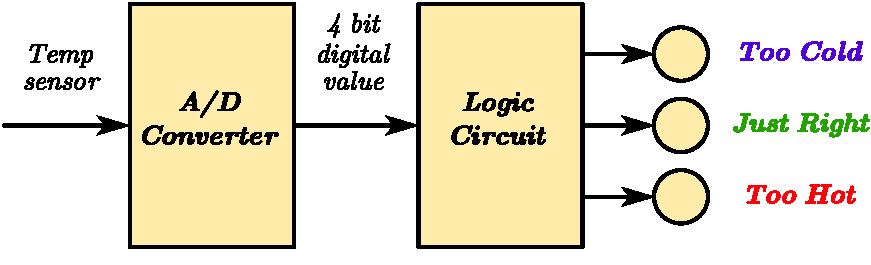
\includegraphics[width=\linewidth]{Graphics/VHDL/Practice 1/Temp_ADC_Logic.pdf}
    \caption{Circuit block representation.}
    \label{fig:tempcircuit}
\end{figure}

As we can see in the diagram, there is a temperature sensor which output is fed into an analog-to-digital converter. The latter outputs a 4 bit digital value which serves as input to the logic circuit that we have to design. This circuit will interpret the  data and, based on it, it will turn on a specific LED to indicate the temperature range that the sensor is measuring, being these states the ones indicated in the diagram\medskip

To aid the design process, a table containing the possible output values of the ADC and their corresponding meaning is given:

\begin{table}[ht]
    \centering
        \begin{tabular}[t]{lcc}
            \toprule
            &\textbf{Digital Values}&\textbf{Category}\\
            \midrule
            &0000-1000&Too cold\\
            &1001-1010&Just right\\
            &1011-1111&Too hot\\
            \bottomrule
        \end{tabular}
        \caption{Possible states.}
\end{table}

Our job will consist in programming the logic circuit in order to obtain the desired behaviour. In this practice, as well as in the rest of the subject, we will make use of the GAL22V10. This IC, commonly found in the DIP package, though old, is still a very good choice for beginners, due to its simplicity and ease of use.\medskip

\newpage

To program the circuit, we will use the proprietary software designed for it, IspLever Classic. This program will allow us to synthesize and implement our VHDL code into the GAL SPLD. The main advantage of PLDs and FPGAs is the ability to program, using code, the HARDWARE part of our circuit, allowing us to obtain higher switching speeds and a faster response compared to what we would obtain if we were to use a microcontroller.\medskip

Writing some pseudocode before programming our circuit will surely come in handy later, as it is a nice way of organising the code and its different parts.

For this simple case, we came up with the following:\medskip

\begin{algorithm}
        \begin{algorithmic}
            \IF{digital value $\leq 8$}
            \STATE light only the \textcolor{blue}{Too Cold} indicator.
            \ELSIF{8 < digital value < 11}
            \STATE light only the \textcolor{green}{Just Right} indicator.
            \ELSE{}
            \STATE light only the \textcolor{red}{Too Hot} indicator.
            \ENDIF
        \end{algorithmic}
\end{algorithm}

Before starting programming our circuit, we will first define the basic parts of any VHDL program:

\subsection{Introduction}

\subsubsection{Library}

One of the most important parts of any VHDL program is the inclusion of several, important libraries.\textbf{Libraries} are pre-written chunks of code that allow us to focus on the development of our code without having to worry too much about the technical and laborious parts of the language itself.

The structure of this part is as follows:

\inputcode{CODES/VHDL/Practice_1/Library.vhd}


Here we can find a library clause, for instance, \textbf{library ieee;} , and a use clause, \textbf{use ieee.std\textunderscore logic\textunderscore 1164.all;}, among others. This gives the code access to all the names declared within package \textbf{std\textunderscore logic\textunderscore 1164} in the library \textbf{ieee}, and to data type \textbf{std\textunderscore logic} in particular.\medskip

We can include other libraries such as \textbf{ieee.std\textunderscore logic\textunderscore arith} which defines some types and basic arithmetic operations for representing integers in standard ways.

\clearpage

\subsubsection{Entity}

An \textbf{entity} can be though of as a black box with inputs and outputs. The entity declaration includes the \textbf{name} of the entity, and a set of port declarations. A \textbf{port} may correspond to a pin on an IC, an edge connector on a board, or any logical channel of communication with a block of hardware.\medskip

Each port declaration includes the \textbf{name of one or more ports}, the \textbf{direction} that information is allowed to flow through the ports \textbf{(in, out or inout)}, and the data type of the ports (i.e., \textbf{std\textunderscore logic}). \medskip

The structure of this part is as follows:

\inputcode{CODES/VHDL/Practice_1/Entity.vhd}


\subsubsection{Architecture}

The \textbf{architecture} is no longer a definition of parameters but the code itself. The architecture describes the design and is bounded to the entity. 

The syntax for VHDL architecture is as follows: 

\inputcode{CODES/VHDL/Practice_1/Architecture.vhd}

In VHDL, it is possible to find more than one architecture. Depending on the complexity of the actions that need to be performed by the PLD/FPGA, we may use concurrent statements, sequential ones -with \textbf{processes}-, or both.\medskip

The architecture has two parts. The declaration part, between the keywords \textbf{\textit{architecture}} and \textbf{\textit{begin}}, in which the interconnection signals, other components referenced by this architecture, or constants are defined and a second part, which starts after the keyword \textbf{\textit{begin}} that includes the statements and assignments and structure of the design.

\clearpage

\subsection{Exercise 1: Temperature Controlled LED Indicator}

Now that every part of the code has been tacked, we will write the actual code that we will program into the GAL:

\inputcode{CODES/VHDL/Practice_1/Temperature.vhd}

\newpage

In order to fully understand the code, we will break it down into small chunks.

\inputcode{CODES/VHDL/Practice_1/Temperature_entity.vhd}

As indicated in Figure \ref{fig:tempcircuit}, we will make use of 4 inputs, tied together in a vector, and 3 outputs, which will be connected to our LEDs. This concludes the entity part of our code.

Now, we will analyse its architecture:

\inputcode{CODES/VHDL/Practice_1/Temperature_entity.vhd}

As we can see, this architecture is sequential, i.e. the statements don't occur at the same time but one after the other. This is illustrated in line 3, in which the keyword \textbf{process} and a sensitivity list containing the vector \textbf{temp} are introduced. Every time that the value of \textbf{temp} changes, the code linked to that process is run. In our case, this code checks the value of the temperature and turns one of the three LEDs on based on the reading.

\newpage

After programming the code, it is time to compile it using \textbf{IspLeverClassic}. To do this, we will click on \textbf{Create Fuse Map} and wait for it to finish. Once compiled, we will flash the JEDEC file, which contains the fuse arrangement, into the GAL. The set up process won't be included into the reports as it is quite long and not really worth the explanation.\medskip

\begin{figure}[H]
    \centering
    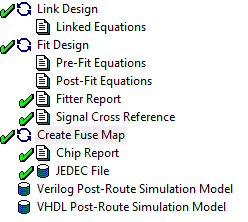
\includegraphics[scale = 0.85]{Graphics/VHDL/Practice 1/ISPLever.PNG}
    \caption{ISPLever.}
    \label{fig:ISPLever}
\end{figure}

Due to the simplicity of the GAL, the pin assignments are automatically performed by the software, so we have to check which pins the compiler decided to use. To do this, we will make use of the \textbf{Chip Report} pop-up menu.

\begin{figure}[H]
    \centering
    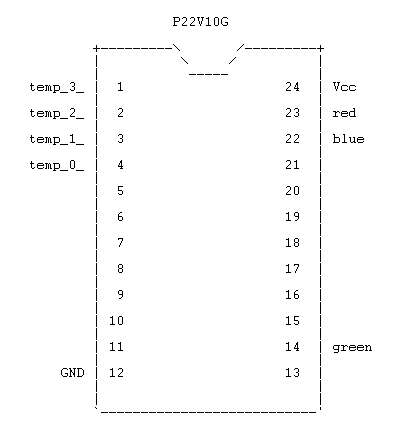
\includegraphics[scale=0.7]{Graphics/VHDL/Practice 1/Chip_Report.PNG}
    \caption{Chip Report Output.}
    \label{fig:CHIP_REPORT}
\end{figure}

\newpage

Once everything checks, we will move on to simulating the circuit before finally assembling it. To do this, we will make use of ISIS Proteus, a well-know electronics simulation software.\medskip

Knowing the pin assignments makes the task of simulating the circuit very simple, as the only thing required is to follow the \textbf{Chip Report's} connections in Proteus.

\begin{figure}[H]
    \centering
    
    \ifnum\value{ANIMATION}=1 {
        \animategraphics[controls,loop,scale=1.2]{2}{Graphics/VHDL/Practice 1/ANIMATION/F}{0}{15}
    } 
    \else {
        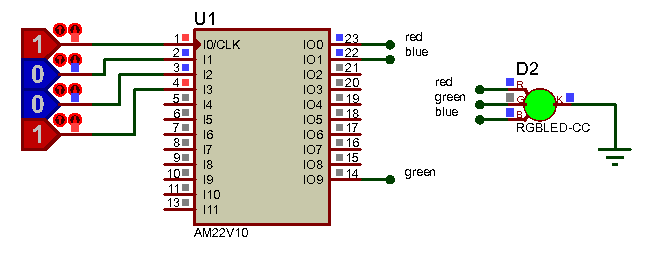
\includegraphics[scale=1.2]{Graphics/VHDL/Practice 1/ANIMATION/F9.PDF}
    }\fi
    
    \caption{Proteus assembly.}
    \label{fig:PROTEUS_TEMP}
\end{figure}

Now that we have checked that the circuit works as intended, we can proceed to the real assembly. Again, this is just a matter of following the previous connections but this time using a protoboard and some hook-up wires. \medskip

As expected, everything worked great.

\newpage
\section{Laboratory Lecture 2: Flip Flops}
\label{sec:FLIP_FLOPS}

The main objective of this lab lecture is to learn about the operation of Flip Flops. In particular, we will discuss how JK flip flops work as well as some of their applications.

\subsection{Introduction}

A flip flop, also known as latch or bistable multivibrator, is a type of circuit that has two states, one of them represents a \textit{one} and the other one a \textit{zero}, i.e. a single bit of data. They are commonly used to store information in digital circuits.\medskip 

Flip flops can be edge-triggered, that is synchronous/clocked, or level triggered, that is asynchronous. In order to control them, we have to apply specific signals to the inputs, following their truth table.\medskip

Some examples of flip flops may include D Flip flops, D Latch Flip flops, SR Flip flops, and JK Flip flops, to name a few. In this practice we are going to work with the latter.

\subsubsection{JK Flip Flops}

Before diving into what a JK Flip Flop is, we will briefly talk about SR Flip Flops, as they are the old and troublesome early version of a JK one.\medskip

SR Flip Flops, also known as SR Latch, are one the most basic sequential logic circuits. They act as a one-bit memory, so a bistable device, that possesses 2 inputs. On the one hand, \textit{SET}, which will output a 1 and is usually labelled \textit{S}, and \textit{RESET}, which will output a 0, and is usually labelled \textit{R}. \medskip

Note than we can also find a clocked, or synchronous variation of the SR Flip Flop. The latter will have an extra input, \textit{CLK} and it will only trigger on the positive edge transitions of the clock.\medskip

Obviously, \textit{SR} stands for "Set-Reset". As we have previously said, the reset input resets the flip flop, that is, it makes the output, Q, go back to its original state of 0. The different input configurations will define the behaviour of the output following this fashion:\medskip


\begin{minipage}{\textwidth}
    \begin{minipage}[b]{0.49\textwidth}
        \centering
        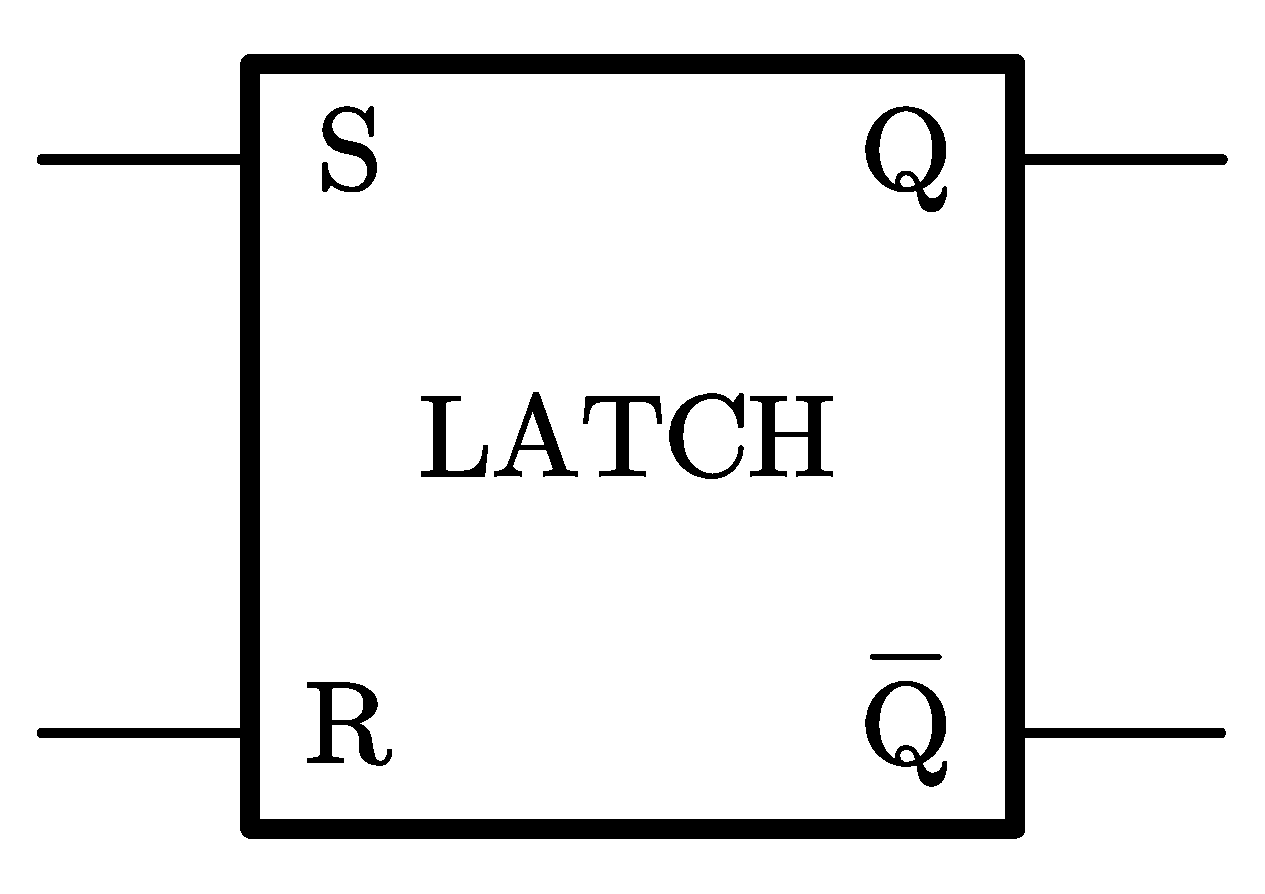
\includegraphics[scale=0.2]{Graphics/VHDL/Practice 2/GRAPHICS/LOGIC GATES/SR ASYNCH.pdf}
        \captionof{figure}{SR Asynchronous Flip Flop.}
        \label{fig:SR_Asynch}
    \end{minipage}
    \hfill
    \begin{minipage}[b]{0.49\textwidth}
        \centering
             \begin{tabular}[t]{lccc}
                \toprule
                &\textbf{SET}&\textbf{RST}&\textbf{Q}\\
                \midrule
                & 0 & 0 & $Q_0 \text{ No change}$\\
                & 1 & 0 & Q = 1\\
                & 0 & 1 & Q = 0\\
                & 1 & 1 & Invalid\\
                \bottomrule
            \end{tabular}
        \captionof{table}{SR Flip Flop's Truth Table.}
    \end{minipage}
\end{minipage}\textbf{}

\clearpage

As we can deduce from the table, this type of flip flops pose a problem when both the \textit{S} and the \textit{R} inputs are 1, since the output state is invalid and cannot be predicted.\medskip

To solve this problem, we will make use of a \textbf{JK Flip Flop}. JK Flip flops, in a nutshell, solve this problem by having the output toggle when both inputs \textit{J} and \textit{K}, which correspond to the \textit{S} and \textit{R} terminals respectively, are 1. The truth table of this type of flip flop is as follows:\bigskip

\begin{minipage}{\textwidth}
    \begin{minipage}[b]{0.49\textwidth}
        \centering
        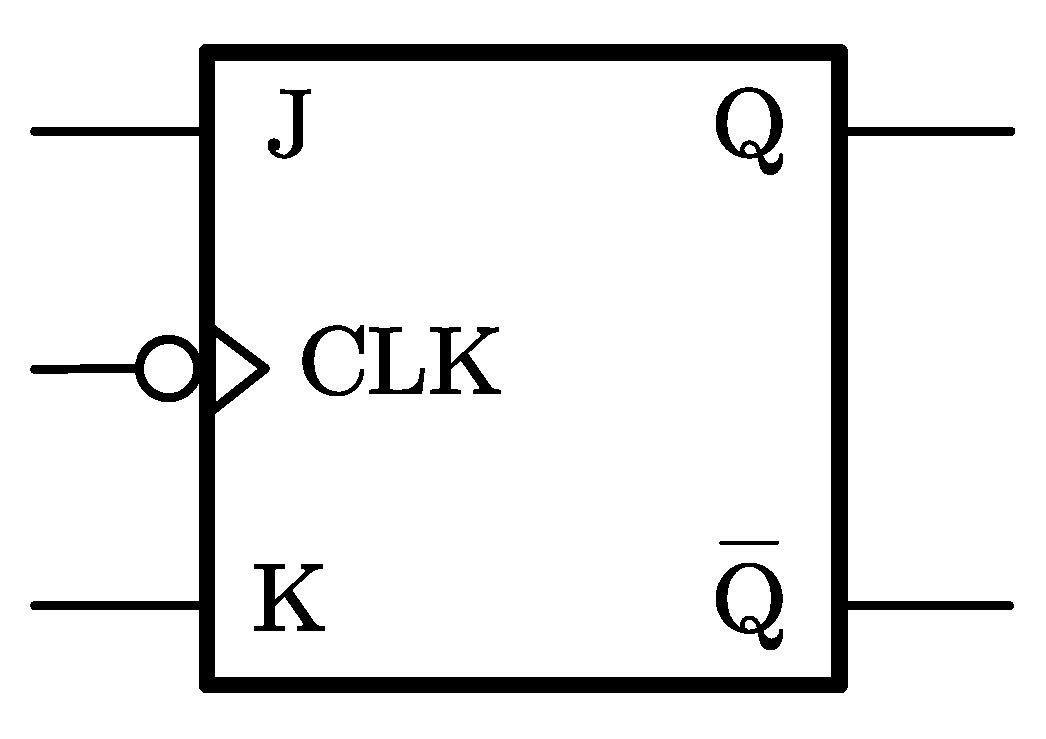
\includegraphics[scale=0.25]{Graphics/VHDL/Practice 2/GRAPHICS/LOGIC GATES/JK SYNCH.pdf}
        \captionof{figure}{JK Synch. Flip Flop.}
        \label{fig:JK_Synch}
    \end{minipage}
    \hfill
    \begin{minipage}[b]{0.49\textwidth}
        \centering
            \begin{tabular}[t]{lcccc}
                \toprule
                &\textbf{J}&\textbf{K}&\textbf{CLK}&\textbf{Q}\\
                \midrule
                &0&0& $\uparrow$ & $Q_0 \text{ No change}$\\
                &1&0& $\uparrow$ & Q = 1\\
                &0&1& $\uparrow$ & Q = 0\\
                &1&1& $\uparrow$ & $\overline{Q_0} \text{ Toggles}$\\
                \bottomrule
            \end{tabular}
        \captionof{table}{JK's Synch. Truth Table.}
        \label{table:JK_Synch_TT}
    \end{minipage}
\end{minipage}

\vspace{0.5cm}

It is possible to find an asynchronous version of the JK Flip Flop as well. This version has two extra pins, \textit{PRESET} and \textit{CLEAR}, which, if active, will turn the output $Q$ to 0, if the \textit{PRESET} is connected to 1 and the \textit{CLEAR} to 0. Alternatively, they will turn the output $Q$ to 1 if the \textit{PRESET} is connected to 0, and the \textit{CLEAR} to 1. We can visualise this in the following truth table: 

\vspace{0.7cm}

\begin{minipage}{\textwidth}
    \begin{minipage}[b]{0.49\textwidth}
        \centering
        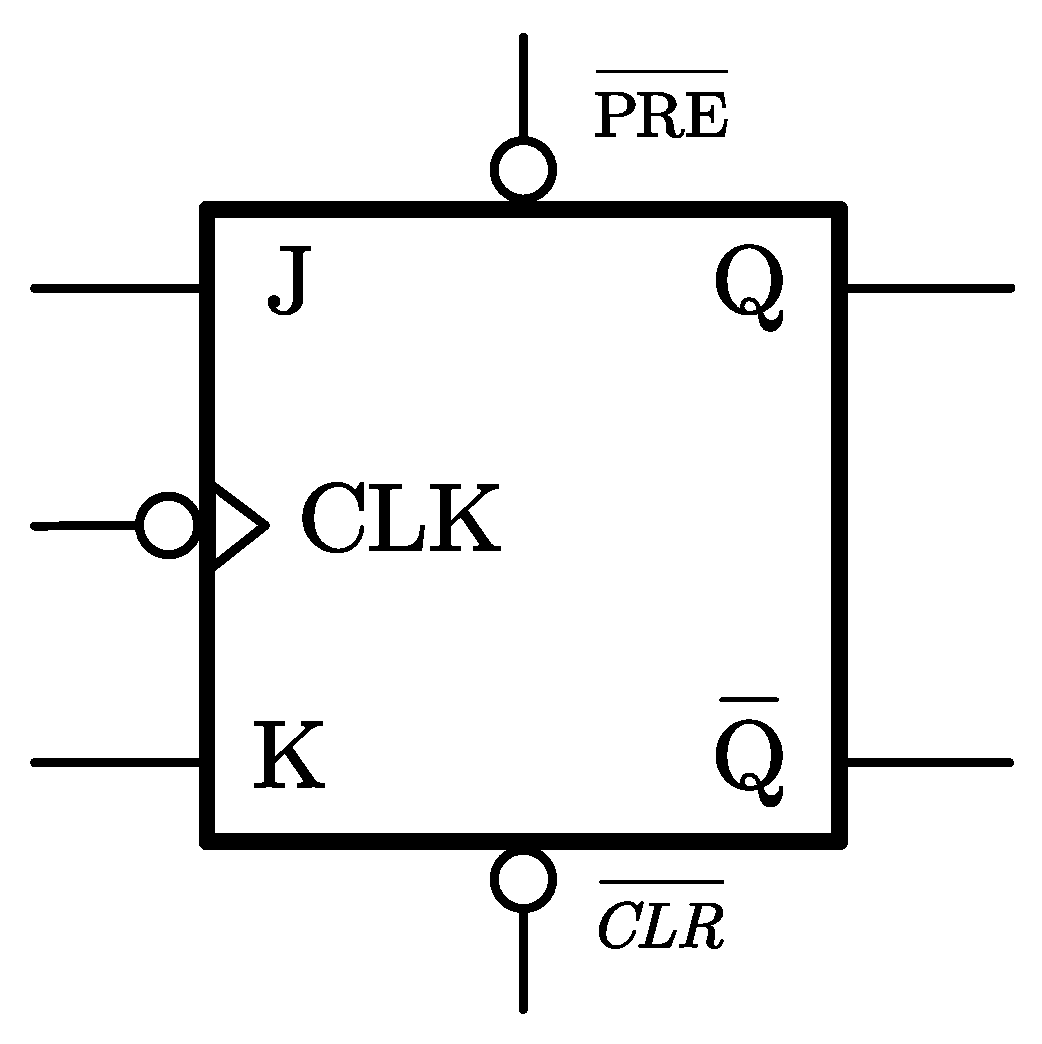
\includegraphics[scale=0.25]{Graphics/VHDL/Practice 2/GRAPHICS/LOGIC GATES/JK ASYNCH.pdf}
        \captionof{figure}{JK Asynch. Flip Flop.}
        \label{fig:JK_Asynch}
    \end{minipage}
    \hfill
    \begin{minipage}[b]{0.49\textwidth}
        \centering
            \begin{tabular}[t]{lcccccc}
                \toprule
                & \textbf{J} & \textbf{K} & \textbf{CLK} & $\overline{\mathbf{PRE}}$ & $\overline{\mathbf{CLR}}$ & \textbf{Q}\\
                \midrule
                & 0 & 0 & $\downarrow$ & 1 & 1 & $Q_0$\\
                & 1 & 0 & $\downarrow$ & 1 & 1 & 1\\
                & 0 & 1 & $\downarrow$ & 1 & 1 & 0\\
                & 1 & 1 & $\downarrow$ & 1 & 1 & $\overline{Q_0}$\\
                \midrule
                & X & X & X & 0 & 0 & Inv\\
                & X & X & X & 0 & 1 & 1\\
                & X & X & X & 1 & 0 & 0\\
                \bottomrule
            \end{tabular}
        \captionof{table}{JK's Asynch. Truth Table.}
        \label{table:JK_Asynch_TT}
    \end{minipage}
\end{minipage}\textbf{}

\newpage

Now that we have established the basics, we will move on to completing the laboratory session.

\subsection{Exercise 1: JK Flip Flop}

\subsubsection{Asynchronous \textit{PRE} and \textit{CLR} effect on Q}

In order to complete this part, we will make use of the program Proteus, as per usual. We will simply follow Table \ref{table:JK_Asynch_TT} in order to check the output when \textit{PRE} and \textit{CLR} change.

\begin{figure}[H]
    \centering
    
    \ifnum\value{ANIMATION}=1 {
        \animategraphics[controls,loop,scale=1.4]{1}{Graphics/VHDL/Practice 2/GRAPHICS/ANIMATION/JK ASYNCH/F}{0}{2}
    } 
    \else {
        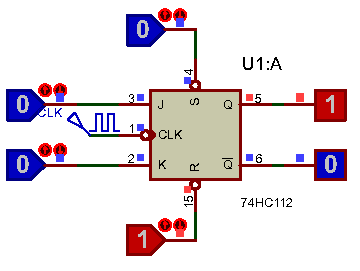
\includegraphics[scale=1.4]{Graphics/VHDL/Practice 2/GRAPHICS/ANIMATION/JK ASYNCH/F1.PDF}
    }\fi
    
    \caption{Proteus assembly.}
    \label{fig:PROTEUS_JK_ASYNCH}
\end{figure}

In the simulation, we can not only see that the output, $Q$, is correct, but that it also does not depend on the values of \textit{J}, \textit{K}, and \textit{CLK}. 

\subsubsection{Synchronous \textit{J} and \textit{K} effect on Q}

For this part, as we are working with a Synchronous circuit, both \textit{PRE} and \textit{CLR} have to be tied to their inactive state, in this case, since they are active low, we will tie them to 1.

Again, we have to check that the circuit behaves as expected, that it, that it follows Table \ref{table:JK_Synch_TT}

\newpage

To achieve this, we will use Proteus once more.

\begin{figure}[H]
    \centering
    
    \ifnum\value{ANIMATION}=1 {
        \animategraphics[controls,loop,scale=1.4]{1}{Graphics/VHDL/Practice 2/GRAPHICS/ANIMATION/JK SYNCH/F}{0}{5}
    } 
    \else {
        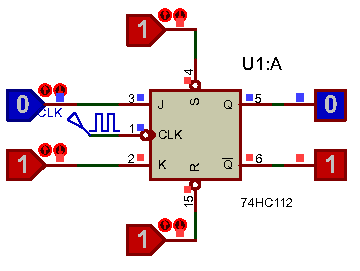
\includegraphics[scale=1.4]{Graphics/VHDL/Practice 2/GRAPHICS/ANIMATION/JK SYNCH/F2.PDF}
    }\fi
    
    \caption{Proteus assembly.}
    \label{fig:PROTEUS_JK_SYNCH}
\end{figure}

As we can see, the circuit behaves as expected.


\subsection{Exercise 2: T Flip Flop from JK Flip Flop}

In this exercise we are asked to create a T Flip Flop using a JK one. To do this we have to take Table \ref{table:JK_Synch_TT} into account, as it clearly states that when both inputs, \textit{J} and \textit{K} are tied to 1, and a falling edge of the clock occurs -in the case of a 74HC112-, the output toggles, which is precisely what we aim to obtain.


\begin{figure}[H]
    \centering
    
    \ifnum\value{ANIMATION}=1 {
        \animategraphics[controls,loop,scale=1.4]{2}{Graphics/VHDL/Practice 2/GRAPHICS/ANIMATION/T/F}{0}{1}
    } 
    \else {
        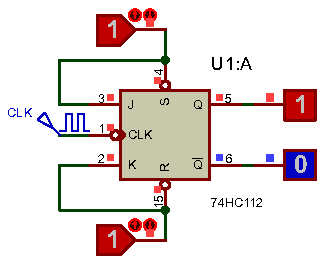
\includegraphics[scale=1.4]{Graphics/VHDL/Practice 2/GRAPHICS/ANIMATION/T/F1.PDF}
    }\fi
    
    \caption{Proteus assembly.}
    \label{fig:PROTEUS_T}
\end{figure}

\clearpage

One of the most important applications of this type of gate is to build a frequency divider. Since we are using a 74HC112 as a T Flip Flop, if we apply a \textit{CLK} signal with a duty cycle of $50\%$ to the clock input, the output $Q$ will toggle every time a falling edge occurs, that is, every full cycle, effectively dividing the input frequency by 2. We can visualise this in the following timing diagram: \medskip

\begin{figure}[H]
    \centering
    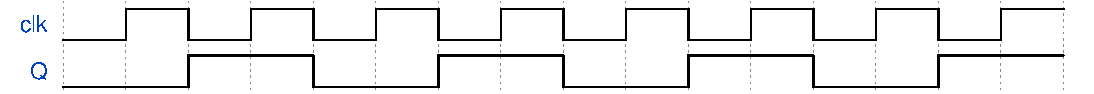
\includegraphics[scale = 0.73]{Graphics/VHDL/Practice 2/GRAPHICS/TIMING/EX2.pdf}
    \caption{Timing diagram of a 2-bit frequency divider.}
    \label{fig:timing_1}
\end{figure}

\subsection{Exercise 3: T Flip Flop Asynchronous counter}

Now that we have established how to build a frequency divider, we will focus on its applications. In particular, we will build a binary counter, which will be fed to a BCD to 7 segment display decoder, so as to help us visualise the output.\medskip

In Figure \ref{fig:timing_1}, we can already see the the behaviour that we are aiming for. In the first division, the \textit{Q} and the \textit{clk} signals have a logic level of 0, or 00 in binary. This value turns into a 01 in the second division, 10, in the third, and finally 11 in the fourth. Translating these numbers into decimal yields 0, 1, 2, 3, so we can say that Figure \ref{fig:timing_1} represents a 2 bit binary counter.\medskip

In order to be able to display numbers up to 7, we will need a 3 bit binary counter. Building it is just a matter of concatenating 2 T Flips Flops following this fashion:

\begin{figure}[H]
    \centering
    
    \ifnum\value{ANIMATION}=1 {
        \animategraphics[controls,loop,scale=0.85]{2}{Graphics/VHDL/Practice 2/GRAPHICS/ANIMATION/7_SEG/F}{0}{7}
    } 
    \else {
        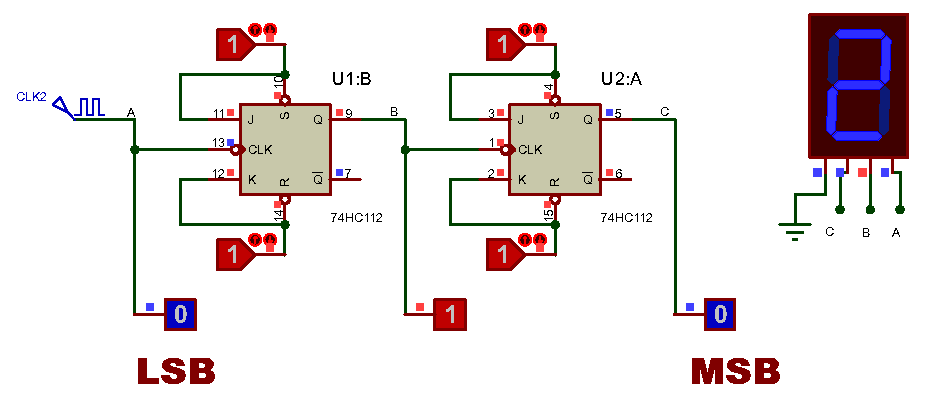
\includegraphics[scale=0.85]{Graphics/VHDL/Practice 2/GRAPHICS/ANIMATION/7_SEG/F2.PDF}
    }\fi
    
    \caption{Proteus assembly.}
    \label{fig:PROTEUS_7_SEG}
\end{figure}

\clearpage

If we look at the output signals with a logic analyser, we will see the following:\medskip

\begin{figure}[H]
    \centering
    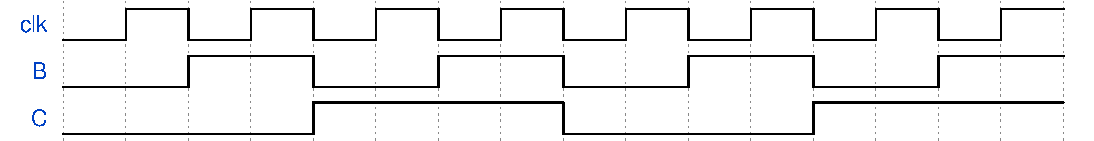
\includegraphics[scale = 0.73]{Graphics/VHDL/Practice 2/GRAPHICS/TIMING/EX3.pdf}
    \caption{Timing diagram of a 3-bit frequency divider.}
    \label{fig:timing_2}
\end{figure}

The only problem that this configuration poses, is that a small glitch is produced at the output due to the propagation time of the \textit{CLK} signals, as the output of the first T Flip Flop is fed into the input of the next one and so on.\medskip 

One possible solution would be to add a capacitor connected to ground to each of the 3 outputs, in order to smooth out the peak and make the transition more visually appealing and less prone to error.

\clearpage

\section{Laboratory Lecture 2 BIS: 555 Timer}

\subsection{Introduction}

Up until this point we have seen how to manipulate clock signals by using frequency dividers, but what if we want to obtain a specific type of output response, for instance a single pulse or a clock with a duty cycle different from 50\% ? In this case, a multivibrator circuit is needed. \medskip

These type of integrated circuits use an RC timer to set the pulse duration and, depending on the manufacturer, they may work in different modes, i.e.:

\begin{enumerate}
    \item Clock generator circuits (Astable Multivibrator)
    
    \item One-Shot (Monostable Multivibrator)
    \begin{itemize}
        \item Retriggerable
        \item Non-Retriggerable
    \end{itemize}
\end{enumerate}

\subsubsection{Astable Multivibrator}

The first type of circuit, the \textbf{Astable Multivibrator}, is what is commonly referred to as \textbf{"Clock"}. These simple circuits basically switch back and forth between two unstable states with a specific duty cycle\footnote{The duty cycle of a digital circuit is the percentage of the ratio of pulse duration, or pulse width to the total period. It can be expressed as: 

\begin{equation*}
    D = \frac{t_{ON}}{t_{ON} + t_{OFF}} \cdot 100
    \label{fig:DUTY}
\end{equation*}
} set by an RC circuit. \medskip

In the previous section we have seen how modify a clock signal to obtain a specific output frequency, taking into account the limitations of an even division of course. The problem with this type of circuits is that they cannot provide custom duty cycles, which are needed in real case scenarios. That is when astable circuits come in handy.\medskip

\subsubsection{Monostable Multivibrator}

On the other hand, we can also find \textbf{Monostable Multivibrators}, commonly referred to as \textbf{"One-Shots"}. These type of circuits, as the name suggests, only output a single pulse when triggered, that is, they have only one stable state. The change from stable to quasi-stable occurs for a fixed time period $\mathbf{t_{p}}$ or $\mathbf{t_{w}}$ which is determined by an RC constant as well.\medskip

These circuits are readily available and they usually come in two forms, i.e. a retriggerable and a non-retriggerable one. When a retriggerable one-shot is triggered before the end of the pulse, the pulse duration $\mathbf{t_{p}}$, is restarted. Contrarily, when a non-retriggerable monostable is triggered before the end of the pulse, the output remains the same, in other words, the input is ignored until the output returns to the steady state.\medskip


\clearpage

We can visualise their behaviour in the following graphs:

\begin{figure}[H]
    \centering
    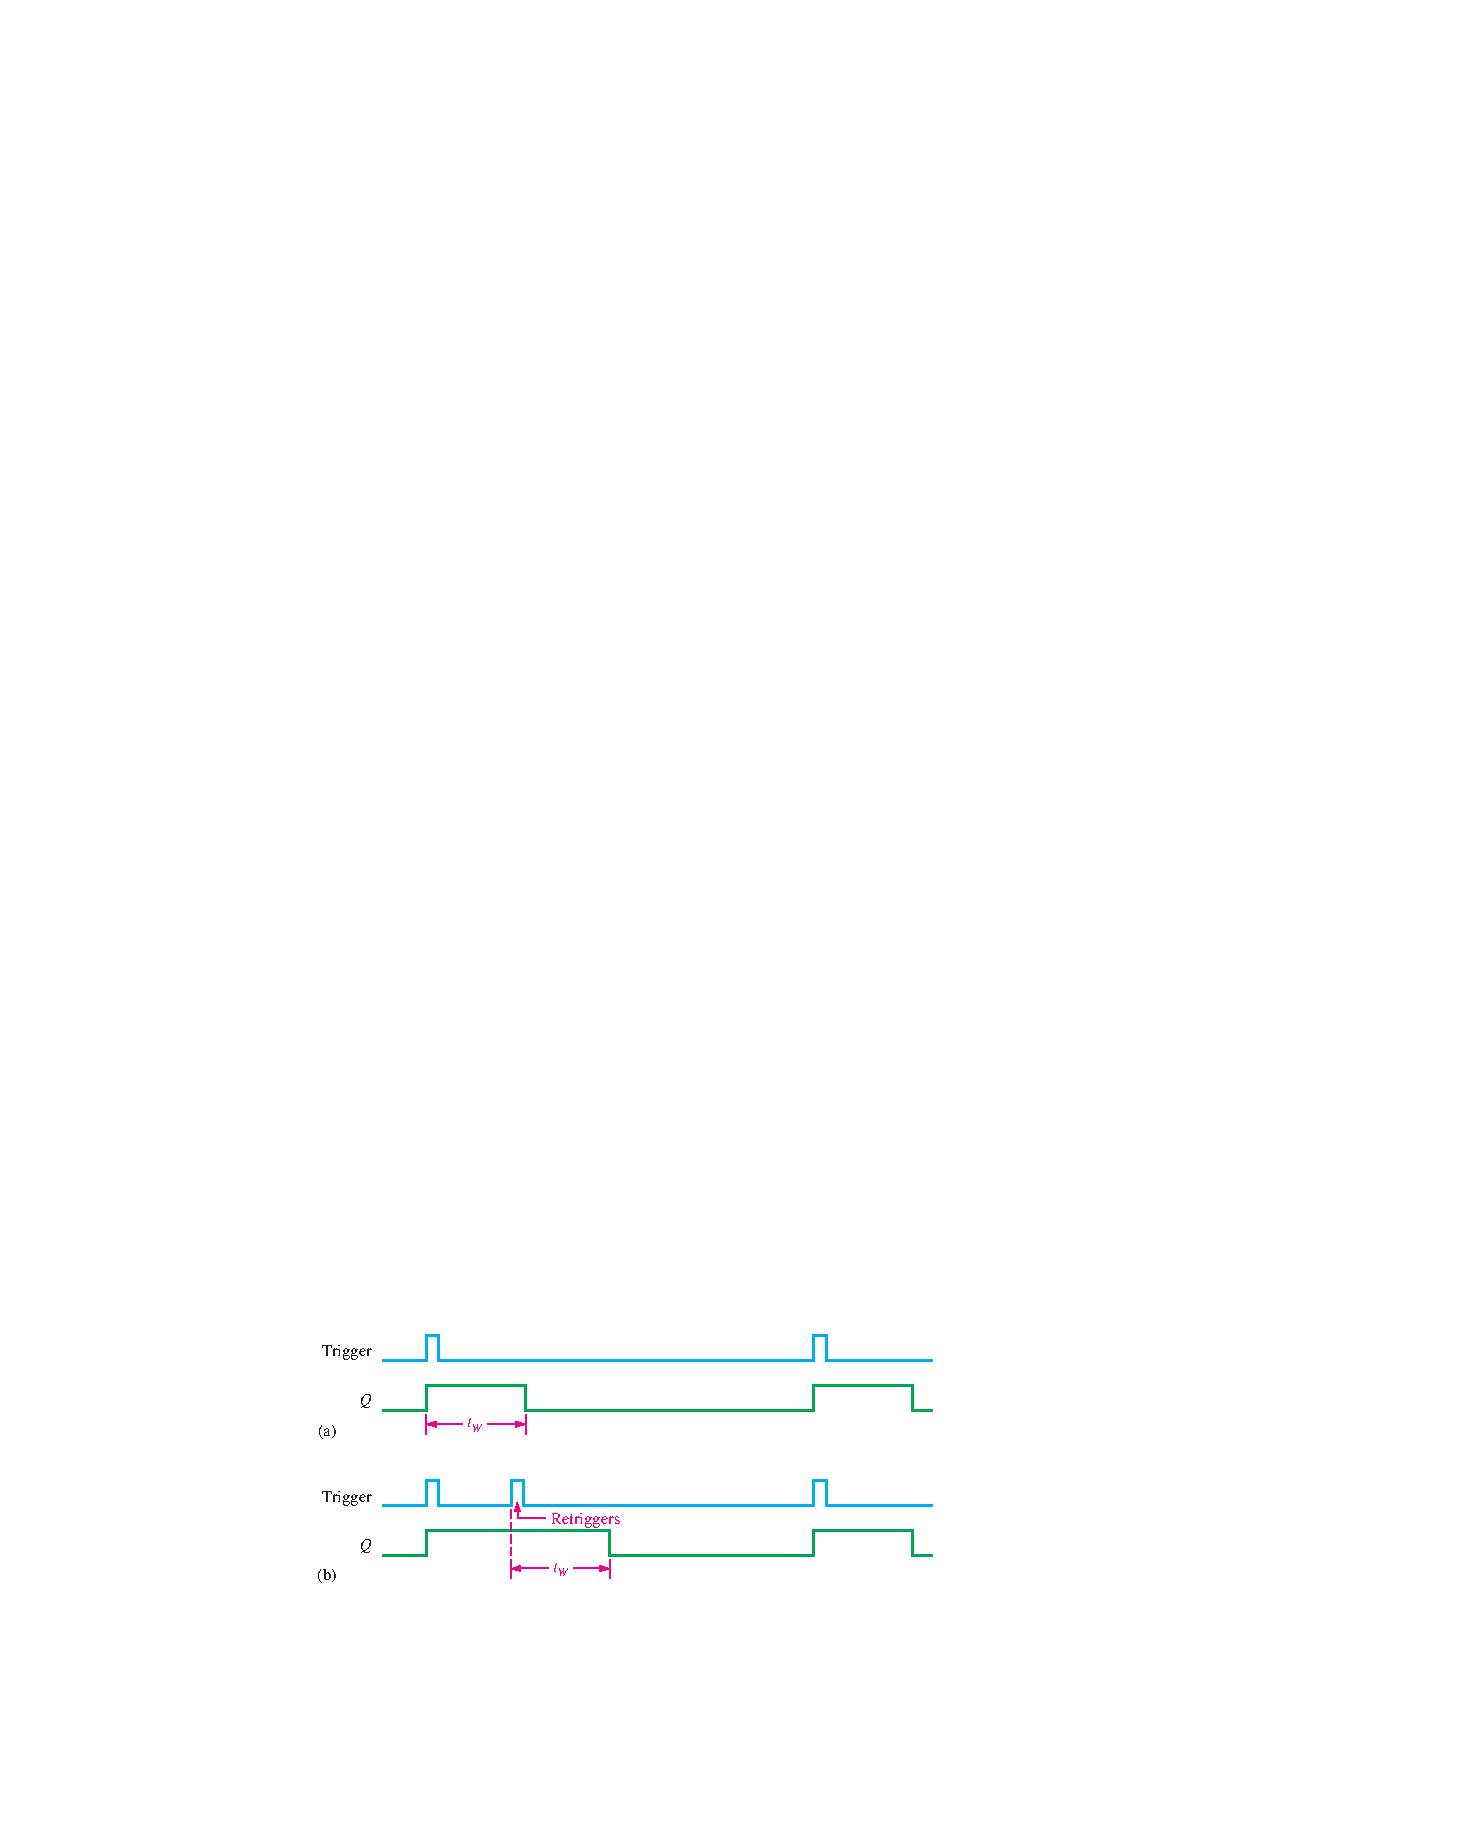
\includegraphics[scale = 1]{Graphics/VHDL/Practice 2/GRAPHICS/MONOSTABLE/RETRIGGERABLE.pdf}
    \caption{Retriggerable Monostable. ~\autocite{FLOYD}}
    \label{fig:RETRIGGERABLE}
\end{figure}

\begin{figure}[H]
    \centering
    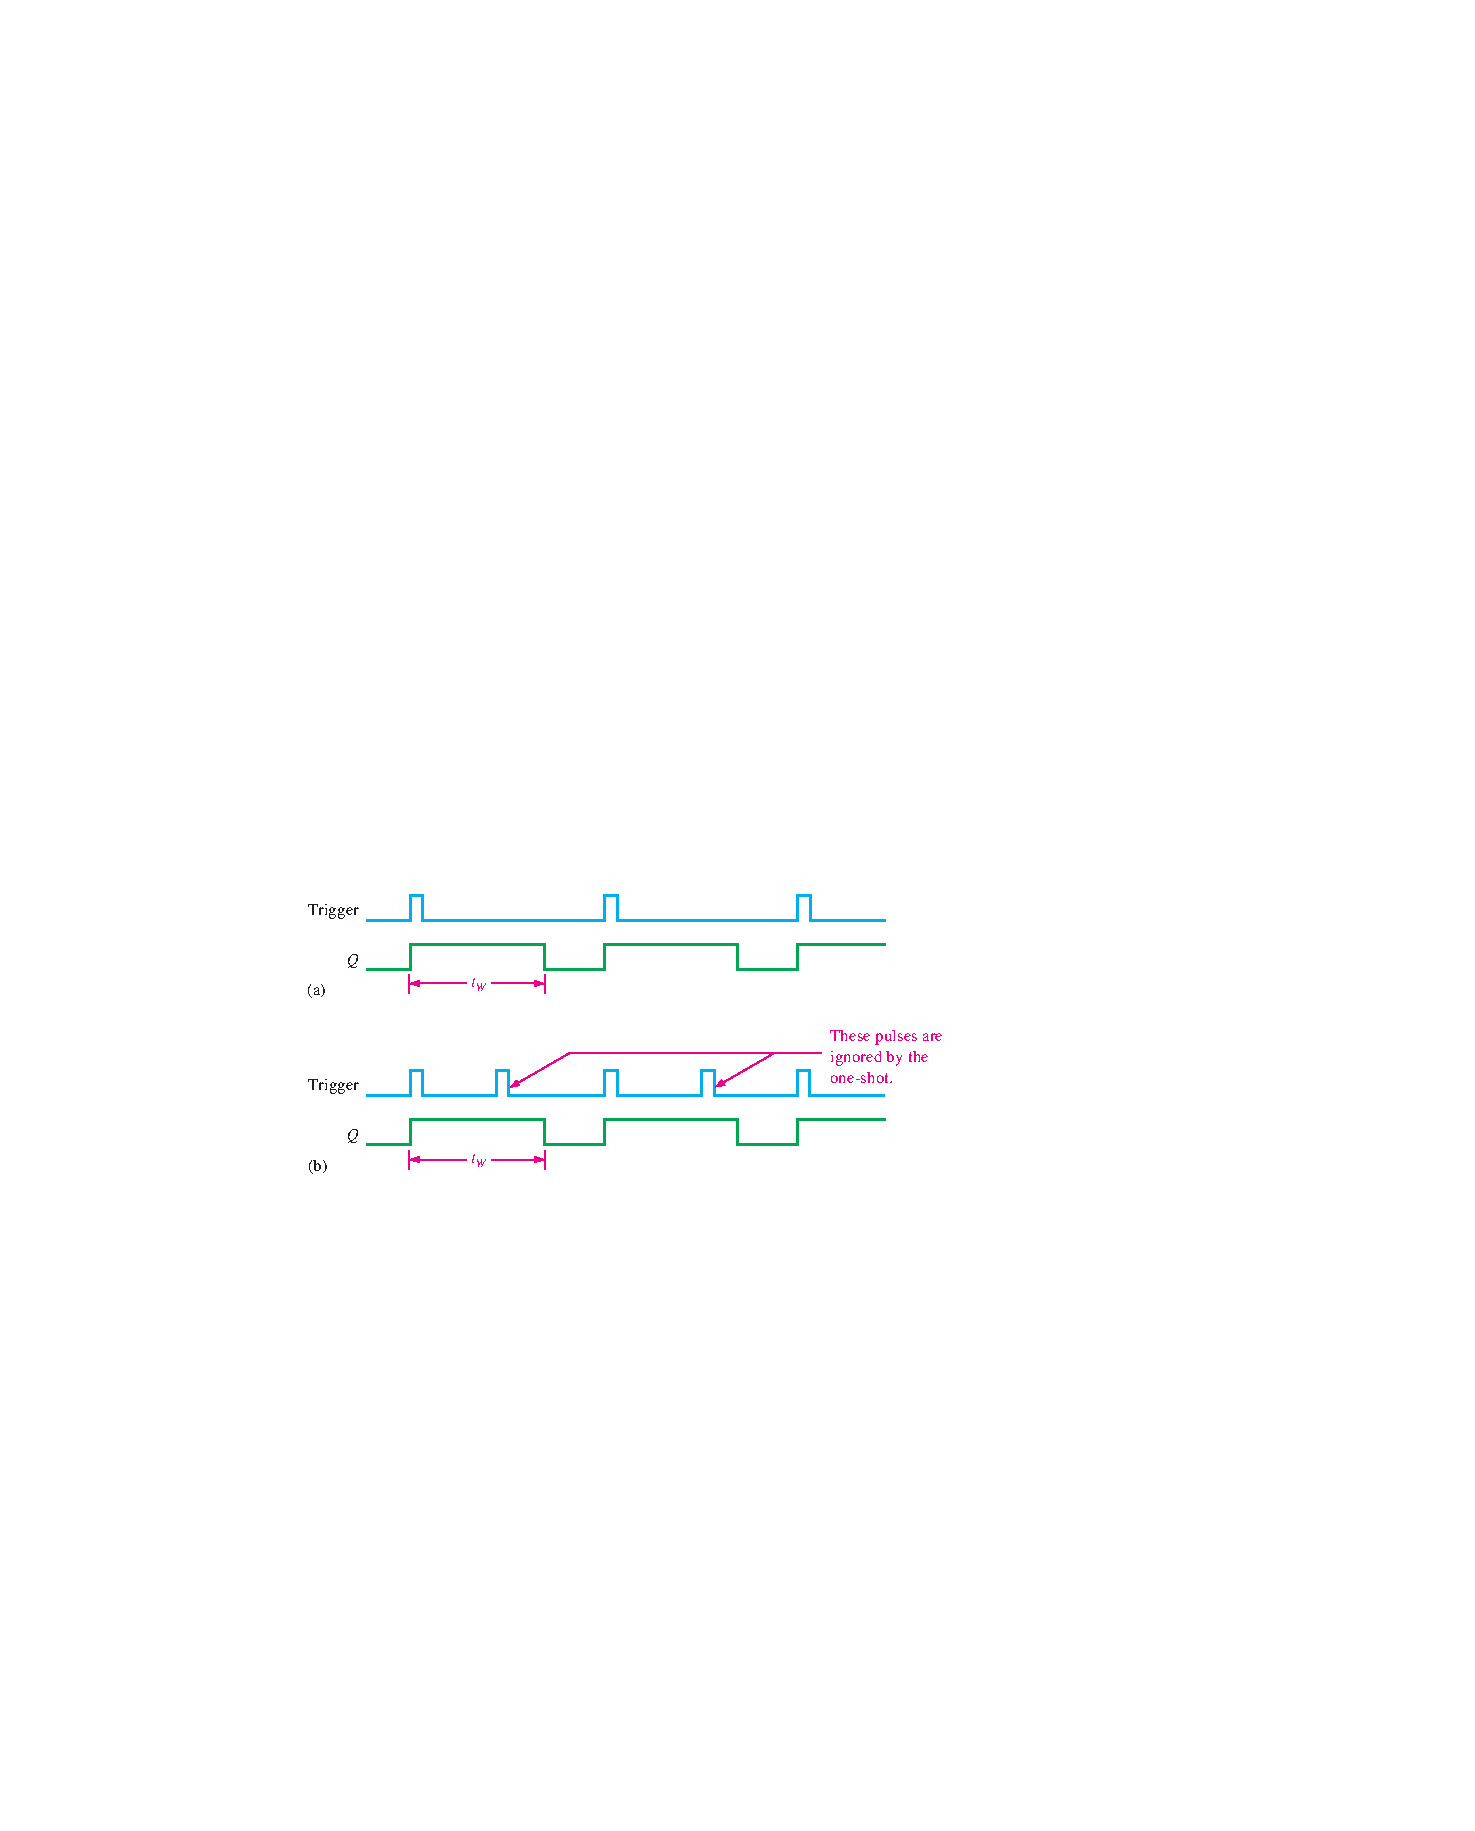
\includegraphics[scale = 1]{Graphics/VHDL/Practice 2/GRAPHICS/MONOSTABLE/NON-RETRIGGERABLE.pdf}
    \caption{Non-Retriggerable Monostable. ~\autocite{FLOYD}}
    \label{fig:NON-RETRIGGERABLE}
\end{figure}


Both monostables, as well as the astable one, can be implemented using VHDL, but we will not dive into this, as it is not required in this practice, though they can be found \href{https://drive.google.com/open?id=1J-T80ZyF3isizOMjBf8xZOD7rw0KesP-}{\textbf{here}}.

\clearpage

\subsection{555 Timer}

Now that every type of multivibrator has been introduced, we will discuss the 555 timer. This timer is a TTL-compatible device that can operate in both of the modes described above. The heart of the 555 timer is composed of two voltage comparators and a SR Latch (See \ref{fig:SR_Asynch}). \medskip

The comparators are devices whose outputs are HIGH when the voltage on the positive (\texttt{+}) input is greater than the voltage on the negative (\texttt{-}) input and LOW when the (\texttt{-}) input voltage is greater than the (\texttt{+}) input voltage. \medskip

The voltage divider consisting of three 5 k$\Omega$ resistors provides a trigger level of $\frac{1}{3}$ VCC and a threshold level of $\frac{2}{3}$ VCC. The control voltage input (pin 5) can be used to externally adjust the trigger and threshold levels to other values if necessary.\medskip 

When the normally HIGH trigger input momentarily goes below $\frac{1}{3}$ VCC, the output of comparator B switches from LOW to HIGH and sets the S-R latch, causing the output (pin 3) to go HIGH and turning the discharge transistor Q1 off.\medskip

The output will stay HIGH until the normally LOW threshold input goes above $\frac{2}{3}$ VCC and
causes the output of comparator A to switch from LOW to HIGH. This resets the latch,
causing the output to go back LOW and turning the discharge transistor on. The external
reset input can be used to reset the latch independent of the threshold circuit. The trigger
and threshold inputs (pins 2 and 6) are controlled by external components connected to
produce either monostable or astable action. ~\autocite{FLOYD}


\begin{figure}[H]
    \centering
    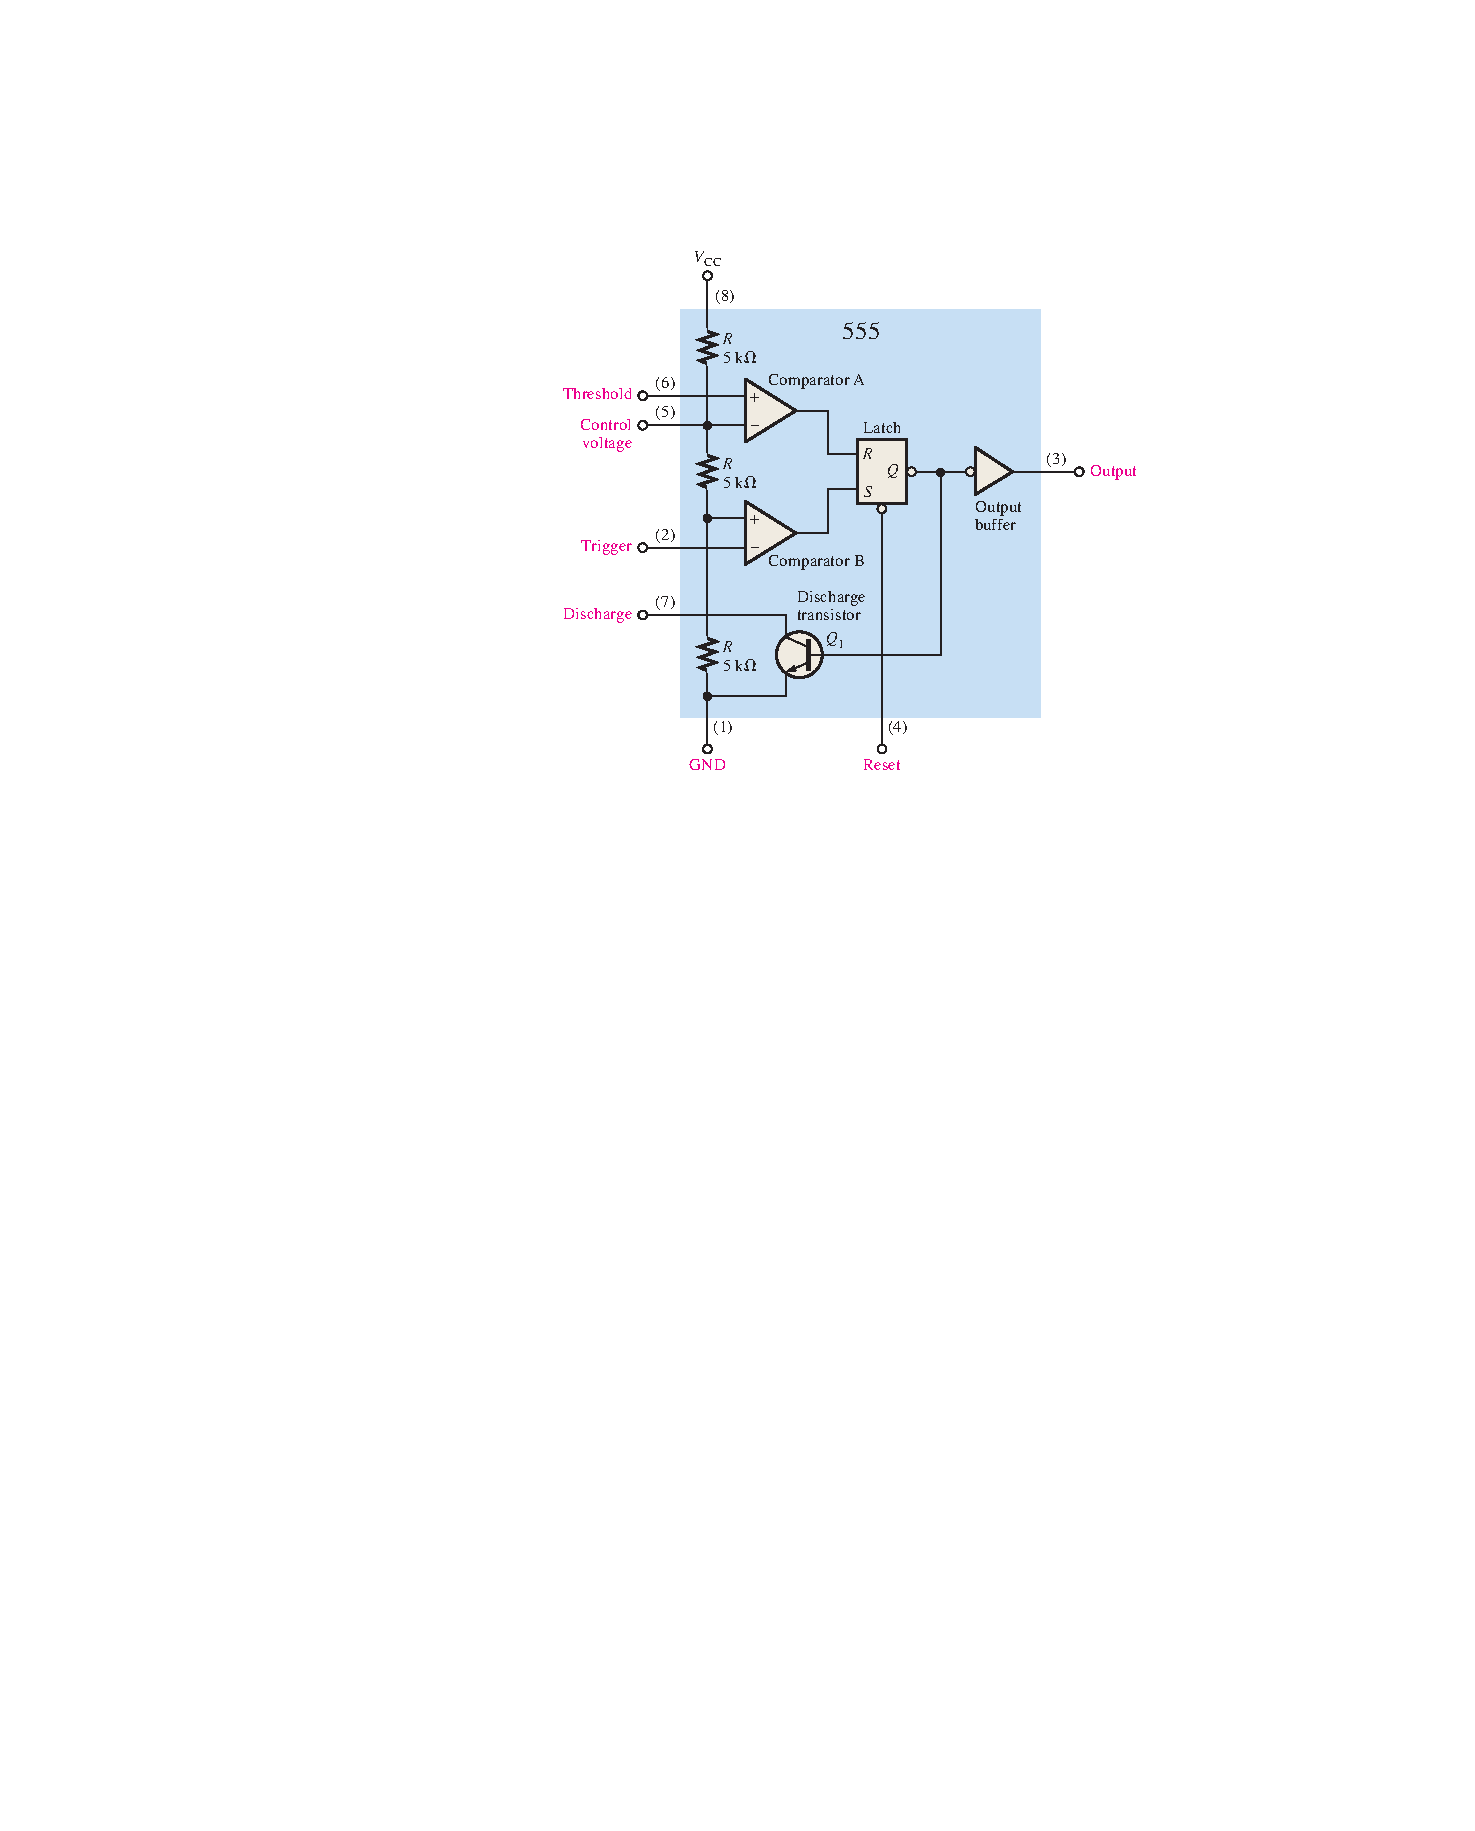
\includegraphics[scale = 0.99]{Graphics/VHDL/Practice 2/GRAPHICS/555/GRAPHS/DATASHEETS/555_INTERNALS.pdf}
    \caption{Internal functional diagram of a 555 timer. ~\autocite{FLOYD}}
    \label{fig:555_DIAGRAM}
\end{figure}


\subsubsection{Astable 555}

As we have mentioned before, the 555 timer can be configured as a basic \textbf{Astable Multivibrator} following the circuit down below:

\begin{figure}[H]
    \centering
    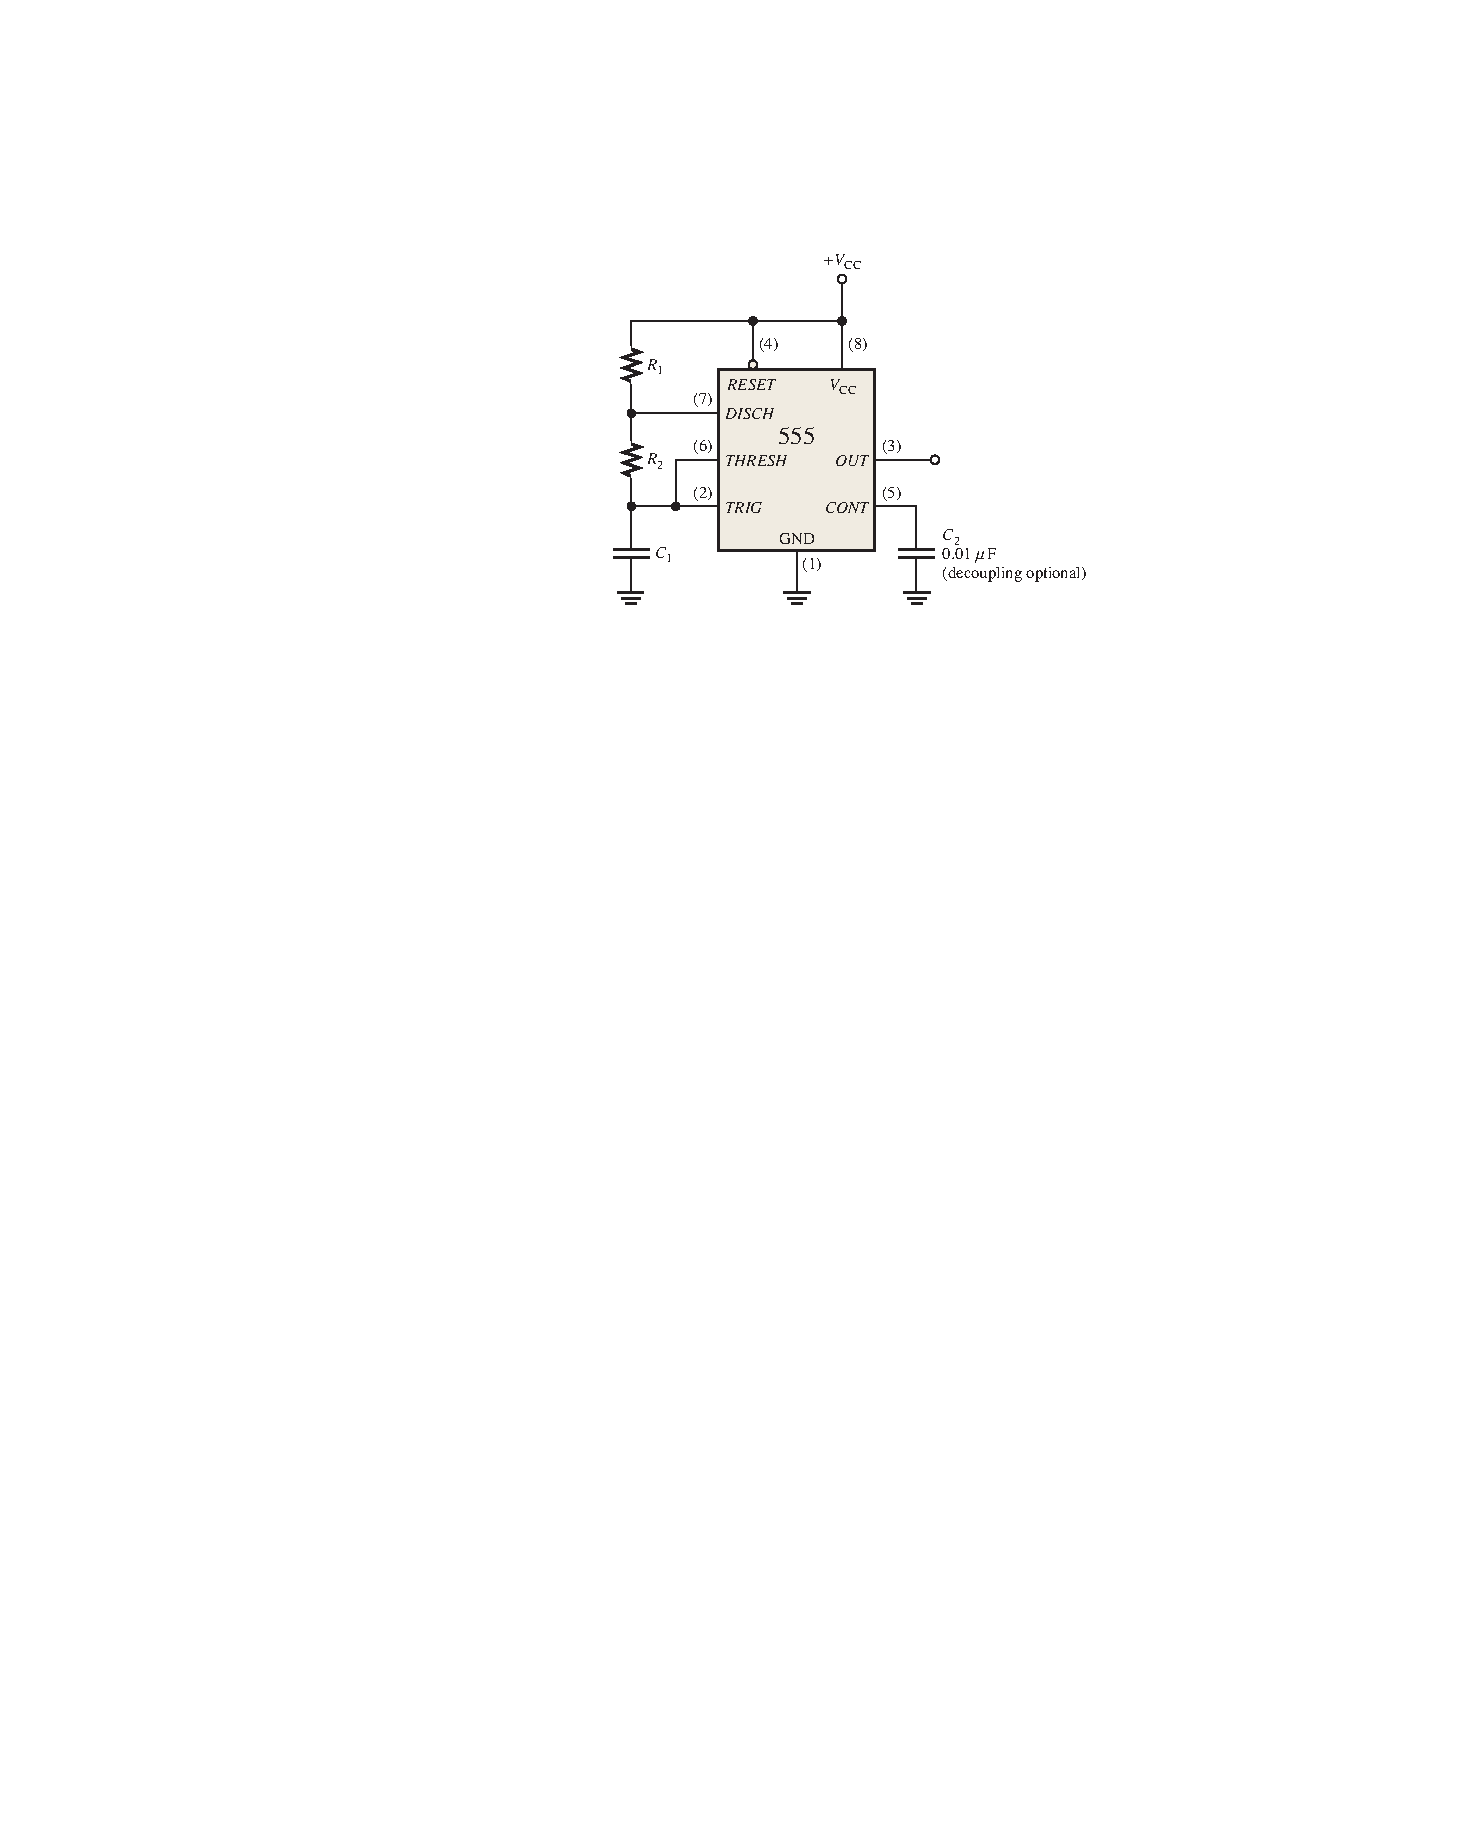
\includegraphics[scale = 1]{Graphics/VHDL/Practice 2/GRAPHICS/555/GRAPHS/MODES/ASTABLE.pdf}
    \caption{555 timer connected as an astable multivibrator (oscillator). ~\autocite{FLOYD}}
    \label{fig:ASTABLE}
\end{figure}

In this circuit C1 charges through R1 and R2 and discharges through only R2. The output frequency is given by:

\begin{equation*}
    f = \frac{1.44}{(R_1 + 2\cdot R_2) \cdot C_1}
\end{equation*}

\vspace{0.25cm}

In order to help us find a set of suitable component values, the manufacturer provides a chart that shows sets of compatible and valid configurations. Besides, some useful equations are provided:

\vspace{0.6cm}

\begin{minipage}{\textwidth}
    \begin{minipage}[c]{0.49\textwidth}
        \centering
        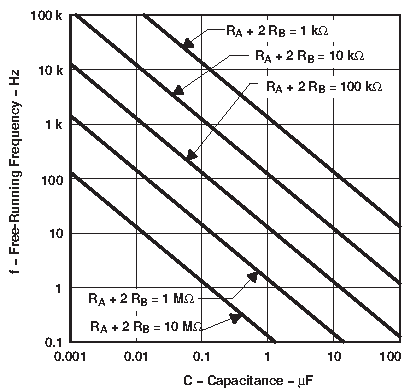
\includegraphics[scale=1]{Graphics/VHDL/Practice 2/GRAPHICS/555/GRAPHS/DATASHEETS/ASTABLE_FREQ.pdf}
        \captionof{figure}{555 Astable Freq. Chart. ~\autocite{555_DS}}
        \label{fig:ASTABLE_FREQ}
    \end{minipage}
    \hfill
    \begin{minipage}[c]{0.49\textwidth}
        \centering
            \begin{align*}
                t_H &= 0.693 \cdot (R_1 + R_2) \cdot C_1& \\
                t_L &= 0.693 \cdot (R_2) \cdot C_1& \\
                T &= 0.693 \cdot (R_1 + 2\cdot R_2) \cdot C_1& \\
            \end{align*}
            
            \vspace{1.5cm}
    \end{minipage}
\end{minipage}

    
\subsubsection{Monostable 555}

The 555 timer can also be used as a \textbf{Monostable Multivibrator} following the circuit down below. 

\begin{figure}[H]
    \centering
    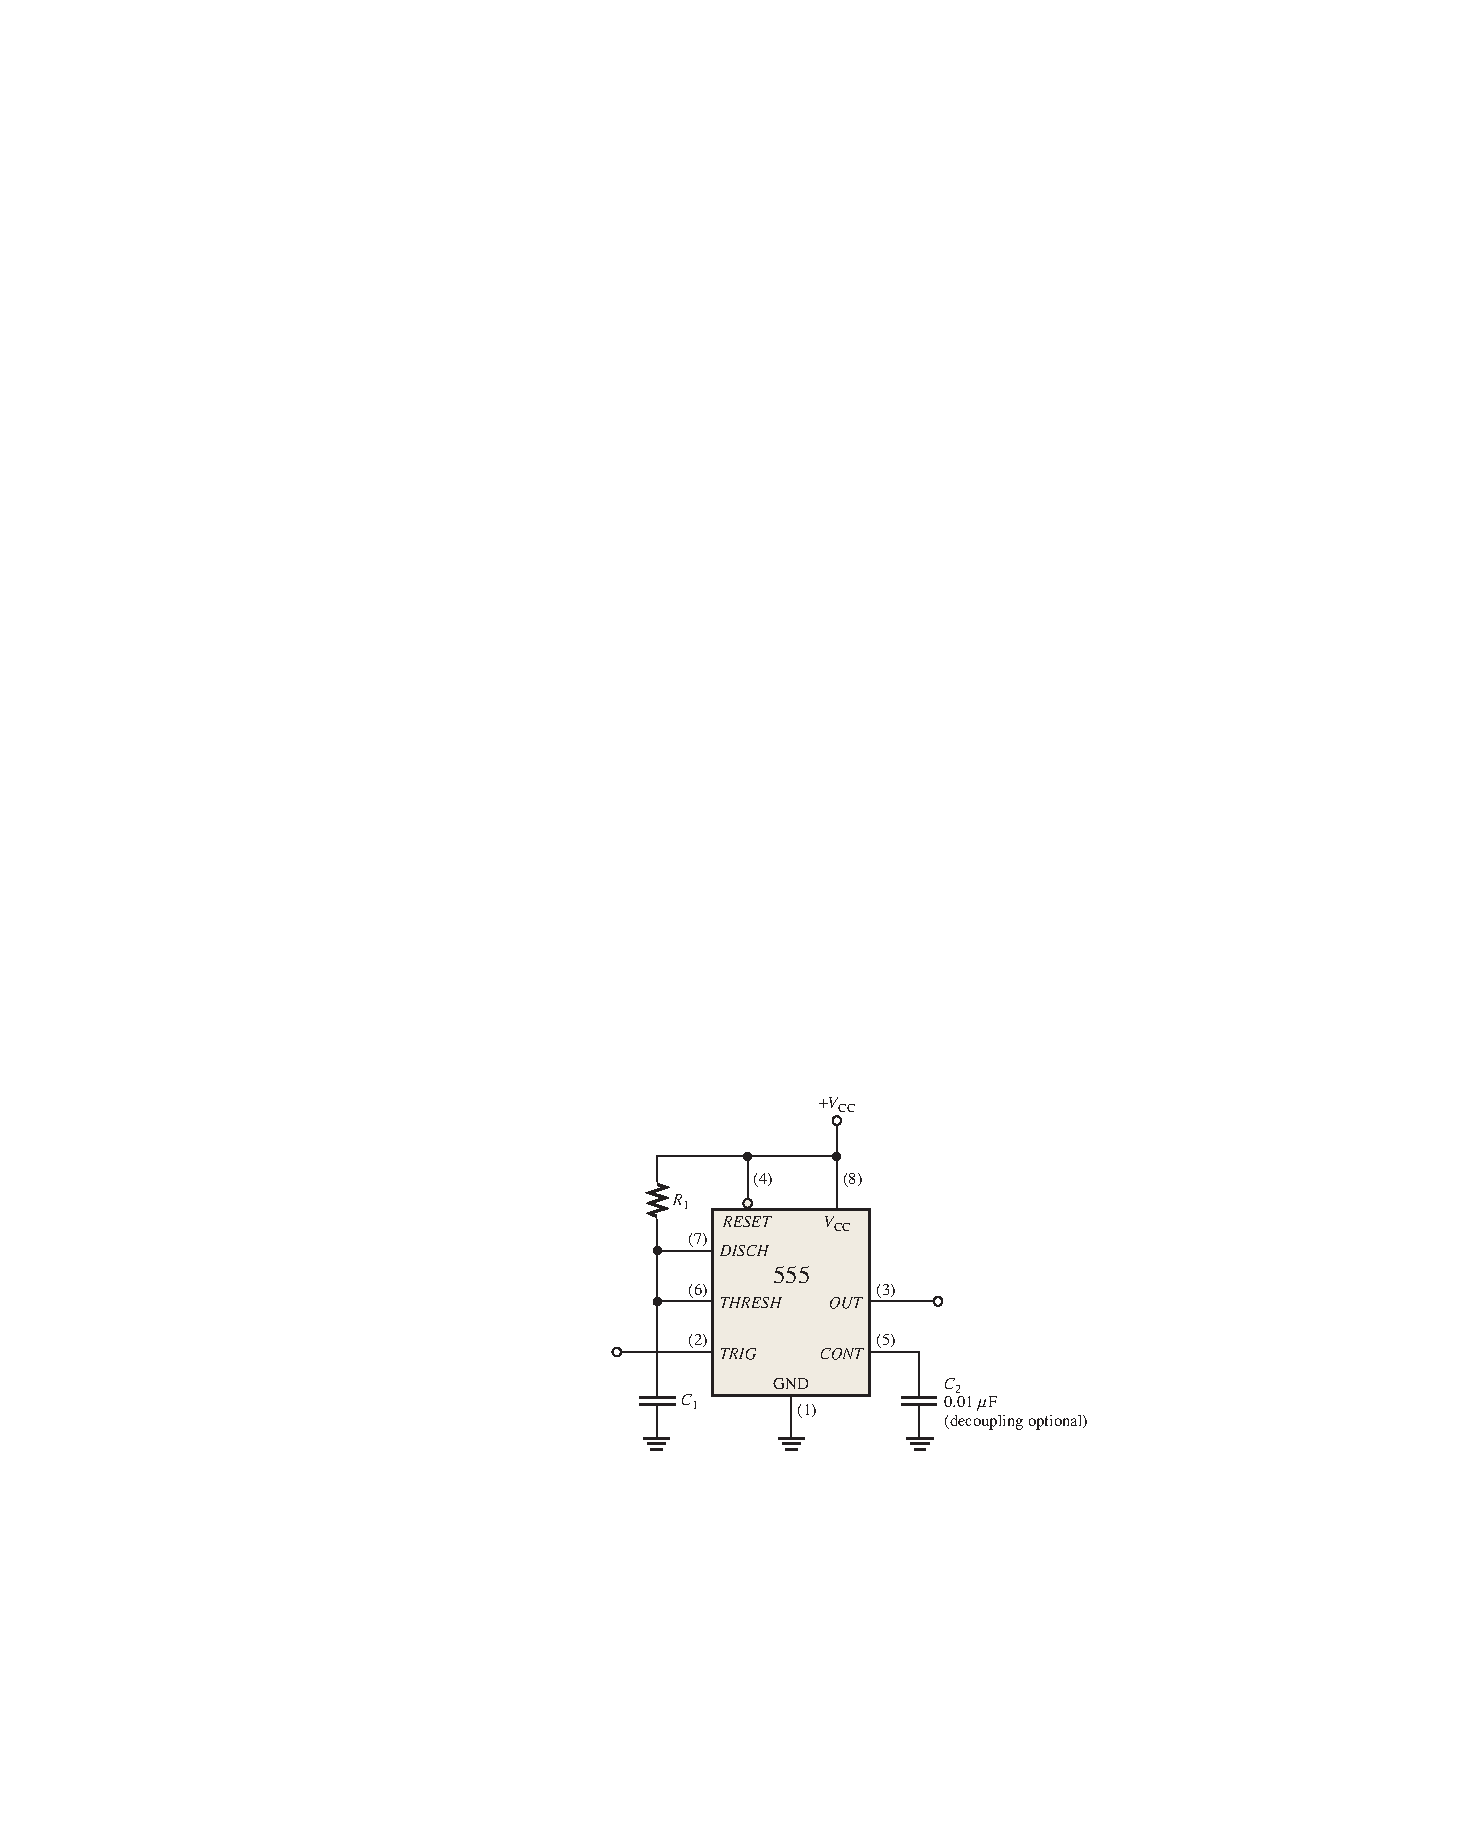
\includegraphics[scale = 1]{Graphics/VHDL/Practice 2/GRAPHICS/555/GRAPHS/MODES/MONOSTABLE.pdf}
    \caption{555 timer connected as an monostable multivibrator (One-shot). ~\autocite{FLOYD}}
    \label{fig:MONOSTABLE}
\end{figure}

As per the other configuration, the duration of the pulse $\mathbf{t_{p}}$ or $\mathbf{t_{w}}$ can be determined by the next equation:

\begin{equation*}
    t_{p} = 1.1 \cdot R_1 \cdot C_1
\end{equation*}

For this configuration, the trigger is a NGP (Negative-going pulse). In the manufacturer's datasheet we can find a chart similar to the last one: \medskip

\begin{figure}[H]
    \centering
    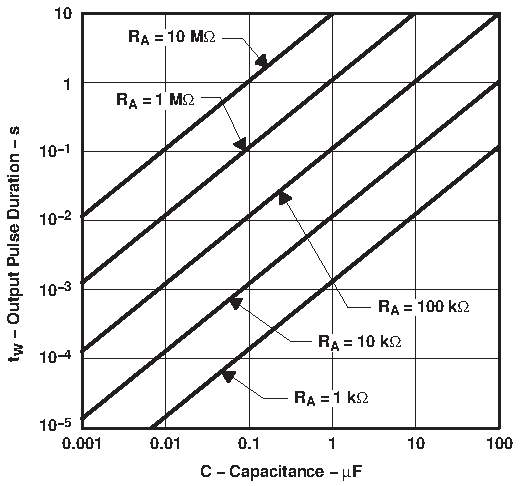
\includegraphics[scale = 0.8]{Graphics/VHDL/Practice 2/GRAPHICS/555/GRAPHS/DATASHEETS/MONOSTABLE_FREQ.pdf}
    \caption{555 timer Monostable Frequency Chart. ~\autocite{555_DS}}
    \label{fig:MONOSTABLE_FREQ}
\end{figure}

\clearpage


\subsection{Exercise 1: 555 as Astable Multivibrator}

\textit{Design an astable multivibrator by using 555 timer with C = 10 nF, $R_1$ = 10 k$\Omega$ y $R_2$ = 10 k$\Omega$. Calculate theoretically the value of $t_H$ (high level semi period), T (period) and DC\% (duty cycle).}\medskip

\textit{Draw and simulate the circuit. Obtain the graphics of the outputs and between the pins of the capacitor. Measure the values of $t_H$ (high level semi period), T (period) and DC\% (duty cycle).}\bigskip

\textbf{\large Answer to Exercise 1:}\medskip

Using the equations listed in \ref{fig:ASTABLE_FREQ} and \ref{fig:DUTY}, obtaining what we are asked is rather simple:

\vspace{-.5cm}

\begin{align*}
    \mathbf{t_H} &= 0.693 \cdot (R_1 + R_2) \cdot C_1 = 0.693 \cdot (10k\Omega + 10k\Omega) \cdot 10\si\nano \text{F} = \mathbf{138.6 \, \textbf{\si\micro s}}
    \\
    \mathbf{t_L} &= 0.693 \cdot (R_2) \cdot C_1 = 0.693 \cdot (10k\Omega) \cdot 10\si\nano \text{F} = \mathbf{69.3 \, \textbf{\si\micro s}}
    \\
    \mathbf{T} &= t_L + t_H = \mathbf{207.9 \, \si\micro \text{s}}
    \\
    \mathbf{D} &= \frac{t_H}{t_H + t_L} \cdot 100= \frac{\mathbf{138.6 \, \si\micro \text{s}}}{\mathbf{138.6 \, \si\micro \text{s} + \mathbf{69.3 \, \textbf{\si\micro s}}}} \cdot 100 = \mathbf{66.6 \, \text{\%}}
\end{align*}\medskip

We are also asked to simulate the circuit. To do this we will make use of ISIS Proteus, as we have done in the past. 

\begin{figure}[H]
    \centering
    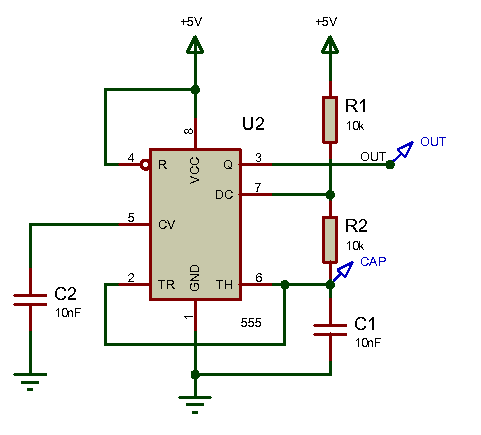
\includegraphics[scale = 1.1]{Graphics/VHDL/Practice 2/GRAPHICS/555/GRAPHS/PROTEUS/ASSEMBLY/555_ASTABLE_10K_ASSEMBLY.PDF}
    \caption{Proteus assembly of the first subsection with $R_2 = 10k \Omega$.}
    \label{fig:555_ASTABLE_10K_ASSEMBLY}
\end{figure}

\clearpage

To check the output, we will employ the Analogue Analysis tool:

\begin{figure}[H]
    \centering
    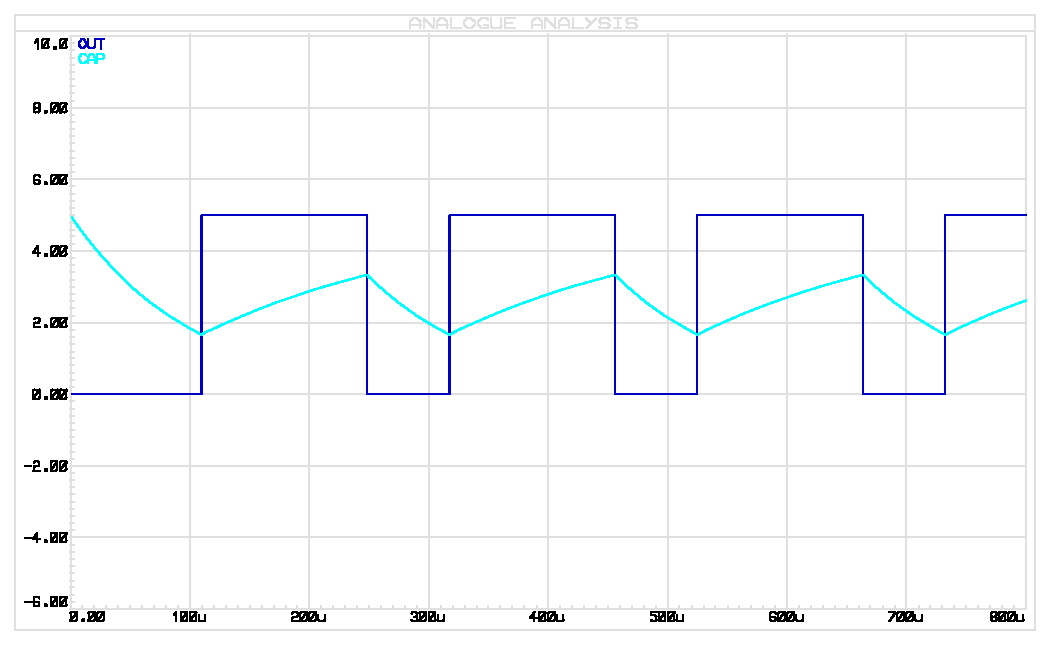
\includegraphics[scale = 0.75]{Graphics/VHDL/Practice 2/GRAPHICS/555/GRAPHS/PROTEUS/ANALOGUE/555_ASTABLE_ANALOGUE_10K.PDF}
    \caption{Analogue Analysis of circuit with $R_2 = 10k \Omega$.}
    \label{fig:555_ASTABLE_ANALOGUE_10K}
\end{figure}


Using the cursors, we can measure the required parameters:

\begin{equation*}
    \mathbf{t_H} = \mathbf{207 \, \si\micro \text{s}} \quad
    \mathbf{t_L} = \mathbf{69 \, \si\micro \text{s}} \quad
    \mathbf{T} = \mathbf{207 \, \si\micro \text{s}} \quad
    \mathbf{D} =  \mathbf{66.6 \, \text{\%}}
\end{equation*}\medskip

As we can see, they match the calculations perfectly since proteus doesn't take into account the tolerances of the different components. The same simulation in NI Multisim yields vastly different results, due to its mathematical models of components being more accurate.\medskip

\clearpage

The exercise now asks us to change the value of $R_2$ to $100k\Omega$ and measure the same parameters. After following the same procedure, we obtain these results:

\begin{figure}[H]
    \centering
    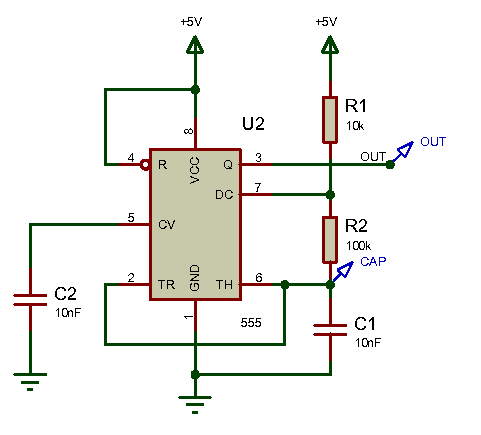
\includegraphics[scale = 1.1]{Graphics/VHDL/Practice 2/GRAPHICS/555/GRAPHS/PROTEUS/ASSEMBLY/555_ASTABLE_100K_ASSEMBLY.PDF}
    \caption{Proteus assembly of the second subsection with $R_2 = 100k \Omega$.}
    \label{fig:555_ASTABLE_100K_ASSEMBLY}
\end{figure}

\begin{figure}[H]
    \centering
    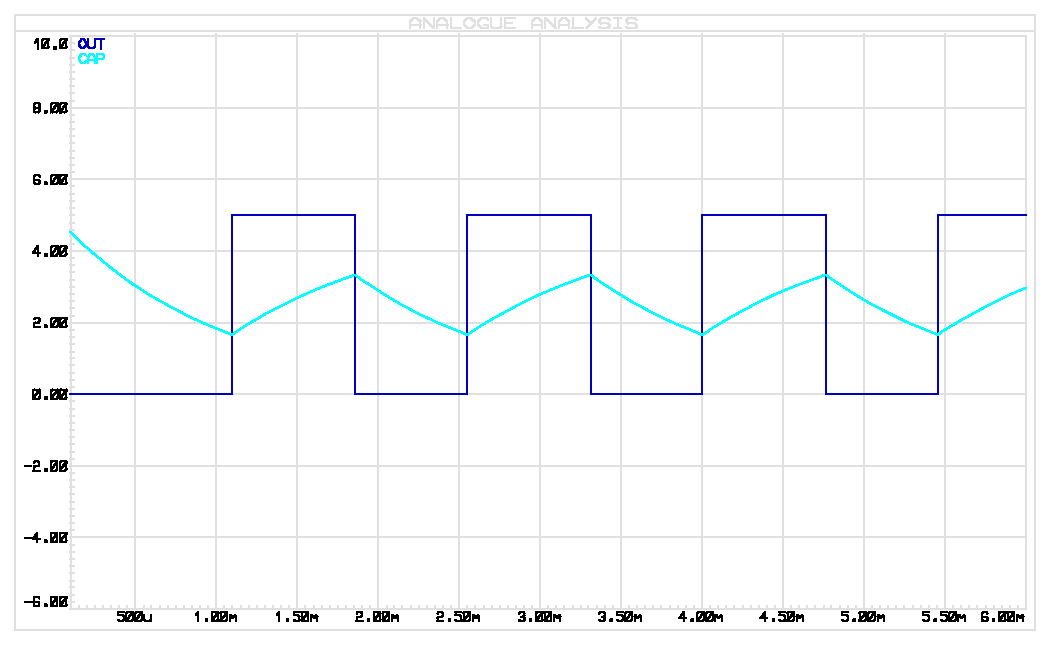
\includegraphics[scale = 0.75]{Graphics/VHDL/Practice 2/GRAPHICS/555/GRAPHS/PROTEUS/ANALOGUE/555_ASTABLE_ANALOGUE_100K.PDF}
    \caption{Analogue Analysis of circuit with $R_2 = 100k \Omega$.}
    \label{fig:555_ASTABLE_ANALOGUE_100K}
\end{figure}

\vspace{-.4cm}

\begin{equation*}
    \mathbf{t_H} = \mathbf{762 \, \si\micro \text{s}} \quad
    \mathbf{t_L} = \mathbf{693 \, \si\micro \text{s}} \quad
    \mathbf{T} = \mathbf{1455 \, \si\micro \text{s}} \quad
    \mathbf{D} =  \mathbf{52.37 \, \text{\%}}
\end{equation*}
\clearpage


The exercise finally asks us to add a diode in parallel with $R_2$ and measure the same parameters. After following the same procedure, we obtain these results:

\begin{figure}[H]
    \centering
    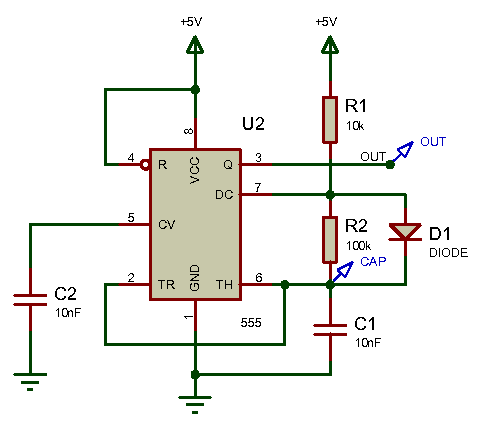
\includegraphics[scale = 1.1]{Graphics/VHDL/Practice 2/GRAPHICS/555/GRAPHS/PROTEUS/ASSEMBLY/555_ASTABLE_100K_DIODE_ASSEMBLY.PDF}
    \caption{Proteus assembly of the third subsection with $R_2 = 100k \Omega$ and a diode in parallel.}
    \label{fig:555_100K_DIODE}
\end{figure}


\begin{figure}[H]
    \centering
    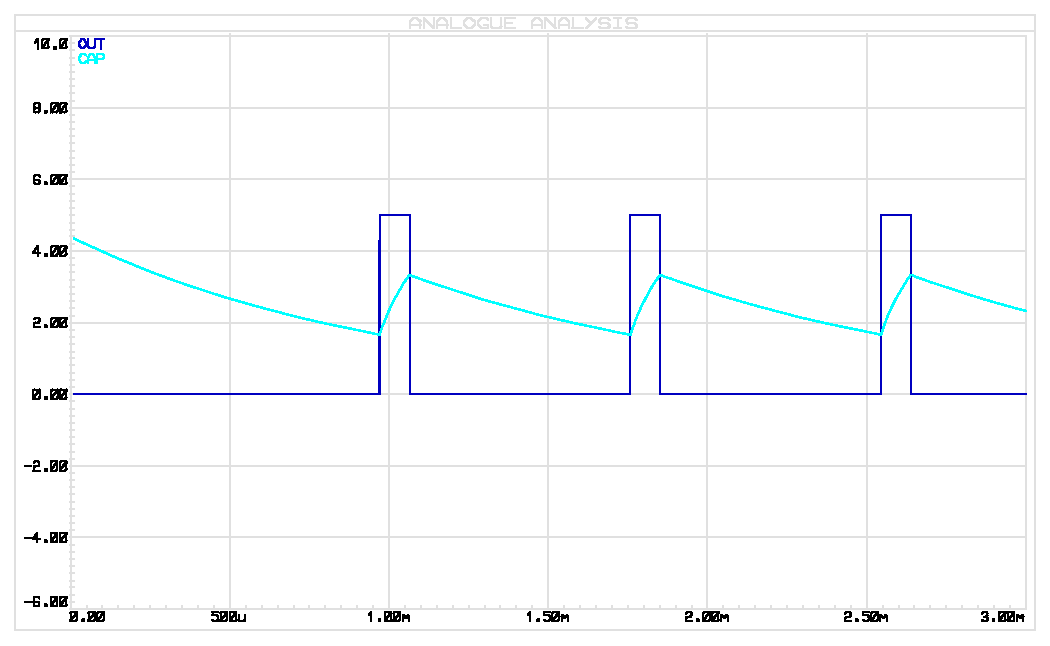
\includegraphics[scale = 0.8]{Graphics/VHDL/Practice 2/GRAPHICS/555/GRAPHS/PROTEUS/ANALOGUE/555_ASTABLE_ANALOGUE_100K_DIODE.PDF}
    \caption{Analogue Analysis with $R_2 = 100k\Omega$ and Diode in parallel.}
    \label{fig:555_ANALOGUE_100K_DIODE}
\end{figure}

\vspace{-.4cm}

\begin{equation*}
    \mathbf{t_H} = \mathbf{98 \, \si\micro \text{s}} \quad
    \mathbf{t_L} = \mathbf{690 \, \si\micro \text{s}} \quad
    \mathbf{T} = \mathbf{788 \, \si\micro \text{s}} \quad
    \mathbf{D} =  \mathbf{12.44 \, \text{\%}} 
\end{equation*}


\subsection{Exercise 2: 555 as Monostable Multivibrator}

In this exercise we are asked to design a one-shot multivibrator (Figure \ref{fig:MONOSTABLE} )using a 555 timer, a 10 \si\micro F capacitor and a $100k\Omega$ resistor. As a reminder, the duration of the pulse of a 555 monostable can be obtained using this equation:

\begin{equation*}
    t_{p} = 1.1 \cdot R_1 \cdot C_1 = 1.1 \cdot 100k\Omega \cdot 10 \si\micro \text{F} = 1.10 \text{s}
\end{equation*}


\begin{figure}[H]
    \centering
    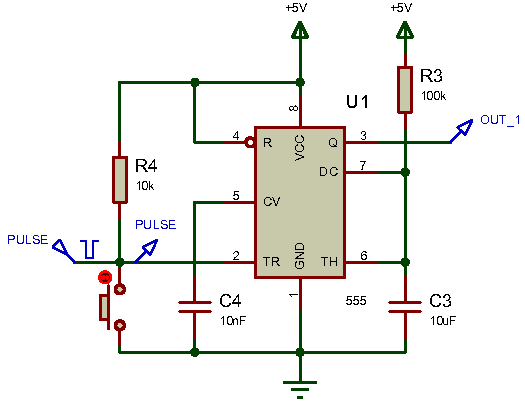
\includegraphics[scale = 1.045]{Graphics/VHDL/Practice 2/GRAPHICS/555/GRAPHS/PROTEUS/ASSEMBLY/555_MONO_ASSEMBLY.PDF}
    \caption{Proteus assembly of a Monostable Multivibrator}
    \label{fig:555_MONO_ASSEMBLY}
\end{figure}


\begin{figure}[H]
    \centering
    
    \ifnum\value{ANIMATION}=1 {
        \animategraphics[controls,loop,scale=0.75]{1}{Graphics/VHDL/Practice 2/GRAPHICS/ANIMATION/555/555_MONO_ANALOGUE_F}{0}{1}
    } 
    \else {
        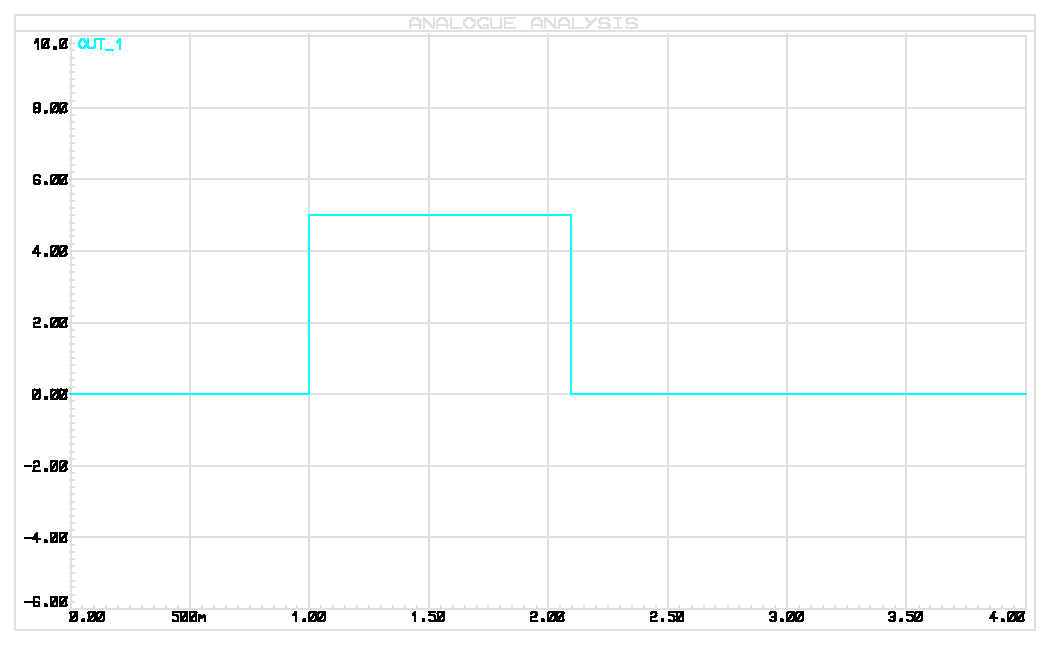
\includegraphics[scale=0.75]{Graphics/VHDL/Practice 2/GRAPHICS/ANIMATION/555/555_MONO_ANALOGUE_F1.PDF}
    }\fi
    
    \caption{Analog Analysis of a Monostable Multivibrator.}
    \label{fig:555_MONO_ANALOGUE}
\end{figure}

\clearpage


\section{Laboratory Lecture 3: Stepper Motor Controller}
\label{sec:STEPPER_MOTOR}

\subsection{Introduction}

The aim of this practice is to go over the basics of how to control a stepper motor. A stepper motor is a brushless DC electric motor that divides a full rotation in several small increments or \textit{steps}. By providing power to its coils in a specific way, we can control the position of the shaft.\medskip

Stepper motors can be unipolar or bipolar. Unipolar Stepper motors are very similar to Bipolar Stepper Motors, but are manufactured with a central tap that connects back to the power source, essentially splitting each coil into two smaller coils that can be powered independently. If required, the central tap can also be left disconnected, allowing the Unipolar Stepper Motor to be converted into a Bipolar configuration.\medskip

Bipolar Stepper Motors do not feature a central tap for dividing their solenoid coils. This makes their internal wiring slightly less complex than that of a Unipolar Motor.

\vspace{0.3cm}

\begin{figure}[H]
    \centering
    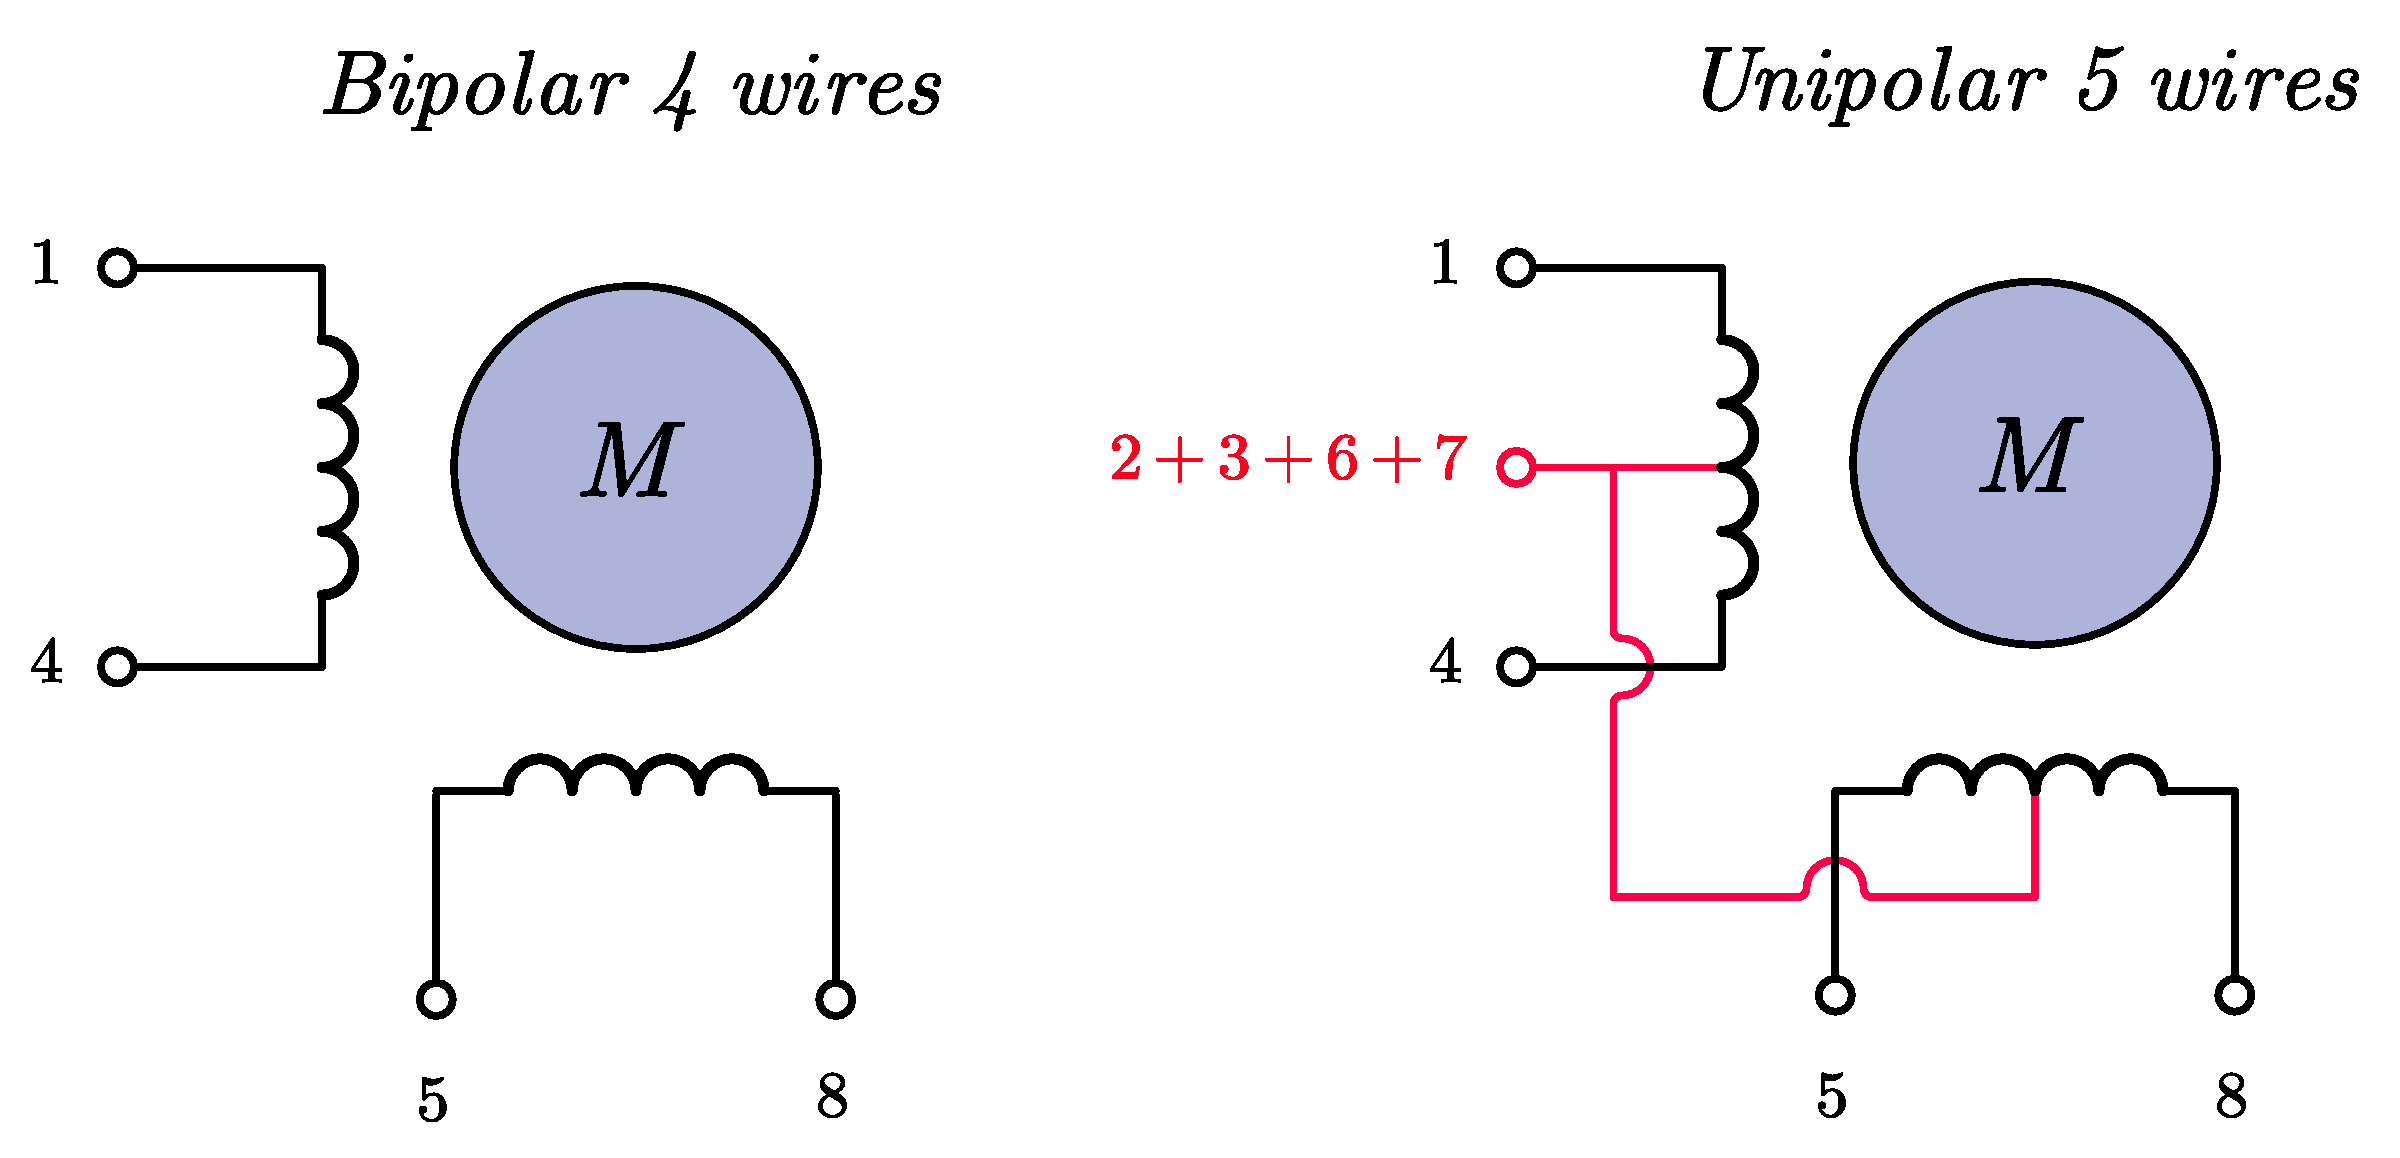
\includegraphics[scale = 0.24]{Graphics/VHDL/Practice 3/GRAPHICS/STEPPER_TYPES.pdf}
    \caption{Bipolar vs. Unipolar configurations.}
    \label{fig:STEPPER_TYPE}
\end{figure}

\clearpage

\subsection{Exercise 1: Stepper Motor Controller}

In this practice we will use the Bipolar type, in particular a NEMA 17 motor. To control it we will use a special driver, the L293D, which is basically an array or darlington transistors, in half-H configuration,  whose main objective is to take care of switching the high currents that the motors require. 

\vspace{0.3cm}

\begin{figure}[H]
    \centering
    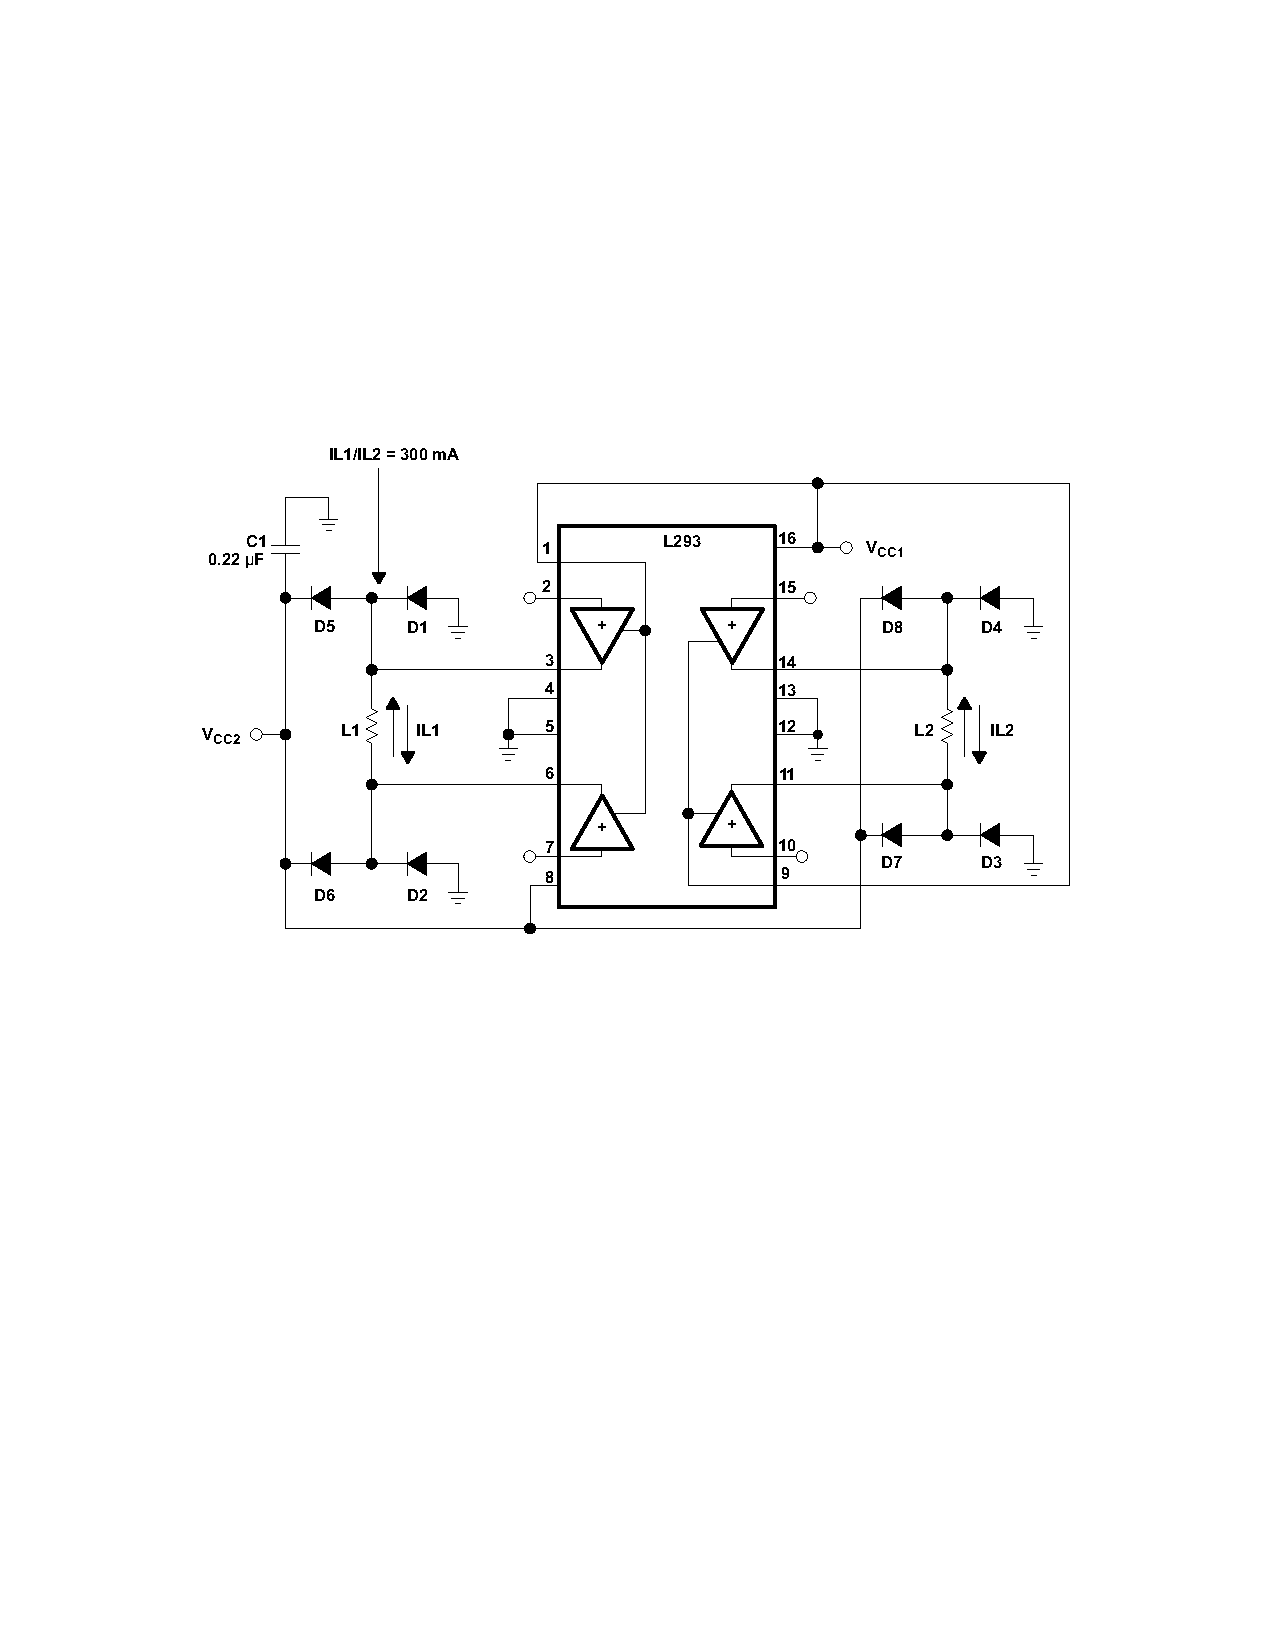
\includegraphics[scale = 0.85]{Graphics/VHDL/Practice 3/GRAPHICS/DATASHEETS/L293D_INTERNAL.pdf}
    \caption{L293D Bipolar Stepper Controller. ~\autocite{L293D}}
    \label{fig:L293D}
\end{figure}

To control said driver, we will make us of the SPLD that we have been using since the beginning, the GAL22V10C and some basic VHDL code. In order to make the shaft spin in a controlled manner, we have to take into account the phase current waveforms, i.e. the pulses that we have to send to the driver to cause a step change and the order in which they must be sent. This information can be seen below:

\vspace{0.3cm}

\begin{table}[ht]
    \centering
        \begin{tabular}[t]{lcccc}
            \toprule
            &\textbf{Step}&\textbf{Full-Step [1.8\textdegree]}&\textbf{Wave-Step [1.8\textdegree]}&\textbf{Half-Step [0.9\textdegree]}\\
            \midrule
            & 0 & 1010 & 1000 & 1010\\
            & 1 & 1001 & 0001 & 1000\\
            & 2 & 0101 & 0100 & 1001\\
            & 3 & 0110 & 0010 & 0001\\
            & 4 &      &      & 0101\\
            & 5 &      &      & 0100\\
            & 6 &      &      & 0110\\
            & 7 &      &      & 0010\\
            \bottomrule
        \end{tabular}
        \caption{Phase Current Waveforms. ~\autocite{SLIDES_3}}
        \label{table: PHASE_CURRENT_WAVEFORMS}
\end{table}

\subsubsection{VHDL Code}

As we have seen in Table \ref{table: PHASE_CURRENT_WAVEFORMS}, there are 3 different ways in which we can control the rotation of the stepper motor, namely, full-step, wave-step and half-step. Each of them present advantages and disadvantages. For instance, \textit{Half-Steps} can deliver a higher precision, since every step only spins the shaft 0.9\textdegree as opposed to \textit{full-step} and \textit{wave-step}, which spin it 1.8\textdegree. This increase in performance reduces the output torque significantly, so there is a clear trade-off between both variables that one must consider. In addition to this, \textit{Wave-step} mode is more visually appealing, as the transitions between states are not as choppy as with the other ones.\medskip

Due to the limitations that the GAL22V10C possesses, it is not possible to fit the 3 control modes in the same SPLD. That's why we have developed 3 different codes, one for each, that can be seen below:

\paragraph{Full Step}
\label{sec:FULL_STEP}

\inputcode{CODES/VHDL/Practice_3/Full_Step.vhd}


As we have previously mentioned, \textit{Full Step} phase control provides the highest torque of all, though the transitions tend to look quite choppy. This mode and the \textit{Wave Step} one provide a maximum accuracy of 1.8\textdegree \, per step, which means that a full 360\textdegree \, rotation would require 200 steps.\medskip

The code that we have included moves the shaft one step (forwards or backwards) whenever a \textit{PGT} occurs. This indicates that the process is synchronous. Besides, we can also find a direction pin which changes the direction of the spin when a positive signal is applied to it.

\paragraph{Wave Step}

\inputcode{CODES/VHDL/Practice_3/Wave_Step.vhd}

This code describes the \textit{Wave Step} phase control sequence. Wave Stepping is usually used when the smoothness of the output rotation is important. As per the last mode, this mode has a high torque but its trade-off is a reduction in its accuracy. \medskip

The rest of the code remains the same as the last one.

\paragraph{Half Step}

\inputcode{CODES/VHDL/Practice_3/Half_Step.vhd}


In addition, we can find the \textit{Half Step} phase control sequence. As we can see, this code is longer than the last 2 codes. This is due to the fact that it has some intermediate states which help smooth out the rotation by getting rid of most of the chopping that characterizes the latter.


\subsubsection{Proteus Simulation and Assembly}

After discussing the code, we will move on to the simulation of the circuit. For this we will use ISIS Proteus once again. Even though Figure \ref{fig:L293D} may look cumbersome, in actuality, we only have to connect the 2 coils to the driver's output and the 4 direction pins to its inputs following this fashion:\medskip

\begin{figure}[H]
    \centering
    
    \ifnum\value{ANIMATION}=1 {
        \animategraphics[controls,loop,scale=0.8]{1}{Graphics/VHDL/Practice 3/GRAPHICS/ANIMATION/F}{0}{8}
    } 
    \else {
        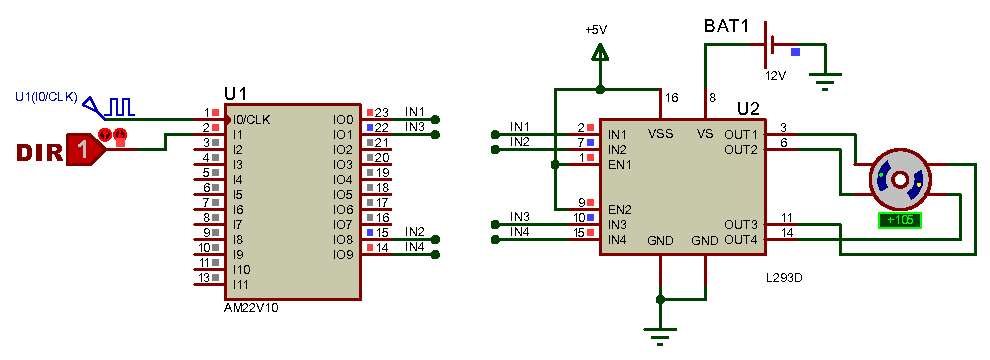
\includegraphics[scale=0.8]{Graphics/VHDL/Practice 3/GRAPHICS/ANIMATION/F5.PDF}
    }\fi
    
    \caption{Stepper with rotation direction control.}
    \label{fig:STEPPER_ROTATION}
\end{figure}

The I/O pins that we used are the ones that the the compiler assigned by default. They are displayed in the Chip Report (Figure \ref{fig:CHIP_REPORT}).\medskip

Assembling the circuit is just a matter of manually connecting everything following the schematic of Figure \ref{fig:STEPPER_ROTATION}. To provide a clock signal we have used a signal generator which output has been set to a TTL level, 0 to 5V, and its frequency to 1 Hz.  

\clearpage
\section{Laboratory Lecture 4: Stepper Motor Controller}

The main objective of this practice is to understand the fundamentals of Finite State Machines and their main applications. We will then use the knowledge that we have acquired to build a stepper motor controller which will be controlled by a rotary encoder.

\subsection{Introduction}

\subsubsection{Finite State Machines}

Before diving into the practice, we must firstly define what a Finite State Machine. In essence, a FSM is a machine that makes predictable transitions through a sequence of states, based on external inputs and the current state of the machine. In digital electronics, the timing of the transition of the machine from one state to another is controlled by a register and a system clock, while the next state of the machine is determined by a combination of logic gates and embedded memory. The number of states, as the name suggests can be assumed to be finite. ~\autocite{FSM} \medskip

Two basic types of state machines are the Moore and the Mealy. The Moore state machine is one where the outputs depend only on the internal present state. The Mealy state machine is one where the outputs depend on both the internal present state and on the inputs. ~\autocite{FLOYD} \medskip

We can see and example of these type of machines here:


\begin{figure}[H]
    \centering
    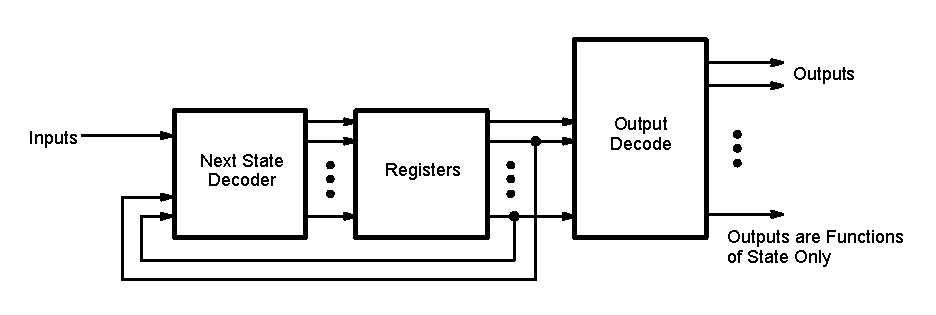
\includegraphics[width = \textwidth]{Graphics/VHDL/Practice 4/MOORE.pdf}
    \caption{Moore State Machine Operation Diagram ~\autocite{AMD}}
    \label{fig:MOORE}
\end{figure}

\vspace{-0.3cm}

\begin{figure}[H]
    \centering
    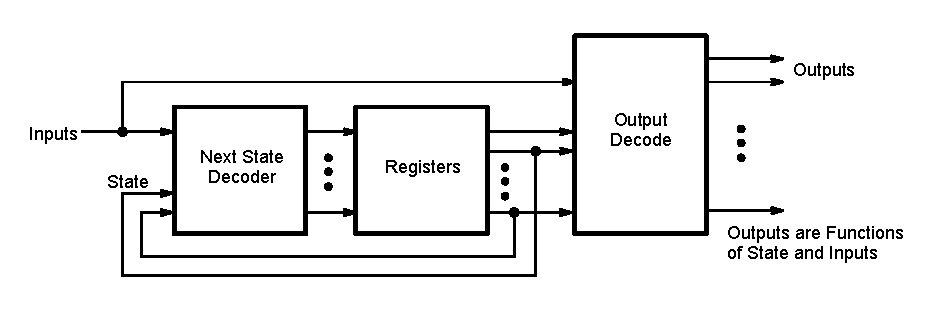
\includegraphics[width = \textwidth]{Graphics/VHDL/Practice 4/MEALY.pdf}
    \caption{Mealy State Machine Operation Diagram ~\autocite{AMD}}
    \label{fig:MEALY}
\end{figure}


To represent both types of machines, a State Diagram is used. Normally, state diagrams are composed of bubbles, which indicate the different states, and arrows, that indicate the transitions.\medskip

In the following example we will implement a FSM that recognizes the sequence "10" using both type of machines.

\begin{figure}[H]
    \centering
    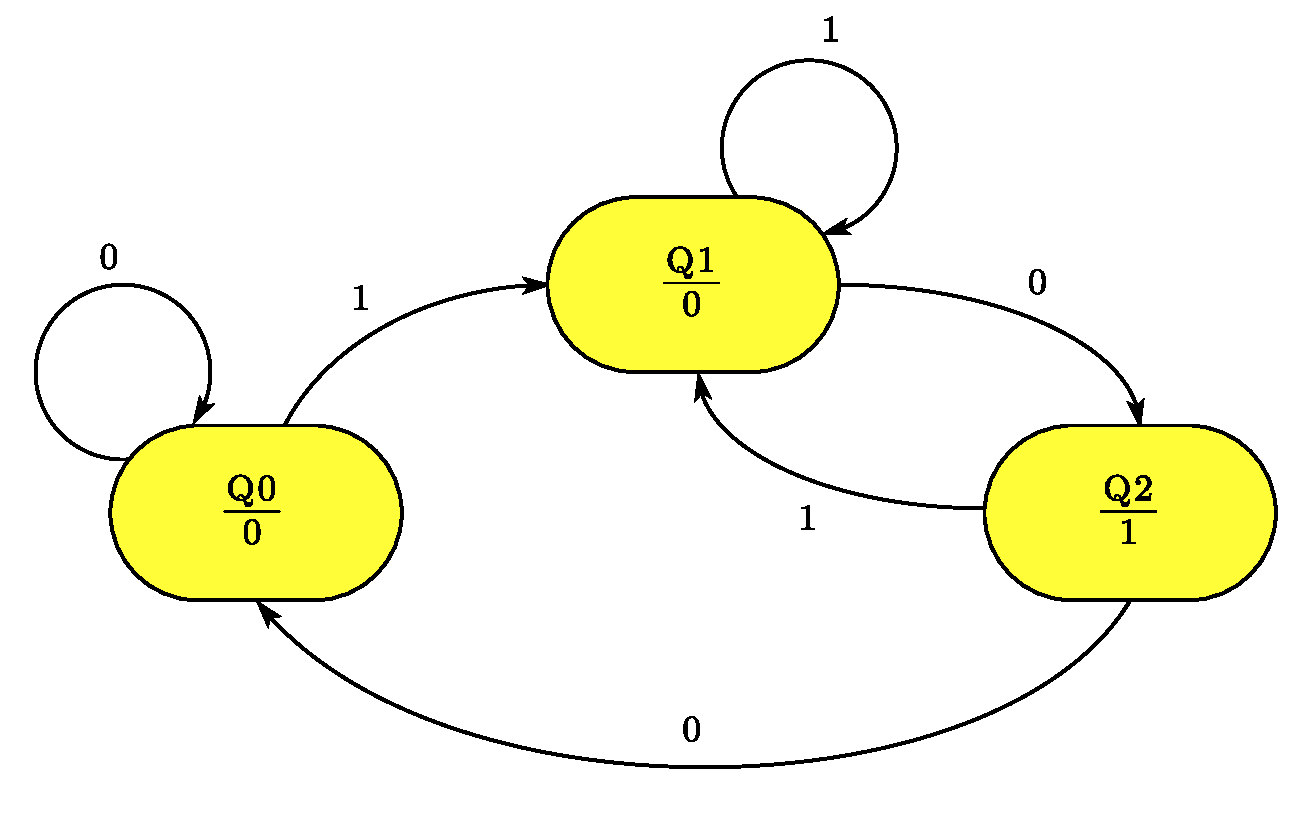
\includegraphics[scale = 0.55]{Graphics/VHDL/Practice 4/MOORE_FSM.pdf}
    \caption{Moore State Machine ~\autocite{SLIDES_4}}
    \label{fig:MOORE}
\end{figure}

For this particular case, \bm{$Q_0$} means \textit{No elements in the sequence observed}, \bm{$Q_1$} means \textit{"1" observed} and \bm{$Q_2$} means \textit{"10" observed}

\vspace{-0.3cm}

\begin{figure}[H]
    \centering
    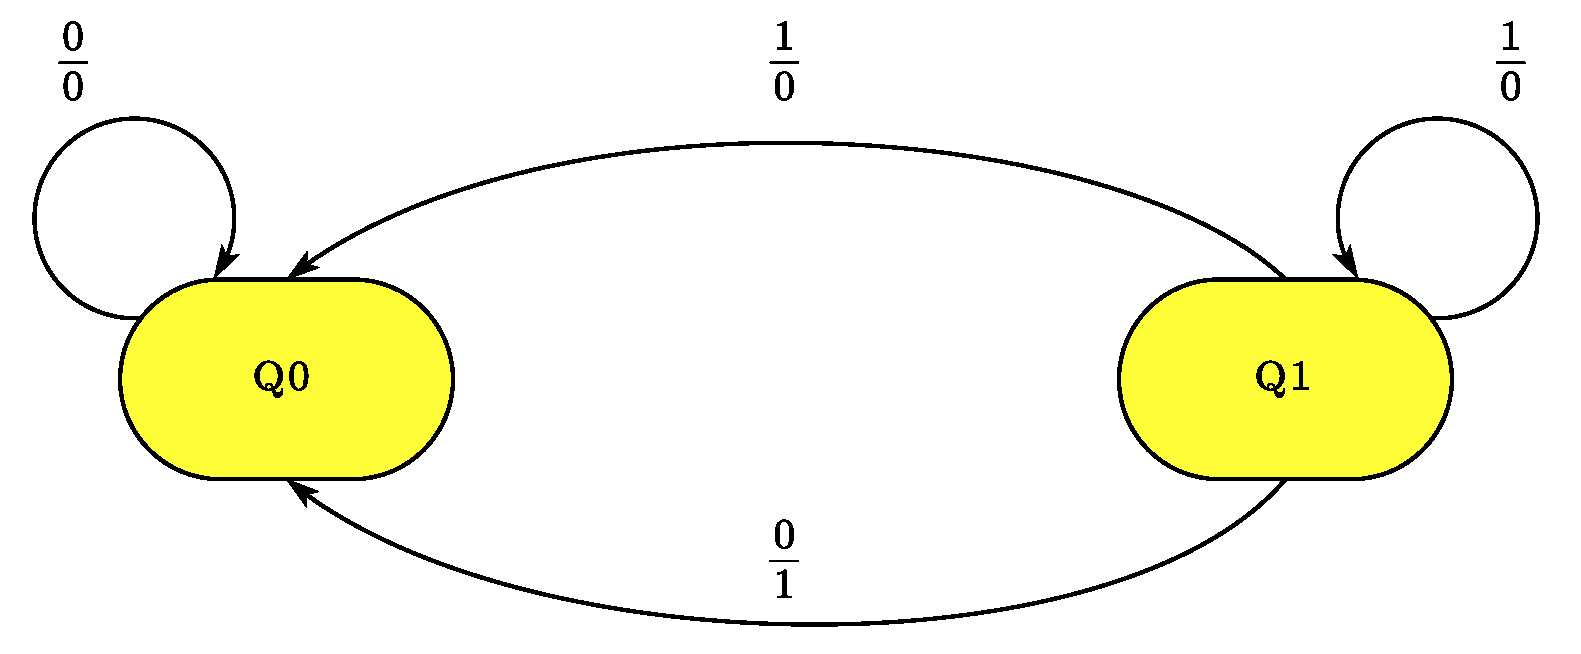
\includegraphics[scale = 0.45]{Graphics/VHDL/Practice 4/MEALY_FSM.pdf}
    \caption{Mealy State Machine ~\autocite{SLIDES_4}}
    \label{fig:MEALY}
\end{figure}

In the latter case, the states mean the same, but as we can seem there is one less state than in the previous one. \bigskip


This brings us to the advantages and disadvantages that both of them have:

\begin{enumerate}
    \item Mealy machines have \textbf{fewer states} and react faster to inputs.
        \begin{itemize}
            \item Outputs are defined in the transitions ($n^2$) rather than in the state itself ($n$).
            \item They react in the same cycle, i.e., they do not need to wait for the clock.
            \item Their outputs may be considerably shorter than the clock cycle, which can pose problems.
            \item Since fewer states than the \textbf{Moore} type are used, the propagation delay time is also shorter.
        \end{itemize}
    \item Moore machines are \textbf{safer} to use.
        \begin{itemize}
            \item Outputs change at clock edge.
            \item In \textbf{Mealy machines}, an input change will cause an output change as soon as the logic is done, which a big problem when two machines are interconnected since asynchronous feedback may occur if one is not careful.
        \end{itemize}
\end{enumerate}

\clearpage

\subsubsection{Incremental encoder}

An incremental encoder is a type of rotary encoder that indicates both the ocurrence and the direction of movement. An encoder of such type does not indicate the absolute position or angle; it only reports changes in position and for each position, the direction of movement. \medskip

They usually have 2 outputs, \textit{A} and \textit{B}, which value changes as the encoder is swept through its range, incrementing the count every time that its shaft changes position.\medskip

\vspace{-0.5cm}

\begin{figure}[H]
    \centering
    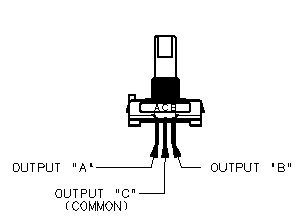
\includegraphics[scale = 1.3]{Graphics/VHDL/Practice 4/ENCODER_DRAWING.pdf}
    \caption{Encoder pinout ~\autocite{ENCODER}}
    \label{fig:ENCODER_PINOUT}
\end{figure}

Incremental encoders output a defined number of pulses per revolution. We can use these pulses to obtain both the angle and the direction of the rotarion since the outputs \textit{A} and \textit{B} are shifted 90\textdegree. This behaviour can be clearly seen in the following graph:\medskip

\begin{figure}[H]
    \centering
    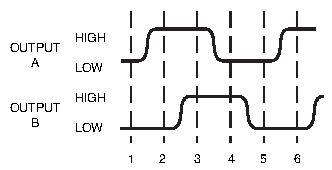
\includegraphics[scale = 1.5]{Graphics/VHDL/Practice 4/ENCODER_POSITION.pdf}
    \caption{Encoder Output States ~\autocite{ENCODER}}
    \label{fig:ENCODER_STATES}
\end{figure}

\clearpage

\subsection{Exercise 1: Motor Control}

Now that we have defined how every part of the system works, we will move onto solving the laboratory lecture itself. \medskip

The first and only exercse states the following:\medskip

\textit{Design a state machine (FSM) that supplies the proper output to a stepper motor according to the position of the incremental encoder. Draw the FSM.} \medskip

\textbf{\large Answer to Exercise 1:}\medskip

As per usual, we will implement the code for the FSM in VHDL and we will program it into a GAL22V10C. \medskip

The VHDL code can be found below:\medskip

\inputcode{CODES/VHDL/Practice_4/ENCODER.vhd}

As we can clearly see in the code, this FSM is of the type Moore, as the outputs update in the states themselves rather than in the transitions. In addition, since the capacity of the GALs is very limited, we have not added an asynchronous nor synchronous reset pin, which could cause problems in other, more complex FSMs.  \medskip

The output signal \textbf{STEPPER} will be connected to the stepper motor driver that we saw in the last practice so as to simulate a similar version of the full-step control mode with fewer states (\textbf{See Subsubsection \ref{sec:FULL_STEP} for more on this})\medskip

The State Diagram that describes this FSM can be found below:

\begin{figure}[H]
    \centering
    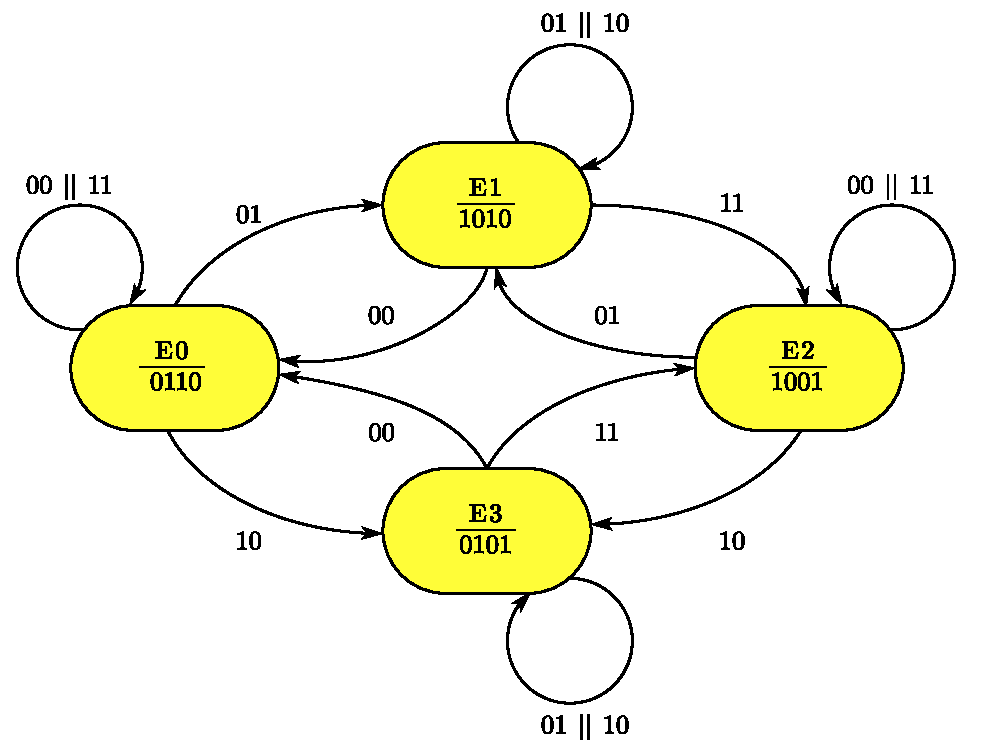
\includegraphics[scale = 0.75]{Graphics/VHDL/Practice 4/EXERCISE_FSM.pdf}
    \caption{Stepper Controller with Incremental Encoder FSM}
    \label{fig:ENCODER_FSM}
\end{figure}

\clearpage

% Clear TOC page

\addtocontents{toc}{\protect\thispagestyle{empty}}

\section{Laboratory Lecture 5: Keypad Control}
\label{sec:KEYPAD_GENERAL}

The aim of this practice is to understand how shift registers work, how to impement them using VHDL and, finally, how to build a keypad-controlled 7-segment display using a ring counter, a specific application of shift registers. This knowledge will be later used to implement more complex systems in further laboratory sessions. 

\subsection{Introduction}

Before delving into the practice itself, we will first go over the basics of shift registers, counters, keypads, and 7-segment displays.

\subsubsection{Shift Registers}

A shift register can be described as an array of flip-flops (\textbf{See Section \ref{sec:FLIP_FLOPS} for more information on this topic}) in which the output of one of connected to the input of the next one. They are mostly used in applications that involve the storage and transfer of data in a digital system.\medskip

A \textbf{register} is a digital circuit with two basic functions: data storage and data movement.
The storage capability of a register makes it an important type of memory device. Figure \ref{fig:D_FLIP_FLOP} illustrates the concept of storing a 1 or a 0 in a D flip-flop. A 1 is applied to the data input as shown, and a clock pulse is applied that stores the 1 by \textit{setting} the flip-flop. When the 1 on the input is removed, the flip-flop remains in the \textit{SET} state, thereby storing the 1. A similar procedure applies to the storage of a 0 by \textit{resetting} the flip-flop, as also illustrated in Figure \ref{fig:D_FLIP_FLOP} ~\autocite{FLOYD}

\begin{figure}[H]
    \centering
    \hspace{0.88cm}
    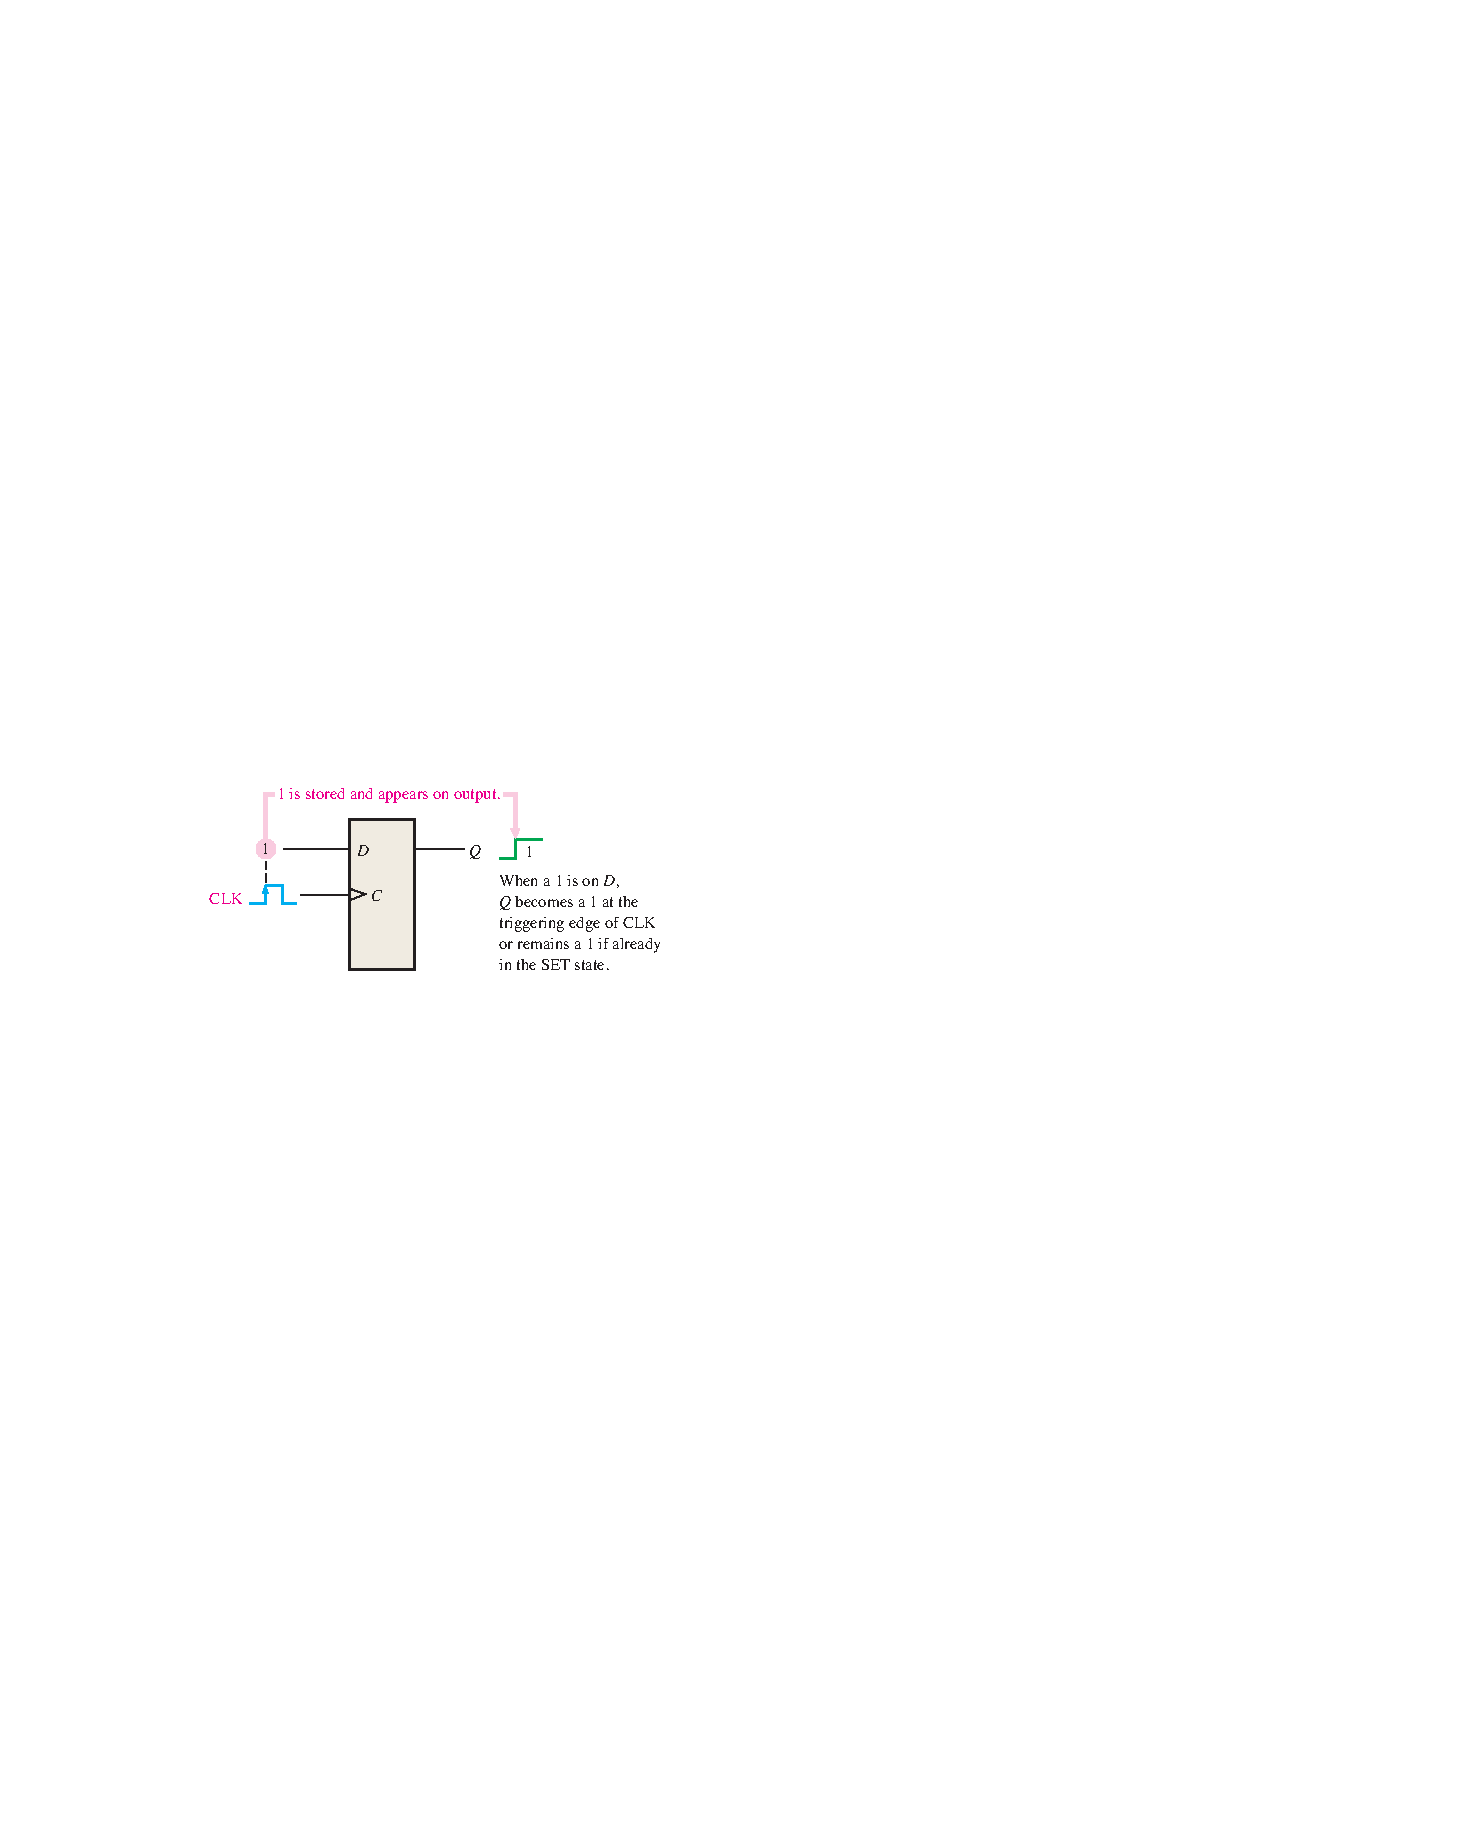
\includegraphics[scale = 1]{Graphics/VHDL/Practice 5/SHIFT_REGISTER_BASICS/D-Latch_Operation_451_1.pdf}
\end{figure}

\begin{figure}[H]
    \centering
    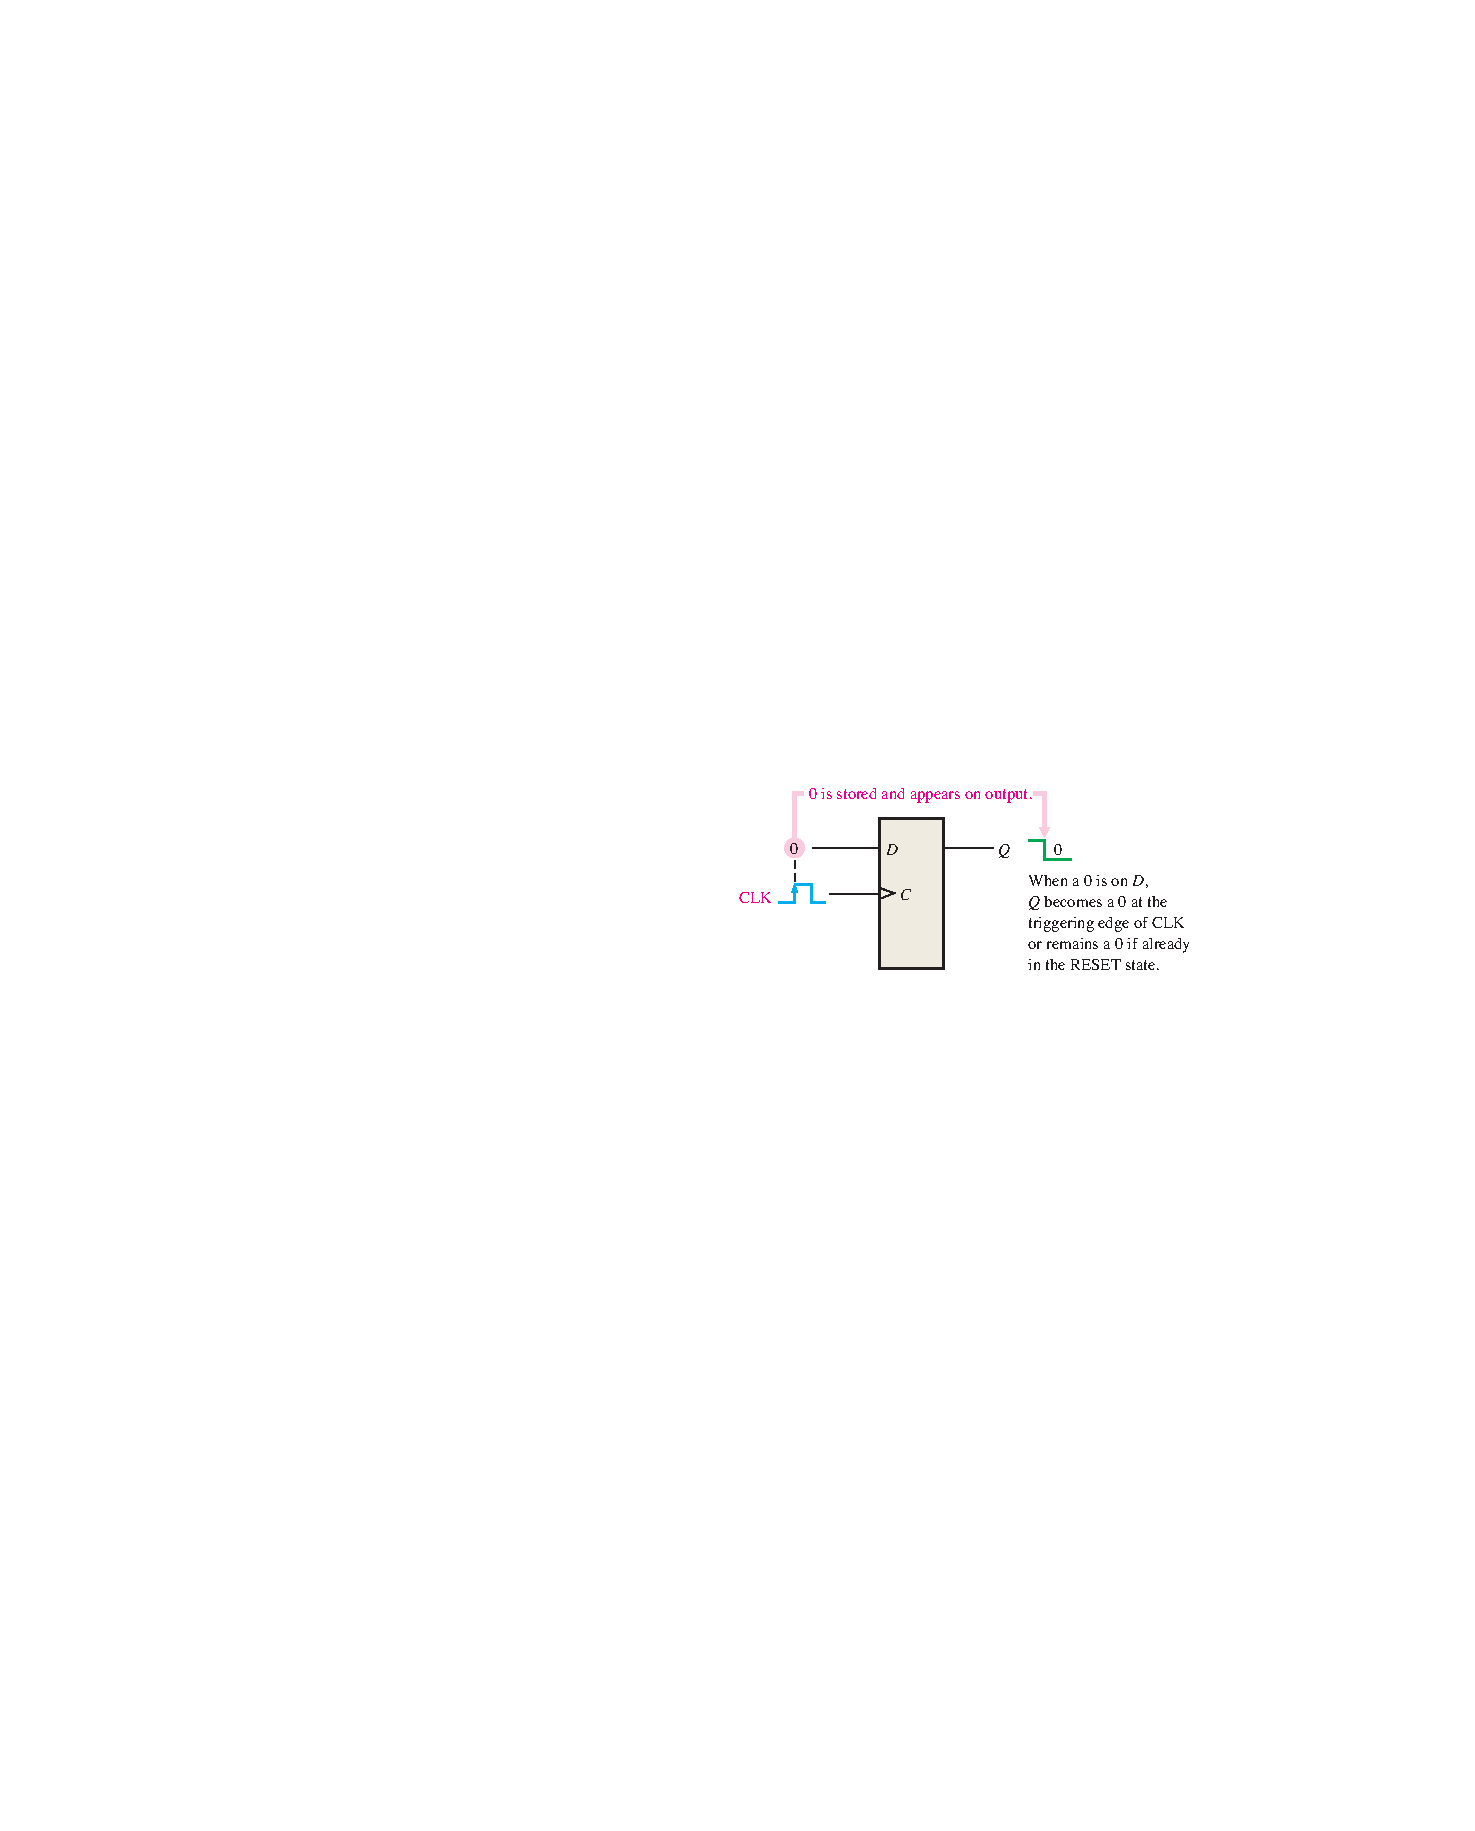
\includegraphics[scale = 1]{Graphics/VHDL/Practice 5/SHIFT_REGISTER_BASICS/D-Latch_Operation_451_2.pdf}
    \caption{D-Flip Flop as a data storage element ~\autocite{FLOYD}}
    \label{fig:D_FLIP_FLOP}
\end{figure}

\clearpage

Depending on the configuration of the flip-flops, the data that they trasmit and store can be \textit{shifted}, or moved, in several ways. We can see this in the illustration attached below:

\begin{figure}[H]
    \centering
    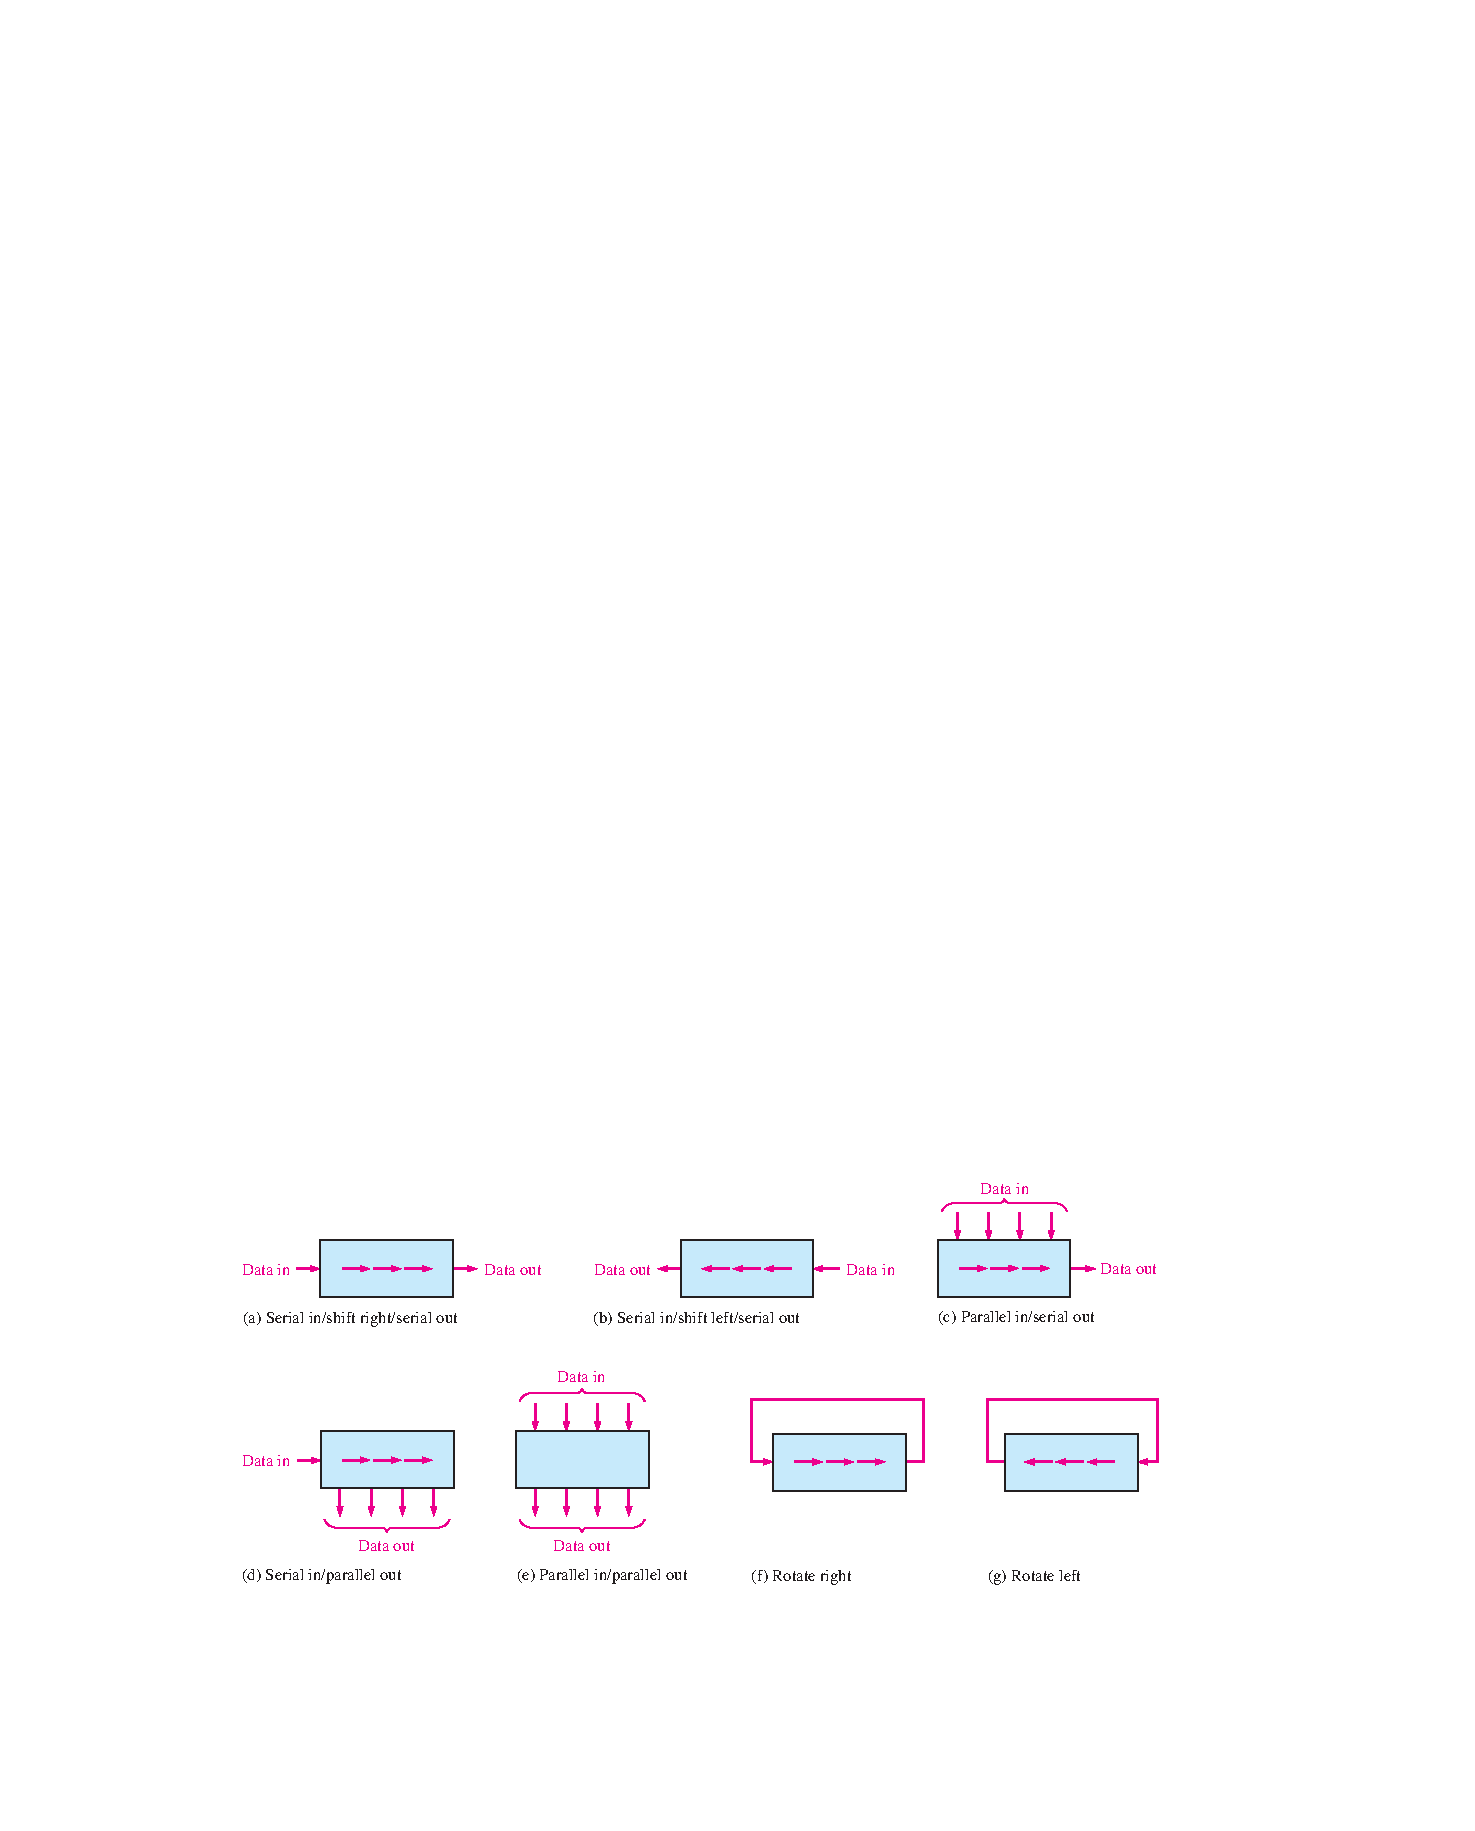
\includegraphics[scale = 0.85]{Graphics/VHDL/Practice 5/SHIFT_REGISTER_BASICS/DATA_TRANSMISSION/Data_Movement_451.pdf}
    \caption{Different types of data transfer ~\autocite{FLOYD}}
    \label{fig:DATA_TRANSFER}
\end{figure}

These different configurations allow us to streamline the transmission and storage of data. By using, for instance, a Parallel-In Serial-Out configuration, we can reduce the amount of wires that are needed to perform a data transmission. Even though a serial transmission is slower than a parallel one, one might argue that for most day to day applications, its speed is enough. Examples of this may include the USB bus, UART, SPI, and I2C communication and so on.\medskip

The opposite also exist, as we can see in Figure \ref{fig:DATA_TRANSFER}. In fact, it is common to use a combination of both transmission methods in order to transfer data reliably and cost effectively, since all of the data packets are transmitted using one wire instead of multiple ones. The only thing that the user must do to obtain the initial parallel data is to \textit{decode} the stream of serial data. To do this a Serial-In Parallel-Out shift register is used. \medskip

\clearpage

We can see an example of this type of data transfer below:

\begin{figure}[H]
    \centering
    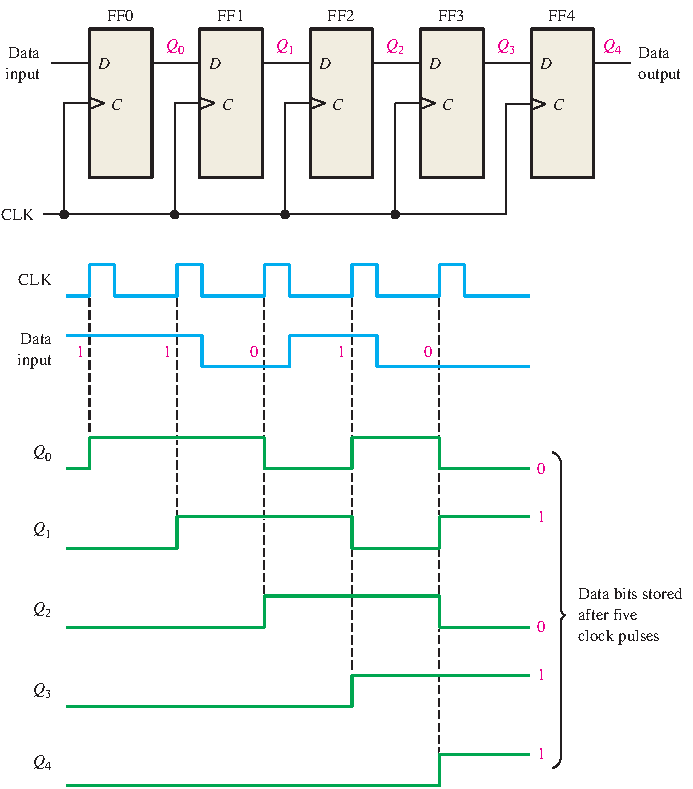
\includegraphics[]{Graphics/VHDL/Practice 5/SHIFT_REGISTER_BASICS/DATA_TRANSMISSION/SIPO_and_Wave.pdf}
    \caption{Serial-In Parallel-Out ~\autocite{FLOYD}}
    \label{fig:SIPO}
\end{figure}

As we can see in the picture, every time that there a PGT occurs, the data in the input in introduced in the first Flip-Flop and the rest of the data skips on place. In this example in particular, after 4 clock cycles, the 4 input data bits are shown in $Q_0 - Q_3$ at the same time, effectively converting serial data into parallel data.\medskip

\clearpage

\subsubsection{Counters}
\label{sec:COUNTERS}

On the other hand, shift registers can also be used to create \textbf{counters}. A shift register counter is basically a shift register with the serial output connected back to the serial input to produce special sequences. These devices are often classified as counters because they exhibit a specified sequence of states.\medskip 

Two of the most common types of shift register counters are the Johnson counter and the Ring counter. The main difference between them is the connection between the output of the last flip flop to the input of the first one. In Ring counters, the output \bm{$Q_{final}$} is directly connected to the input \bm{$D_{initial}$}, whereas in Johnson counters, the output that gets connected to the inpus is the \bm{$\overline{Q_{final}}$}. \medskip

Even though they are similar, these counters do not behave in the same way. One of the main disadvantages of ring counters is that thet must be preloaded with the desired pattern (usually a single 0 or 1). Besides, ring counters have even fewer states than Johnson ones (n, where $n = $ number of flip-flops). On the other hand, they have the advantage of being self-decoding, with a unique output for each state.\medskip

We can see examples of both of these counters below:

\begin{figure}[H]
    \centering
    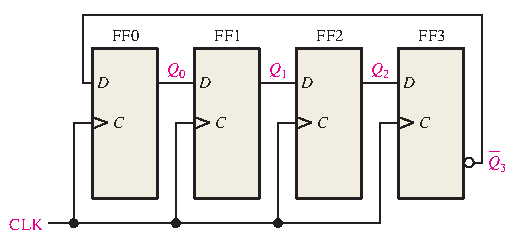
\includegraphics[scale = 0.8]{Graphics/VHDL/Practice 5/COUNTERS/Johnson_Counter_467.pdf}
    \caption{4-bit Johnson counter ~\autocite{FLOYD}}
    \label{fig:JOHNSON_4_BIT}
\end{figure}

\begin{figure}[H]
    \centering
    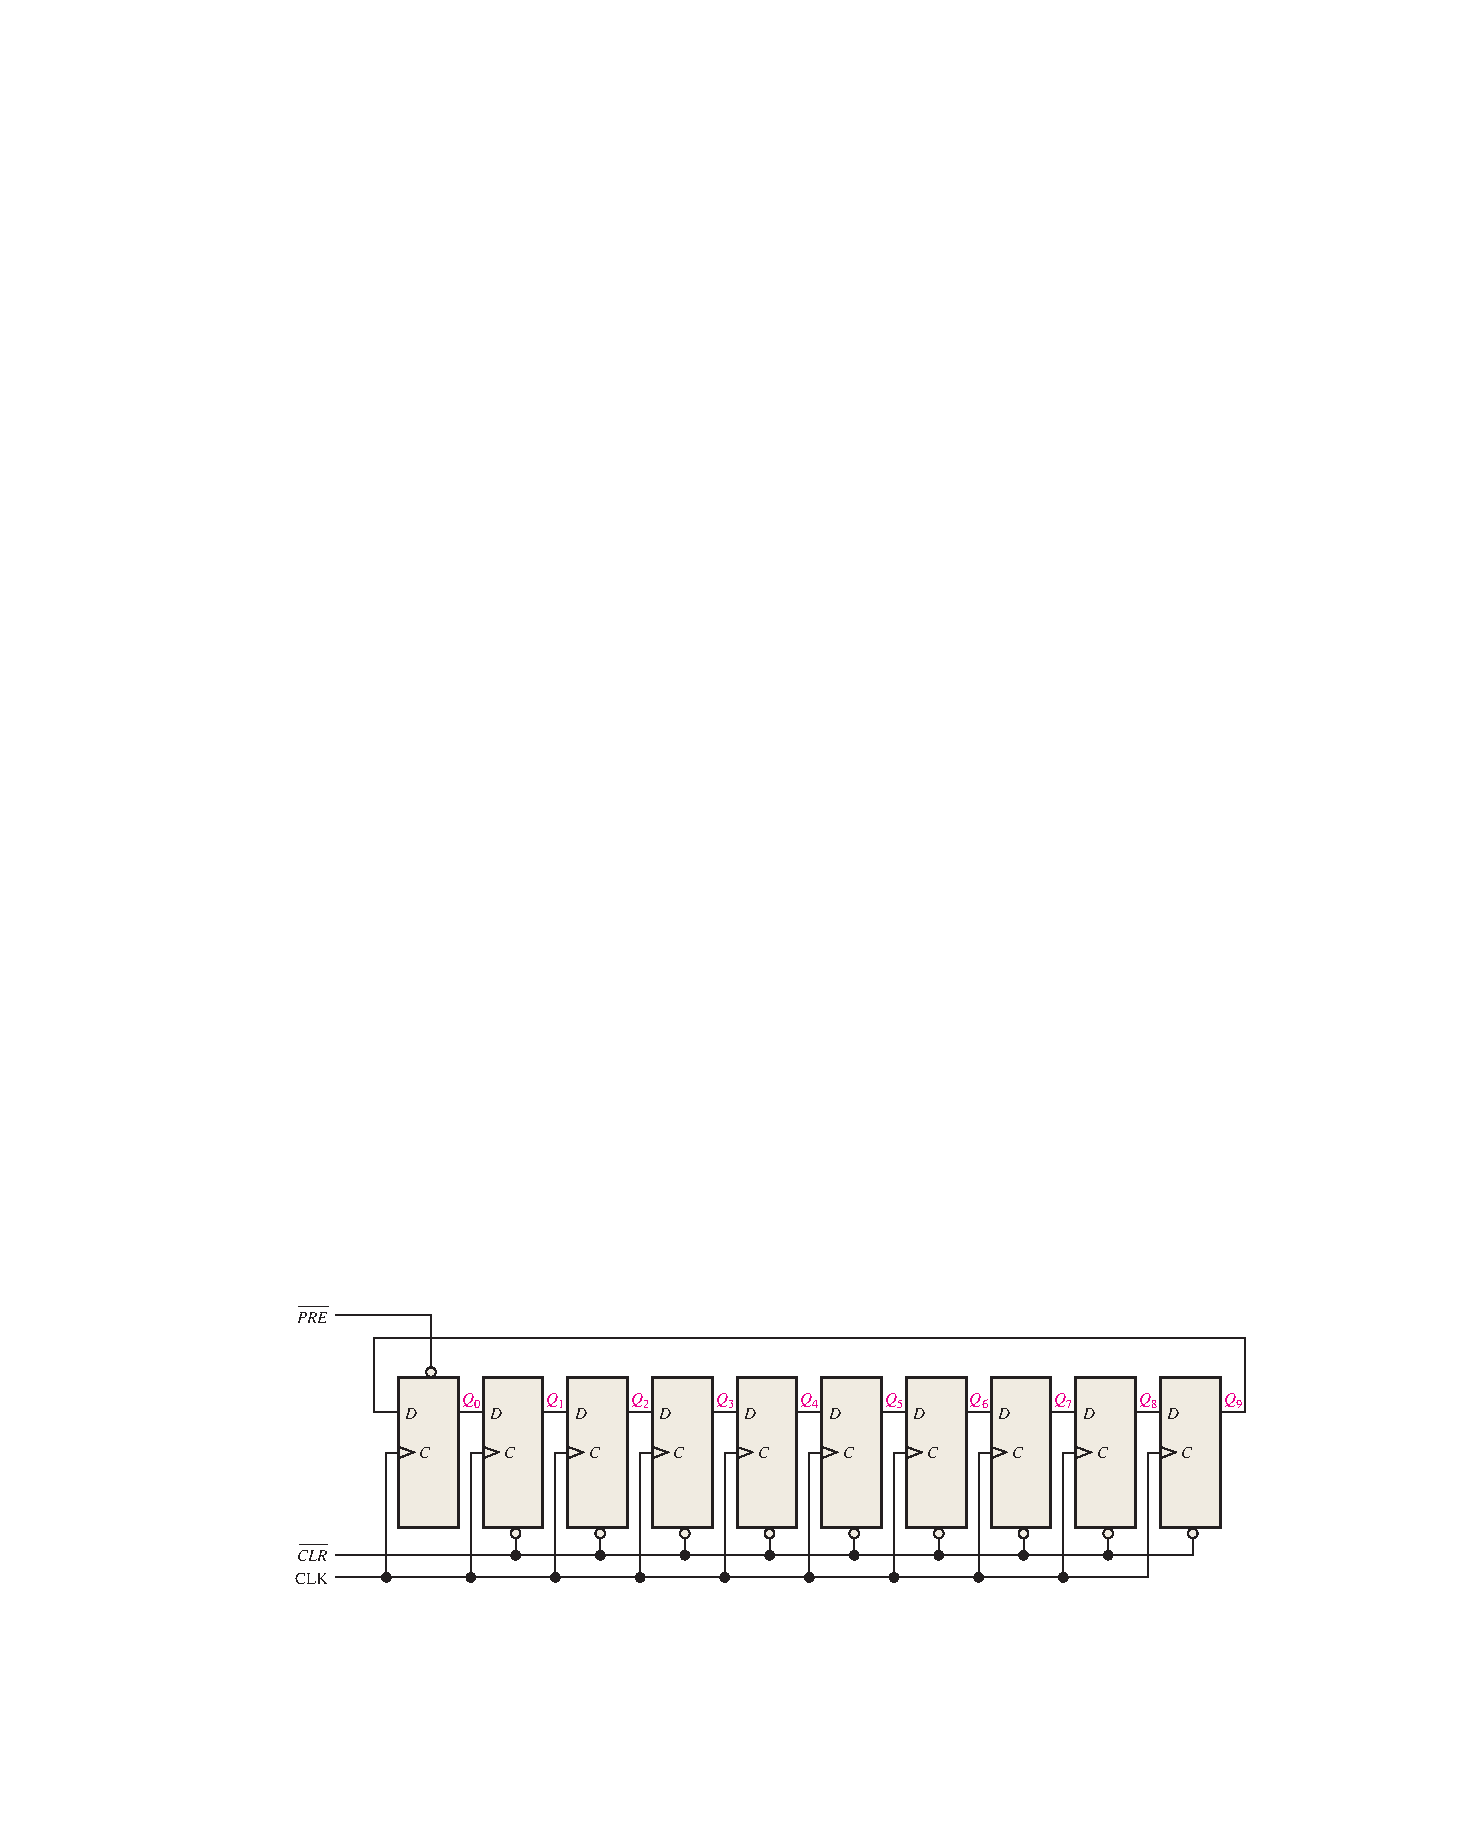
\includegraphics[scale = 0.8]{Graphics/VHDL/Practice 5/COUNTERS/RING_COUNTER.pdf}
    \caption{10-bit Ring counter ~\autocite{FLOYD}}
    \label{fig:RING_10bit}
\end{figure}

\clearpage

\subsubsection{Keypad}
\label{sec:KEYPAD}

In this laboratory practice we have used a 4x3 keypad as a HMI (Human-Machine Interface) so as to allow us to introduce different numbers in our system.\medskip

A keypad is no more than a bi-dimensional array of pushbuttons that are connected together in a matrix configuration in order to reduce the number of data lines that the user must use to read the different signals. We can see this array in the picture attached below:


\begin{figure}[H]
    \centering
    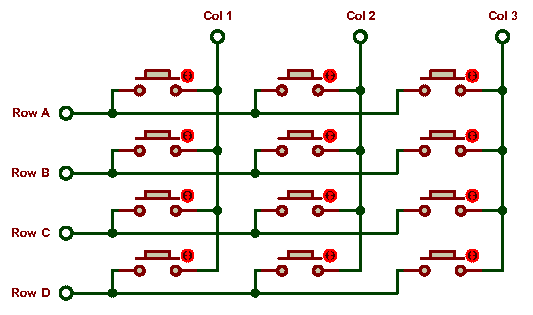
\includegraphics[scale = 1]{Graphics/VHDL/Practice 5/KEYPAD/KEYPAD_BUTTONS.PDF}
    \caption{3x4 Matrix Keypad Pushbutton Array}
    \label{fig:KEYPAD_BUTTON}
\end{figure}

Normally, a ring counter (\textbf{See Subsubsection \ref{sec:COUNTERS} for more on this topic}) is used to circulate a logic \textit{1} in the rows, allowing the CPU to detect which button has been pressed based on the both column in which a HIGH level has been detected and the position of the \textit{1} in the rows. We will dive into this later.\medskip

The proteus representation of this array of buttons can be seen below:\medskip


\begin{figure}[H]
    \centering
    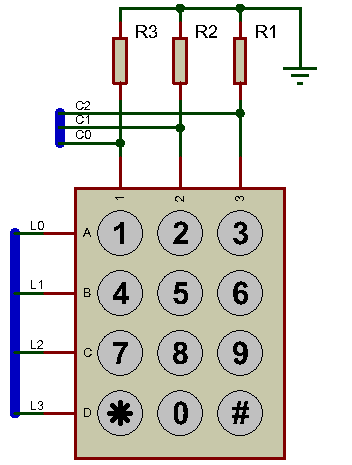
\includegraphics[scale = 0.85]{Graphics/VHDL/Practice 5/KEYPAD/KEYPAD.PDF}
    \caption{Proteus built-in keypad}
    \label{fig:PROTEUS_KEYPAD}
\end{figure}

\clearpage

\subsubsection{7-segment Displays}

A 7-segment display can be described as a module composed of an array of LEDs which are arranged in a special way that enables the user to display different numbers and letters. In this practice we will use them to show the number that the user has entered.\medskip

\begin{figure}[H]
    \centering
    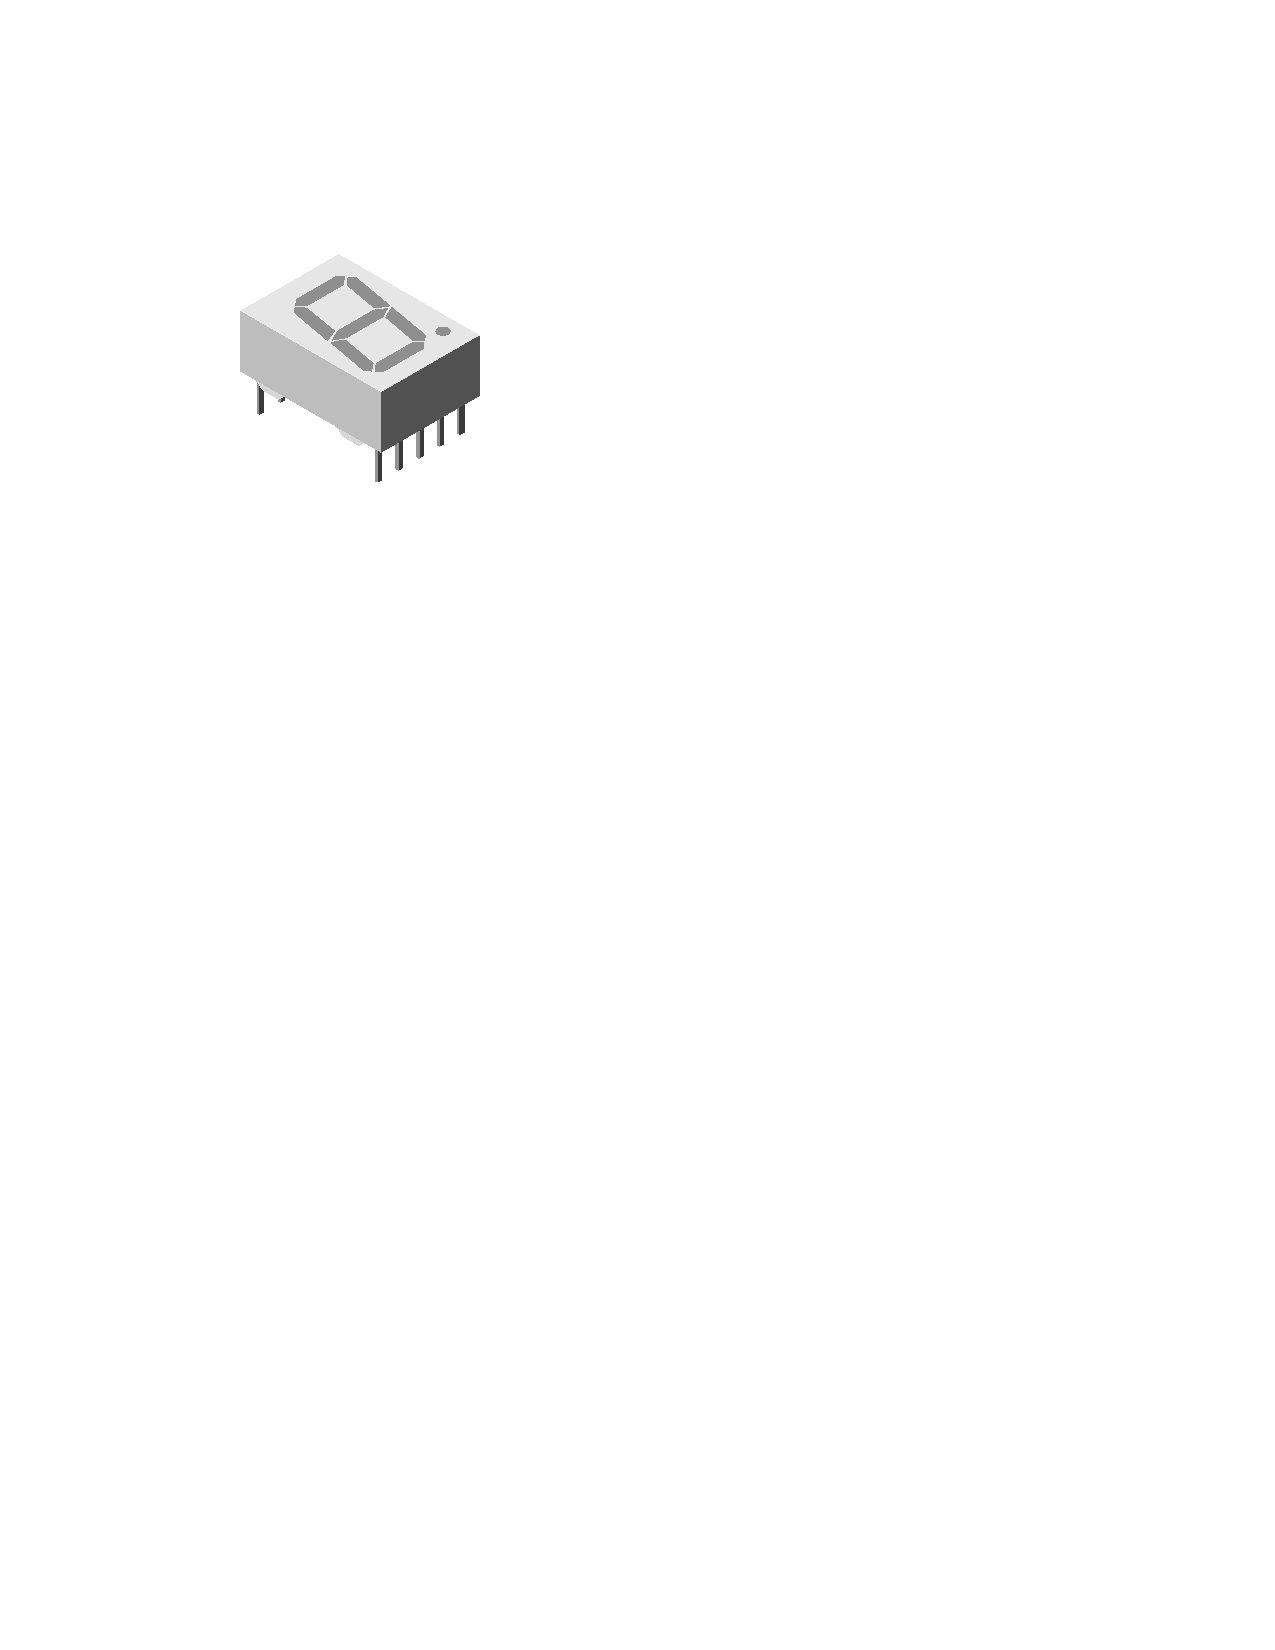
\includegraphics[scale = 0.9]{Graphics/VHDL/Practice 5/7-SEG/3D_MODEL.pdf}
    \caption{3D Model of a 7-Segment display ~\autocite{7-SEGMENT}}
    \label{fig:7-SEG-3D}
\end{figure}

As its name suggests, there are 7 of these LEDs, or segments, plus a decimal point, that may be used to indicate the magnitude of a floating point number. We can see these segments in the following image: \medskip

\begin{figure}[H]
    \centering
    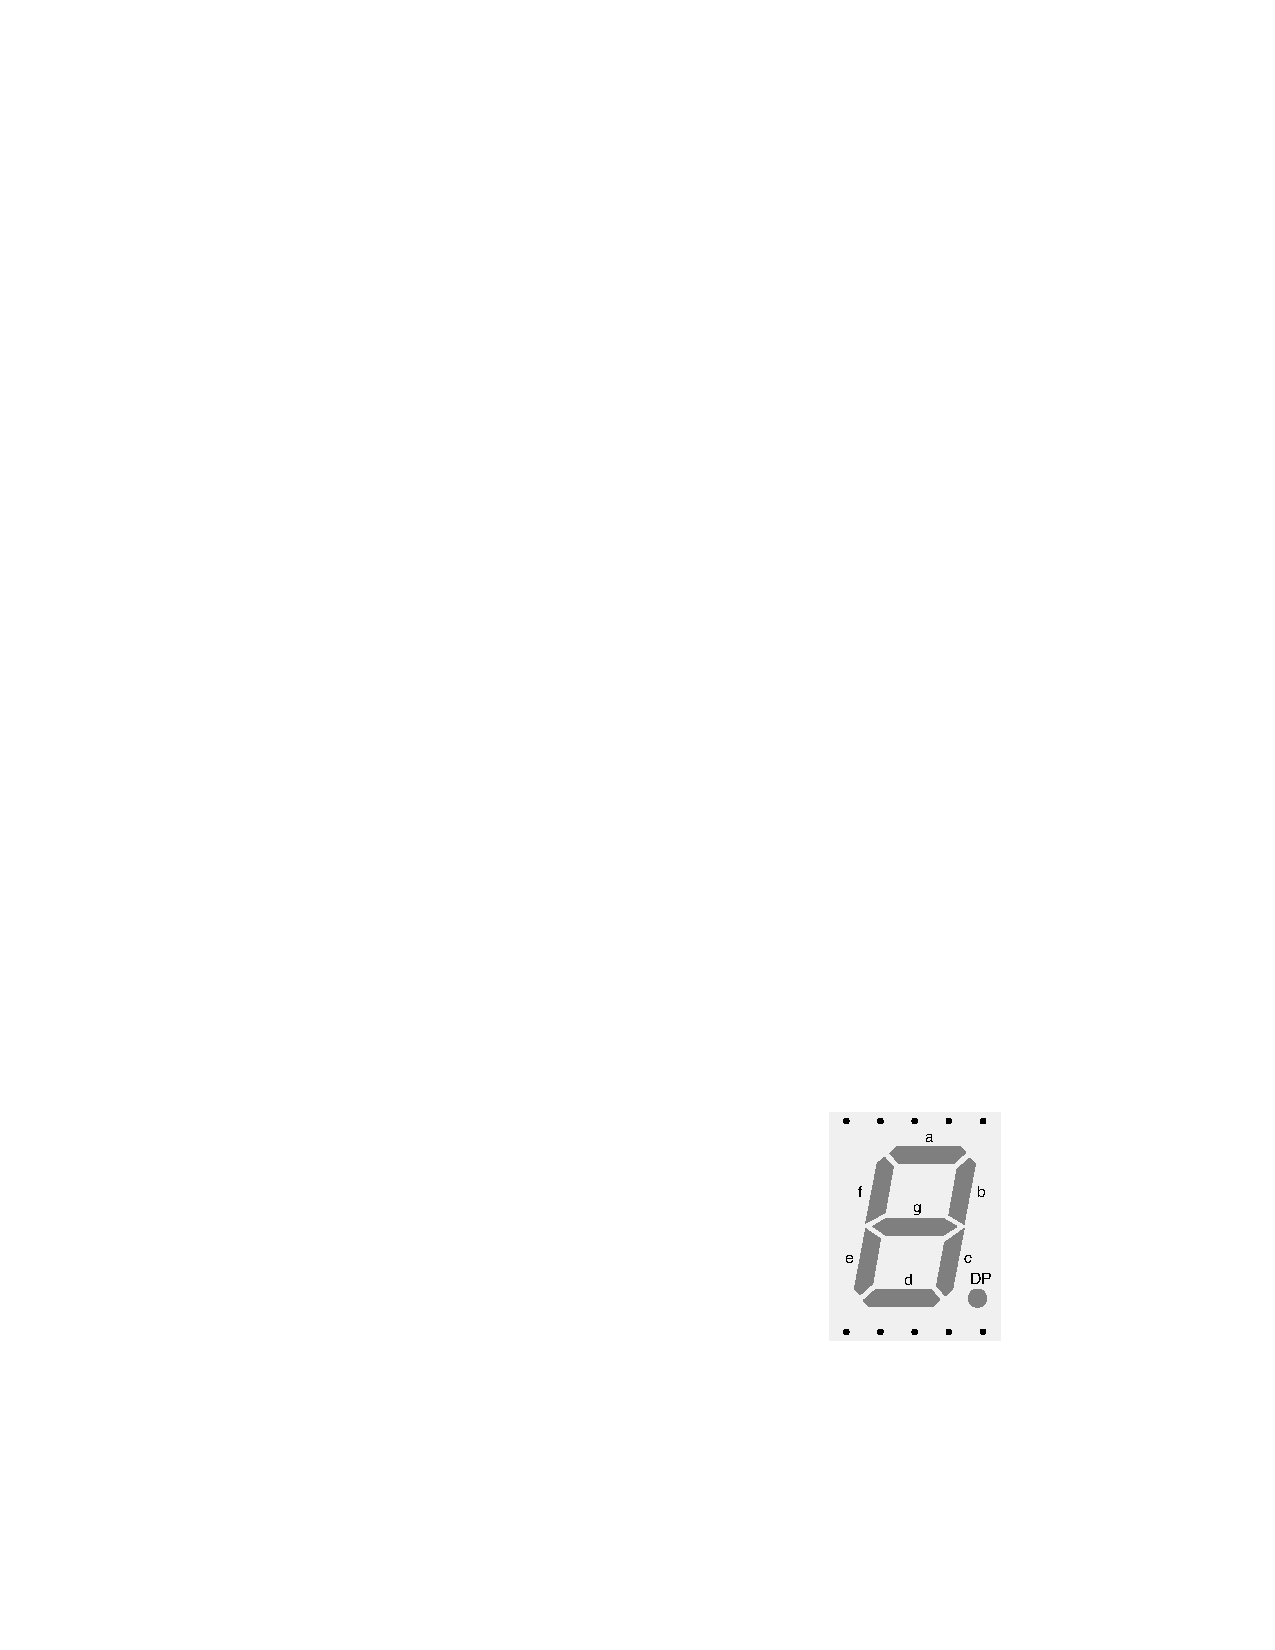
\includegraphics[]{Graphics/VHDL/Practice 5/7-SEG/SEGMENTS.pdf}
    \caption{7-Segment Display individual segments ~\autocite{7-SEGMENT}}
    \label{fig:7-SEG-SEGMENTS}
\end{figure}

\clearpage

Now that we have established how the different elements that make up our circuit work and behave, we will move on to solving the proposed exercises.

\subsection{Exercise 1: Ring Counter with 74HC194}

As we have seen in Subsubsection \ref{sec:COUNTERS}, Ring Counters can be built using Shift Registers, which, in essence, are just multiple Flip-Flops tied together (\textbf{Subsection \ref{sec:FLIP_FLOPS}}). Readily available, off-the-shelf ICs that integrate these kind of counters exist as well. One example of said ICs would be the \textbf{74HC194}. \medskip

\subsubsection{General Description}

The \textbf{74HC194} is a 4-bit bidirectional universal shift register which truth table can be seen below: \medskip

\begin{table}[htbp]
    \resizebox{\columnwidth}{!}{
        \centering
        \begin{tabular}[t]{lccccccccccccc}
            \toprule
            & \textbf{Operating Mode} \vspace{0.2cm} & &\multicolumn{7}{c}{\textbf{Inputs \; \; \; \; \;}} & \multicolumn{4}{c}{\textbf{Outputs}}\\
            
            & & \textbf{CP} & $\mathbf{\overline{MR}}$ & $\mathbf{S_1}$ & $\mathbf{S_0}$ & \textbf{DSR} & \textbf{DSL} & $\mathbf{D_n}$ & & $\mathbf{Q_0}$ & $\mathbf{Q_1}$ & $\mathbf{Q_2}$ & $\mathbf{Q_3}$\\
             
            \midrule
            & \textbf{Reset (clear)} & X & L & X & X & X & X & X & & L & L & L & L\\
            \midrule
            & \textbf{Hold (do nothing)} & X & H & l & l & X & X & X & & q0 & q1 & q2 & q3\\
            \midrule
            & \textbf{Shift Left} & $\uparrow$ & H & h & l & X & l & X & & q1 & q2 & q3 & L\\
            & & $\uparrow$ & H & h & l & X & h & X & & q1 & q2 & q3 & H\\
            \midrule
            & \textbf{Shift Right} & $\uparrow$ & H & l & h & l & X & X & & L & q0 & q1 & q2\\
            & & $\uparrow$ & H & l & h & h & X & X & & H & q0 & q1 & q2\\
            \midrule
            & \textbf{Parallel Load} & $\uparrow$ & H & h & h & X & X & dn & & d0 & d1 & d2 & d3\\
            \bottomrule
        \end{tabular}
        \caption{Functional description of 74HC194 ~\autocite{74HC194}}
        \label{table:74HC194}
        }
\end{table}

The synchronous operation of the device is determined by the mode select inputs ($\mathit{S_0}$, $\mathit{S_1}$). In parallel load mode ($\mathit{S_0}$ and $\mathit{S_1}$ HIGH) data appearing on the $\mathit{D_0}$ to $\mathit{D_3}$ inputs, is transferred to the $\mathit{Q_0}$ to $\mathit{Q_3}$ outputs. When $\mathit{S_0}$ is HIGH and $\mathit{S_1}$ is LOW data is entered serially via \textit{DSL} and shifted from left to right; when $\mathit{S_0}$ is LOW and $\mathit{S_1}$ is HIGH data is entered serially via \textit{DSR} and shifted from right to left. \textit{DSR} and \textit{DSL} allow multistage shift right or shift left data transfers without interfering with parallel load operation. If both $\mathit{S_0}$ and $\mathit{S_1}$ are LOW, existing data is retained in a hold mode. Mode select and data inputs are edge-triggered, responding only to the LOW-to-HIGH transition of the clock (\textit{CP}). Therefore, the only timing restriction is that the mode control and selected data inputs must be stable one set-up time prior to the positive transition of the clock pulse. When LOW, the asynchronous master reset (\textit{MR}) overrides all other input conditions and forces the \textit{Q} outputs LOW. ~\autocite{74HC194}

\clearpage

\subsubsection{Application: Ring Counter}

The aim of the first part of the laboratory lecture is to build a \textbf{ring counter} using a 74HC194. In order to do this, we will follow the following sequence:

\begin{enumerate}
    \item Reset
    \item Parallel Load ($D_n$ = 0100)
    \item Shift Left / Right
\end{enumerate}

This rather simple circuit circuit will allow us to visualize the behaviour of ring counters. We will use ISIS Proteus to perform the simulation:

\begin{figure}[H]
    \centering
 
    \ifnum\value{ANIMATION}=1 {
        \animategraphics[controls,loop,scale=1.1]{1}{Graphics/VHDL/Practice 5/74HC194/ORIGINAL/F}{0}{5}
    } 
    \else {
        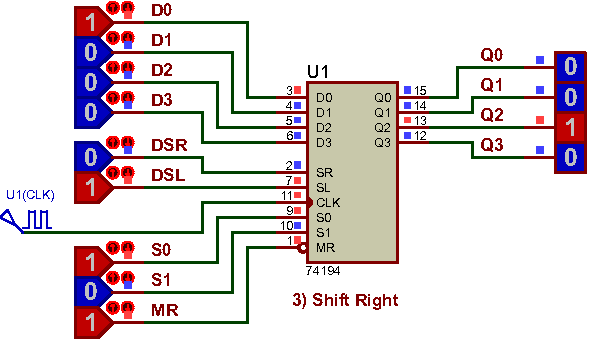
\includegraphics[scale=1.1]{Graphics/VHDL/Practice 5/74HC194/ORIGINAL/F4.PDF}
    }\fi
    
    \caption{Basic Shift Right Operation}
    \label{fig:74HC194_SHIFT_RIGHT}
\end{figure}

As we have seen, the 74HC194 is not a counter but a shift register, which means that once we preload the \textit{1} and we let it run, after just 4 clock cycles, the outputs $Q_n$ will return to \textit{0000}. In other words, the \textit{1} will be shifted right 4 times, and its previous position will be replaced by a \textit{0}, effectively resetting the register.\medskip

To solve this issue, we will connect $Q_3$ back to the \textit{DSR} pin so that when the \textit{1} gets to the last position, the counter preloads itself with \textit{1000} and starts again.\medskip

To control the counter, we will make use of the two selection pins $S_0$ and $S_1$. As we can see in Table \ref{table:74HC194}, when $S_0 = 1$ and $S_1 = 1$, the inputs $D_n$ will be loaded in the output $Q$, and when $S_0 = 1$ and $S_1 = 0$, provided that $DSR = 0$, the counter will start right-shifting the preloaded \textit{1} bit. Once the \textit{1} gets to $Q_3$, the $DSR$ pin will be pulled HIGH and, in the next cycle, the counter will introduce a \textit{1} in $Q_0$ instead of a \textit{0}. This keeps the counter going until the S pins are pulled HIGH, in which case the operation would be halted and the counter would be restarted back to the original state.\medskip

We can see this in the following animation:

\begin{figure}[H]
    \centering
 
    \ifnum\value{ANIMATION}=1 {
        \animategraphics[controls,loop,scale=1.1]{1}{Graphics/VHDL/Practice 5/74HC194/MODIFIED/F}{0}{9}
    } 
    \else {
        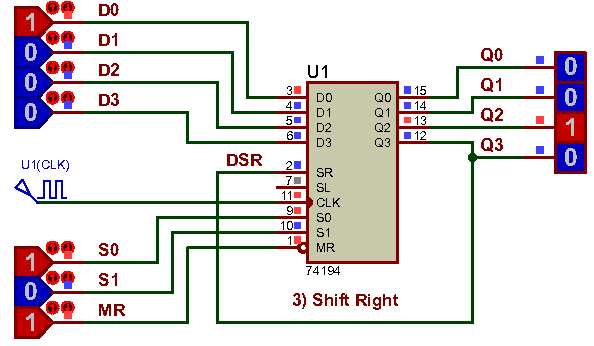
\includegraphics[scale=1.1]{Graphics/VHDL/Practice 5/74HC194/MODIFIED/F4.PDF}
    }\fi
    
    \caption{Ring Counter with 74HC194}
    \label{fig:74HC194_RING}
\end{figure}

\clearpage 

\subsection{Exercise 2: Ring Counter with VHDL}
\label{sec:RING_VHDL}

In this exercise we are asked to implement a ring counter such as the one seen in the previous exercise, but this time using VHDL and a GAL.\medskip

This GAL will include the following I/O:

\begin{itemize}
    \item \textbf{IR} as the synchronous control INPUT.
    \item \textbf{CLK} as the clock INPUT.
    \item $\mathbf{L\left[ 3...0 \right]}$ as the 4 OUTPUTS ($\mathbf{Q_n}$). 
\end{itemize}

The control input, \textit{IR} will operate as folows:

\begin{enumerate}
    \item If a HIGH is detected in this pin, \textit{0001} will be preloaded in the counter.
    \item Once the pin in pulled LOW, the ring counter will be started and it will continue until IR is pulled HIGH again. 
\end{enumerate}

To illustrate this behaviour, a flow diagram has been attached below:

\begin{figure}[H]
    \centering
    \includegraphics[scale = 0.7]{Graphics/VHDL/Practice 5/AXGLYPH/Block_Diagram.pdf}
    \caption{VHDL Ring Counter Flow Diagram}
    \label{fig:VHDL_RING_FLOW}
\end{figure}

\clearpage

The VHDL code that describes this process can be seen below:

\inputcode{CODES/VHDL/Practice_5/RING_COUNTER.vhd}

As we can see, a signal \textit{l\_temp} has been created so as to avoid modifying the outputs directly, as this may cause unwanted results.

\clearpage

\subsection{Exercise 3: 3x4 Keypad Control with VHDL}

This exercise sums up all of the knowledge that we have aquired about different components such as shift registers, counters, 7-segment displays, and so on. \medskip

The aim of this last part is to create a system that displays what the user introduces via a keypad in a 7-segment display. To do this, we will make use of the VHDL ring counter that we have just seen in Subsection \ref{sec:RING_VHDL} to interface the keyboard and we will write what we read back to a BCD to 7-segment dislay driver, which, as the name suggests, will convert the output of the GAL, in BCD, to a readable decimal form in the 7-segment display.\medskip

To interface the keyboard we must use a ring counter so as to reduce the amount of needed pins. Otherwise, the GAL would most probably not be able to read all of the required inputs. For this particular case, a ring counter is used to circulate a logic 1 in the display's rows, allowing the GAL to detect which button has been pressed based on the both column in which a HIGH level has been detected and the position of the 1 in the rows, as seen in \textbf{Subsubsection \ref{sec:KEYPAD}}.\medskip

This GAL will include the following \textbf{inputs}:

\begin{itemize}
    \item \textbf{IR} as the synchronous control.
    \item \textbf{CLK} as the clock.
    \item $\mathbf{C\left[ 2...0 \right]}$ as the logic levels from Keypad columns. They are pulled LOW by default due to the pull-down.
\end{itemize}

Regarding the \textbf{outputs}, we find:

\begin{itemize}
    \item $\mathbf{L\left[ 3...0 \right]}$ as the ring counter outputs. 
    \item $\mathbf{Q\left[ 3...0 \right]}$ as the BCD Code corresponding to the pushed button, as shown the truth table below. 
\end{itemize}


\begin{table}[H]
    \centering
        \begin{tabular}[t]{lcccc}
            \toprule
            &\textbf{L3..L0}&\textbf{C2...C0}&\textbf{Button}&\textbf{BCD code}\\
            \midrule
                &    0001   & 001     & 1      & 0001     \\
                &    0010   & 001     & 4      & 0100     \\
                &    0100   & 001     & 7      & 0111     \\
                &    1000   & 001     & *      & 1100     \\
                &    0001   & 010     & 2      & 0010     \\
                &    0010   & 010     & 5      & 0101     \\
                &    0100   & 010     & 8      & 1000     \\
                &    1000   & 010     & 0      & 0000     \\
                &    0001   & 100     & 3      & 0011     \\
                &    0010   & 100     & 6      & 0110     \\
                &    0100   & 100     & 9      & 1001     \\
                &    1000   & 100     & \#     & 1111     \\
            \bottomrule
        \end{tabular}
        \caption{Reading to Button Conversion table ~\autocite{SLIDES_5}}
        \label{table: KEYPAD_TABLE}
\end{table}


The VHDL code that describes this process can be seen below:

\inputcode{CODES/VHDL/Practice_5/KEYPAD.vhd}

As we explained in Exercise 2 (\textbf{Section \ref{sec:RING_VHDL}}) this code is composed of a ring counter, which is initialized by the \textit{IR} pin, and the rest of the logic. We will not delve into the ring counter part again as it has already been explained before. \medskip

\clearpage

The rest of the code reads the button presses, interprets them and outputs the corresponding BCD code. To do this, we first start the ring counter, which is connected to the L terminals of the keypad. At the same time, we monitor the C lines of said keypad using the output \textit{pulse}. If pulse is pulled HIGH, meaning that one of the buttons has been pressed, we check both the pin of the C array in which the HIGH has been detected as well as the position of the one in the ring counter. Since there can only be one possible combination, i.e., only one row and one column can be active at the same time, the pressed button can be read using this method.\medskip

Once the pressed button has been determined, the GAL outputs its corresponding BCD code in $Q_n$. This output is connected through a BCD to 7-segment converter to the display. \medskip

We can see this here:

\begin{figure}[H]
    \centering
 
    \ifnum\value{ANIMATION}=1 {
        \animategraphics[controls,loop,scale=0.8]{1}{Graphics/VHDL/Practice 5/7-SEG/ANIMATION/F}{0}{9}
    } 
    \else {
        \includegraphics[scale=0.8]{Graphics/VHDL/Practice 5/7-SEG/ANIMATION/F2.PDF}
    }\fi
    
    \caption{Proteus assembly of 3x4 Keypad Control}
    \label{fig:KEYPAD_PROTEUS}
\end{figure}

\clearpage






















\section{Laboratory Lecture 6: Safecode}

The aim of this laboratory lecture is to build a system which stores a 4 digit code, which will be entered by the user using a keypad, as we saw in Practice 5 (\textbf{See Section \ref{sec:KEYPAD_GENERAL} for more on this topic}).\medskip

To achieve this, we will use a reprogrammable temporary storage device, i.e. a RAM, which stands for Random Access Memory. Before diving into the laboratory lecture, we will briefly go over the basics of these type of storage devices.


\subsection{Introduction: Random Access Memory}

The auxiliary memory of a system has the duty of keeping essential information that the Central Processing Unit (CPU), in our case a GAL, needs in order to operate correctly.\medskip

This information is usually kept in words of two bytes (16 bits in total), treated as individual entities or memory locations.\medskip

In order to increment the amount of data that can be stored, memory devices usually combine multiple memory locations into two dimensional arrays (i.e. 8x8 array), or even three dimensional arrays (i.e. 8x8x8 array). We can see this here:\medskip

\begin{figure}[H]
    \centering
    \includegraphics[scale = 0.85]{Graphics/VHDL/Practice 6/RAM/RAM_BLOCK_DIAG.pdf}
    \caption{RAM block diagram ~\autocite{FLOYD}}
    \label{fig:RAM_BLOCK_DIAG}
\end{figure}


\begin{figure}[H]
    \centering
    \includegraphics[scale = 0.85]{Graphics/VHDL/Practice 6/RAM/RAM_BLOCK_CONFIG.pdf}
    \caption{RAM array configuration ~\autocite{FLOYD}}
    \label{fig:RAM_BLOCK_CONFIG}
\end{figure}


\subsubsection{Chip description}

Due to its internal structure, most readily available RAMs use the same pinout. In this practice in particular, we have used a 6116, a 16K (2K x 8-bit) Random Access Memory.\medskip

One example of said pinout can be seen below:

\begin{figure}[H]
    \centering
    \includegraphics[scale = 0.8]{Graphics/VHDL/Practice 6/RAM/RAM_IO.pdf}
    \caption{6116 RAM Pinout ~\autocite{6116}}
    \label{fig:<label>}
\end{figure}

\clearpage

In the graph, we can clearly distinguish 3 main blocks apart from the storage ones, namely the Address bus, the I/O bus and the Control circuitry.\medskip

The different functions of these blocks are described below:

\paragraph{Control circuitry}

The control of most RAMs is performed by changing the state of 3 pins, namely $\overline{CE}$, $\overline{OE}$, and $\overline{WE}$.\medskip

We will now see what the function of these pins is:\medskip


\textbf{Chip Enable} \medskip

To operate the memory first we have to activate the Chip Enable $\overline{CE}$ terminal (Active Low). \medskip

When a CPU has to handle multiple memory chips, in order to read or write from one of them, the other ones are disabled by sending a HIGH to their respective $\overline{CE}$ terminals. \medskip

\textbf{Write Enable} \medskip

With this terminal the CPU specifies if the operation it wants to execute is to write into the memory (LOW at $\overline{WE}$) or to read from it (HIGH at $\overline{WE}$).\medskip


\textbf{Output enable} \medskip

The $\overline{OE}$ connects the output of the memory to the data bus. If it is in LOW, data can be sent from the memory. Otherwise, a HIGH level will create a High-Z output at the Data Bus.  We usually keep it in a constant LOW in order to simplify the system.\medskip

We can see all of the possible operation modes in the table attached below: 

\begin{table}[H]
    \centering
        \begin{tabular}[t]{lccccc}
            \toprule
            & \textbf{Mode} & $\mathbf{\overline{CS}}$ & $\mathbf{\overline{OE}}$ & $\mathbf{\overline{WE}}$ & \textbf{I/O}\\
            \midrule
                &    Standby   &    H   &   X   &   X   &   High-Z        \\
                &    Read      &    L   &   L   &   H   &   $\text{DATA}_{OUT}$    \\
                &    Read      &    L   &   H   &   H   &   High-Z        \\
                &    Write     &    L   &   X   &   L   &   $\text{DATA}_{IN}$     \\
            \bottomrule
        \end{tabular}
        \caption{Operation Modes Truth Table ~\autocite{6116}}
        \label{table: RAM_MODES}
\end{table}

\clearpage

\paragraph{Address bus}

The Address decoder bus reads the address that the user provides, by pulling the different address pins $\mathbf{\left[ A_0...A_{10} \right]}$ either HIGH or LOW, and it points the memory to that it. In essence, when the user selects an address, depending on the configuration of the control pins, the RAM will either write information to that specific address or read it from it. 


\paragraph{I/O bus}

The I/O bus, as the name suggest is an array of pins that are used to both write information to the RAM or to read from it, depending, again, on the configuration of the Control circuitry. When the RAM is in program mode, i.e. writing mode, the state of these pins will be saved into the address specified by the user. On the other hand, when the RAM is in read mode, the contents of the selected address will appear on this bus.\medskip


In order to simplify the operation, as only 4 digits will be stored, we will only use the $A_0$ and $A_1$ Address terminals. Besides, as we only need to store digits from 0 to 9, only the first 4 bits of the I/O Bus will be used.\medskip

We can see the different pins that we have just discussed in the following image:\medskip

\begin{figure}[H]
    \centering
    \includegraphics[scale = 1.2]{Graphics/VHDL/Practice 6/RAM/RAM_PROTEUS.PDF}
    \caption{Proteus Subassembly of RAM}
    \label{fig:RAM_PROTEUS_Subassembly}
\end{figure}

\clearpage

\subsection{Exercise 1: Safecode}

Now that we have seen how RAM ICs work, we will move on to the practice itself. As we said before, the aim of this practice is to design and build a system that takes a number, entered by the user using a keypad, and stores it into the RAM for later use. 

\subsubsection{Writing Operation}
\label{sec:WRITING_OPERATION}

In order to be able to both read and store the number, we will use two GALs. One of them will be the one described in the last laboratory lecture (\textbf{See Section \ref{sec:KEYPAD_GENERAL} for more on this topic}) and the other corresponds to the one desgined in this lecture. 

The inputs of this GAL will be:

\begin{itemize}
    \item \textbf{CLK:} Clock input.
    \item \textbf{SIG:} The BCD code coming from the first GAL.
\end{itemize}

On the other hand, the outputs will be:

\begin{itemize}
    \item \textbf{D:} Password output (To program the RAM).
    \item \textbf{CS:} Chip select (To select between Write and Standby Mode)
    \item \textbf{A:} Address (As INOUT) to select the address to which the GAL must write.
\end{itemize}

We can see this in the following image:

\begin{figure}[H]
    \centering
    \includegraphics[scale = 1.15]{Graphics/VHDL/Practice 6/SAFECODE/SAFECODE_PROTEUS_GAL.PDF}
    \caption{Proteus Subassembly of Safecode}
    \label{fig:SAFECODE_PROTEUS}
\end{figure}

\clearpage

The memory device will start storing data when the Write Enable ($\overline{WE}$) signal and the Chip Select ($\overline{CS}$) are pulled LOW by the GAL. A timing diagram is attached:\medskip


\begin{figure}[H]
    \centering
    \includegraphics[scale = 0.60]{Graphics/VHDL/Practice 6/RAM/6116.pdf}
    \caption{6116 RAM Write Cycle ~\autocite{6116}}
    \label{fig:6116}
\end{figure}


The general truth table of this specific RAM, though it is mostly the same for most RAM chips, can be found in \textbf{Table} \textbf{\ref{table: RAM_MODES}} \medskip

Now we will discuss the different states that we have defined in our FSM. As per before, the full code will be attached as well.

\subsubsection{FSM States Overview}

\hspace{0.4cm}
    \bm{$Q_0$}
\medskip

At rest, the system must start at Address "00", and the $\overline{CS}$ signal must be pulled HIGH do to it being active LOW. Once the $*$ button is pressed, system transitions to $Q_1$ state.

\medskip
    \bm{$Q_1$}
\medskip

The $\overline{CS}$ signal is pulled LOW level, and the RAM device is in the “ready to write” state $Q_1$. This means that from now on, Address number $00$ is ready to be overwritten by the character we introduce with the keypad. \medskip

When introducing a new character with the keypad, pressing $*$ repeatedly will make the system stay in $Q_1$, pressing the \textit{\#} character will make the system return to $Q_0$, and pressing any other character will make the system change to State $Q_2$. \medskip

\bm{$Q_2$} \textbf{\&} \bm{$Q_3 \textit{\textbf{ and return to }} Q_0$}\medskip

In state $Q_2$, the character previously introduced is written on the address $00$.\medskip

\clearpage

Now, there are two options, either to keep writing to the memory, or to stop writing:

\begin{itemize}
    \item In order to keep writing, any key pressed but \textit{\#} and the \textbf{same key} \footnote{The password cannot contain consecutive digits due to the memory limitations of the GAL. For instance \textit{1212} would be a valid password, but \textit{1122} would not.}, will transition the system to state $Q_3$, where the system jumps to the next Address (where the next character will be kept), and the writing loop starts again at \textit{$Q_1$}.
    
    \item In order to stop, the  \textit{\#} button is pressed, and the system returns to state \textit{$Q_0$}, meaning that  the Address is reset to $00$, and the writing operation ends.
\end{itemize}


To illustrate the different states and the transitions between them we have included the following diagram:\medskip

\begin{figure}[H]
    \centering
    \includegraphics[scale = 0.55]{Graphics/VHDL/Practice 6/SAFECODE/SAFECODE_FSM.pdf}
    \caption{Safecode FSM}
    \label{fig:SAFECODE_FSM}
\end{figure}

\clearpage

The VHDL code for this GAL can be found below:

\inputcode{CODES/VHDL/Practice_6/SAFECODE.vhd}

The final Proteus assembly can be found below:

\begin{figure}[H]
    \centering
 
    \ifnum\value{ANIMATION}=1 {
        \animategraphics[controls,loop,scale=0.78]{1}{Graphics/VHDL/Practice 6/SAFECODE/ANIMATION/F}{0}{5}
    } 
    \else {
        \includegraphics[scale=0.78]{Graphics/VHDL/Practice 6/SAFECODE/ANIMATION/F2.pdf}
    }\fi
    
    \caption{Proteus Assembly of Safecode}
    \label{fig:PROTEUS_SAFECODE_ASSEMBLY_FINAL}
\end{figure}
            
After introducing the code, we can pause the simulation and check that indeed, the "Memory Contents" pop-up window displays the entered data.\medskip

\begin{table}[H]
    \centering
        \begin{tabular}[t]{lccccc}
            \toprule
                &\multicolumn{5}{c}{\textbf{Memory Contents}}\\
                & 0000 & 01 & 02 & 03 & 04 \\
            \bottomrule
        \end{tabular}
        \caption{RAM Contents}
        \label{table:RAM_CONTENTS}
\end{table}

\clearpage

















\section{Laboratory Lecture 8: Integrated Circuit Technologies}

\subsection{Introduction}

The main objective of this practice is to get a grasp of the most important characteristics of logic families and their usage in real-life circuits.\medskip

As we have discussed in previous practices, logic gates are a staple in the field of digital electronics. Something that we have not discussed until know is the concept of \textbf{\textit{logic families}}. \medskip

During the production of digital integrated circuits, different circuit configurations and production technologies are used. Each of these approaches can be refered to as a specific \textbf{logic family}. The idea behind having different approaches, or different logic families, is that each IC of same family will have identical electrical characteristics, and because of that, will be compatible with each other. These characteristics, which are bound to be identical, are, for instace, supply voltage range, speed of response, power dissipation, input and output logic levels, current sinking and sourcing capability, noise margin, fan-out, to name a few.\medskip

Nowadays, there are 2 important logic families that comprise most of the ICs that one may find, namely \textbf{\textit{Bipolar families}} and \textbf{\textit{MOS (Metal oxide semiconductor) families}}. The first family is formed by technologies such as diode logic (DL), emitted coupled logic (ECL), resistor transistor logic (RTL), diode transistor logic (DTL), transistor transistor logic (TTL), whereas the latter is composed of PMOS, NMOS, CMOS. There is also a special type of logic family that combines both bipolar and CMOS, called Bi-CMOS. \medskip

Out of the above mentioned families DL, RTL and DTL are not used these days, as they have become obsolete. TTL, CMOS, ECL, NMOS and Bi-CMOS, on the other hand, continue to be used in electronic devices nowadays.\medskip

In general, CMOS devices have greater noise immunity and draw less power, due to the way in which the internal switching is performed, i.e. by applying a specific voltage to the gate of the FET, as opposed to TTL devices, which require polarizing currents to operate. Besides, due to the insignificant power draw, the CMOS family dissipates less energy as heat. \medskip

The term \textbf{\textit{noise inmunity}} refers to the circuit's ability to tolerate noise, i.e.unwanted voltages which are normally induced in logic circuits by electric/magnetic fields, without changes. As we have said, the noise inmunity of CMOS devices is greater than the one of TTL devices. We can see this in the following image. \medskip


\begin{figure}[H]
    \centering
    \includegraphics[scale = 0.8]{Graphics/VHDL/Practice 8/TTL_VS_CMOS.pdf}
    \caption{TTL vs CMOS noise margins~\autocite{LOGIC_GUIDE}}
    \label{fig:TTL_VS_CMOS}
\end{figure}

In this image we can see the different voltage levels that define each family. A brief definition of each one can be found below:

\begin{itemize}
    \item $\mathbf{V_{OH (MIN)} - \text{High-Level Input Voltage}}$: The minimum voltage level require for a logic 1 at the \textit{input}. Any voltage below this level will not be accepted as a HIGH by the logical circuit. 

    \item $\mathbf{V_{IL (MAX)} - \text{Low-Level Input Voltage}}$: The maximum voltage level require for a logic 0 at the \textit{input}. Any voltage above this level will not be accepted as a LOW by the logical circuit. 

    \item $\mathbf{V_{OH (MIN)} - \text{High-Level Output Voltage}}$: The minimum \textit{output} voltage for a logic 1 under defined load conditions.

    \item $\mathbf{V_{OL (MAX)} - \text{Low-Level Output Voltage}}$: The maximum \textit{output} voltage for a logic 0 under defined load conditions.
\end{itemize}

For proper operation, logic circuit input voltage levels must be kept out of the indeterminate range, i.e. lower than $\mathbf{V_{IL (MAX)}}$ or higher than $\mathbf{V_{IH (MIN)}}$.\medskip

To calculate the noise inmunity, we have to calculate both the High-state noise margin and the Low-state one. The difference between the tolerable output and input ranges is called the noise margin of the gate. 

\begin{align*}
    V_{NH} &= V_{OH (MIN)} - V_{OH (MIN)} \\
    V_{NL} &= V_{IL (MAX)} - V_{OL (MAX)}
\end{align*}\medskip


Before diving into the practice itself, we will briefly go over the main components that will be used in this practice.

\subsubsection{Inverter Logic Gate: 74HCT04}

74HCT04 is nothing more than an array of 6 CMOS inverter logic gates with standard push-pull outputs. \medskip

From the datasheet~\autocite{74HCT04}, we can obtain the values of the parameters that we described ealier. 

\begin{table}[ht]
    \centering
        \begin{tabular}[t]{lcccc}
            \toprule
            & \textbf{Symbol} & \textbf{Parameter} & \textbf{Min} & \textbf{Max} \\
            \midrule
            & $V_{IH}$ & High-Level Input Voltage  & 2.0         &             \\
            & $V_{IL}$ & Low-Level Input Voltage   & \textendash & 0.8         \\
            & $V_{OH}$ & High-Level Output Voltage & 4.4         & \textendash \\
            & $V_{OL}$ & Low-Level Output Voltage  & 3.8         & \textendash \\
            \bottomrule
        \end{tabular}
        \caption{74HCT04 CMOS Voltage Levels}
        \label{table:74HCT04_VOLT_LEVELS}
\end{table}

These values will be used later on in the practice.

\subsubsection{BJT: BD315}

Transistors, in general, are 3 terminal active devices made from different semiconductor materials such as silicon or germanium that can act as either an insulator, or a conductor, depending on the electrical signal that is supplied to them. The transistor’s ability to change between these two states enables it to have two basic functions: \textbf{\textit{switching}} (digital electronics) or \textbf{\textit{amplification}} (analogue electronics)\medskip

There are 2 major types of transistors, namely \textbf{BJTs} and \textbf{FETs}. BJT stands for \textbf{Bipolar Junction Transistor} whereas FET stands for \textbf{Field-Effect Transistor}. The first type of transistors are controlled by sourcing or sinking current to their base terminal (NPN or PNP, respectively), unlike the latter, which are controlled by applying a voltage, to their gate terminal (NMOS or PMOS). \medskip

Transistors are one of the most important components in electronics, as they are used in almost every active component. Logic gates, for instance, use transistors to perform the internal switching operations. As saw in the last section, TTL devices use BJTs, and CMOS use FETs.\medskip

The \textbf{BD135} can be described as an NPN BJT. As we have said, BJTs are controlled by current. In the case of NPNs, a small current has to be supplied to their base terminal for them to work. PNPs, on the other hand need to have some current sinked out of their base terminal for them to work properly.\medskip

\clearpage

Depending on the amount of current that one sinks/sources, to/from their base terminal, they will operate in different regions, namely:

\begin{itemize}
    \item \textbf{Active Region:} The transistor behaves as an amplifier. 
    \item \textbf{Saturation:} The transistor behaves as a switch.
    \item \textbf{Cut-off:} The transistor is OFF $\rightarrow$ No current flow.
\end{itemize}

This 3 operation modes can be seen in the following image:

\begin{figure}[H]
    \centering
    \includegraphics[width = \textwidth]{Graphics/VHDL/Practice 8/BJT/IC_VCE.pdf}
    \caption{BJT (NPN) operation modes~\autocite{BOYLESTAD}}
    \label{fig:BJT_MODES}
\end{figure}


As it can be seen in the graph, the active region represents a zone in which the colector current is proportional to the base current. This relationship can be expressed by the following equation:

\begin{equation*}
    I_C = \beta \cdot I_B
\end{equation*}

\noindent Where $\beta$ is the gain, a value that can be considered constant for each transistor and $I_C$ and $I_B$ are the collector and base currents respectively. \medskip

An example circuit can be seen below:

\begin{figure}[H]
    \centering
    \includegraphics[scale = 1]{Graphics/VHDL/Practice 8/BJT/NPN_CIRCUIT.pdf}
    \caption{NPN example circuit~\autocite{BOYLESTAD}}
    \label{fig:NPN_EXAMPLE}
\end{figure}

The $V_{CE}$, or the Collector-to-Emitter voltage, is also plotted in the image. As the current that passes through the load, $I_C$, increases, the $V_{CE}$ decreases, that is, the more power that the load dissipates, the less power that the BJT has to dissipate. There is a point in which the equation described above does not hold anymore. This critical point is reached when the $I_C$ is maximum, and so the $V_{CE}$ is minimum. If more base current were to be sourced to the base of the NPN, the $I_C$ would NOT increase linearly.\medskip

Once this point is reached, the NPN is in Saturation, i.e., it behaves like a switch. In this operation mode, the $V_{CE} \approx 0.1-0.2 \; V$, and the $V_{BE} \approx 0.8 \; V$.

\subsection{Exercise 1: Light Control}

\textit{\textbf{Exercise 1:}} \textit{It is wanted to design a light control by using a LDR (Light Dependent Resistor). The system has to have an input interface circuit in order to adapt the LDR signal. When the LDR works in an absolutely darkness or in a complete brightness, the interface circuit has to work with HCT compatible logic levels.}

\begin{figure}[H]
    \centering
    \includegraphics[scale = 0.9]{Graphics/VHDL/Practice 8/EXERCISE_1/EX_1.PDF}
    \caption{Exercise 1 Assembly}
    \label{fig:EX_1}
\end{figure} \medskip

The ohmic values of the LDR are given:

\begin{itemize}
    \item $R_{LDR} \left( \text{brightness} \right) = 3.5 \; k\Omega$
    \item $R_{LDR} \left( \text{darkness} \right) = 4.8 \; M\Omega$
\end{itemize}

\clearpage

\textbf{a) Calculate the value of} $\mathbf{R_1}$ \textbf{that allows us to fix the 74HCT04 activation values.}\medskip

To calculate the value of $R_1$, we will use the values of $V_{IL}$ and $V_{IH}$ described in Table \ref{table:74HCT04_VOLT_LEVELS} as well as the LDR resistance values given by the exercise.\medskip

\vspace{-0.5cm}

\begin{alignat*}{2}
    V_{IL} &= 0.8 \; V = 5 \cdot \left( \dfrac{R_1}{R_1 + 3.5 \; k\Omega} \right)  &&\rightarrow R_1 = 666.666 \; \Omega \\[7pt]
    V_{IH} &= 2.0 \; V = 5 \cdot \left( \dfrac{R_1}{R_1 + 4.8 \; M\Omega} \right)  &&\rightarrow R_1 = 3.2  \; M\Omega
\end{alignat*}

So we know that $ 666.666 \; \Omega \leq R_1 \leq 3.2 \; M\Omega$ \bigskip

\textbf{b) The system has to control a 12 V, 2 W lamp in such a way that when the LDR detects the darkness the lamp turns on and when the LDR detects the brightness the lamp turns off. The 74HCT04 is not able to do it by itself, why?}\medskip

The 74HCT04 cannot control the lamp by itself because it cannot provide neither enoygh voltage nor enough current. An interface circuit is needed. \bigskip

\textbf{c) Design the necessary interface circuit by using BD135}\medskip

To design the interface circuit of Figure \ref{fig:EX_1}, we will again need the value of $V_{OH}$, which was provided by the datasheet~\autocite{74HCT04} of the 74HCT04, and some of the values that we discussed previously, namely the $I_C$, the $V_{BE(SAT)}$, the $V_{CE(SAT)}$, and the $\beta$.\medskip

The first value, $I_C$ can be obtained from the given specifications, i.e., that the lamp is fed with 12V and it dissipates 2W. An approximation of the collector current can be obtained by just dividing the power by the voltage, that is:

\begin{equation*}
    I_C \approx \frac{2 \; W}{12 \; V} = 166.67 \; mA
\end{equation*}


This value is not exact, as the $V_{CE(SAT)} \neq 0$.\medskip

Assuming the power to be constant, we could say that the real value of $I_C$ is:

\begin{equation*}
    I_C = \frac{2 \; W}{12 \; V - V_{CE(SAT)}}
\end{equation*}

\clearpage

In order to obtain the value of $V_{CE(SAT)}$ as well as the rest of the values we have to resort to the datasheet of the BD135~\autocite{BD135}:

\begin{figure}[H]
    \centering
    \includegraphics[]{Graphics/VHDL/Practice 8/BJT/DATASHEET/VCE-IC.pdf}
    \caption{Collector-Emitter Saturation Voltage~\autocite{BD135}}
    \label{fig:VCE_SAT}
\end{figure}


\begin{figure}[H]
    \centering
    \includegraphics[]{Graphics/VHDL/Practice 8/BJT/DATASHEET/VBE-IC.pdf}
    \caption{Base-Emitter Saturation Voltage~\autocite{BD135}}
    \label{fig:VBE_SAT}
\end{figure}

\begin{figure}[H]
    \centering
    \includegraphics[]{Graphics/VHDL/Practice 8/BJT/DATASHEET/BETA-IC.pdf}
    \caption{DC Current Gain~\autocite{BD135}}
    \label{fig:DC_GAIN}
\end{figure}

From Figure \ref{fig:VCE_SAT}, we obtain that for a collector current, $I_C \approx 166.67 \; mA$, the $\bm{V_{CE(SAT)} \approx 0.05 \;V}$. Then the \textit{real} value of $I_C$ can be calculated as:

\begin{equation*}
    I_C = \frac{2 \; W}{12 \; V - 0.05} = 167.36 \; mA
\end{equation*}

\noindent From Figure \ref{fig:VBE_SAT} we obtain that, for a $I_C = 167.36 \; mA$ the $\bm{V_{BE(SAT)} \approx 0.8 \; V}$.\medskip

\noindent Finally, from Figure \ref{fig:DC_GAIN} we obtain that, for a $I_C = 167.36 \; mA$, the $\bm{\beta \approx 115}$ \medskip

\noindent With this values, we can calculate the value of $R_B$ following this fashion:

\begin{equation*}
    R_B = \frac{V_{OH} - V_{BE(SAT)}}{\dfrac{I_C}{\beta}} = \frac{4.4 - 0.8}{\left( \dfrac{166.67 \; mA}{115} \right)} = 2484 \; \Omega
\end{equation*}\medskip

Since the obtained value does not belong to the E-12 series, we will choose $\bm{2.2 \; k\Omega}$, as it will guarantee that enough current is sourced.

\clearpage




























\part{Microcontrollers} 
\clearpage

\section{Laboratory Lecture 1: Stepper Motor Controller}

The aim of this laboratory session is to design a stepper motor controller using an ATMega328P microcontroller. Since the basics of stepper motors have already been covered in \textbf{Section \ref{sec:STEPPER_MOTOR}}, they will not be discussed again. However, a brief introduction to the ATMega328p is necessary to fully understand this laboratory session.

\subsection{Introduction}

The Atmel ATMega328P is an 8-bit, low-power CMOS 8-bit microcontroller based on the AVR enhanced RISC architecture. It is built around a Harvard architecture, which means that the Data Memory bus and the Program memory bus are different. In this specific case, it can be said that its data word size is 8 bits and its program word size is 16 bits.\medskip 

The AVR core combines a rich instruction set with 32 general purpose working registers. All the 32 registers are directly connected to the arithmetic logic unit (ALU), allowing two independent registers to be accessed in one single instruction executed in one clock cycle. The resulting architecture is more code efficient while achieving throughputs up to ten times faster than conventional CISC microcontrollers.\medskip

The Atmel ATMega328P provides the following features: 32K bytes of in-system programmable flash with read-while-write capabilities, 1K bytes EEPROM, 2K bytes SRAM, 23 general purpose I/O lines, 32 general purpose working registers, three flexible Timer/Counters with compare modes, internal and external interrupts, a serial programmable USART, a byte oriented 2-wire serial interface, an SPI serial port, a 6-channel 10-bit ADC (8 channels in TQFP and QFN/MLF packages), a programmable watchdog timer with internal oscillator, and five software selectable power saving modes. The idle mode stops the CPU while allowing the SRAM, Timer/Counters, USART, 2-wire serial interface, SPI port, and interrupt system to continue functioning. The power-down mode saves the register contents but freezes the oscillator, disabling all other chip functions until the next interrupt or hardware reset. In power-save mode, the asynchronous timer continues to run, allowing the user to maintain a timer base while the rest of the device is sleeping. The ADC noise reduction mode stops the CPU and all I/O modules except asynchronous timer and ADC, to minimize switching noise during ADC conversions. In standby mode, the crystal/resonator oscillator is running while the rest of the device is sleeping. This allows very fast start-up combined with low power consumption.\medskip

The device is manufactured using Atmel high density non-volatile memory technology. The on-chip ISP flash allows the program memory to be reprogrammed in-system through an SPI serial interface, by a conventional non-volatile memory programmer, or by an on-chip boot program running on the AVR core. The boot program can use any interface to download the application program in the application flash memory. Software in the boot flash section will continue to run while the application flash section is updated, providing true read-while-write operation. By combining an 8-bit RISC CPU within-system self-programmable flash on a monolithic chip, the Atmel ATmega328P is a powerful microcontroller that provides a highly flexible and cost effective solution to many embedded control applications.\medskip

The ATMega328P AVR is supported with a full suite of program and system development tools including: C compilers, macro assemblers, program debugger/simulators, in-circuit emulators, and evaluation kits.~\autocite{ATMEGA328P}\medskip

A diagram describing its pinout can be found below:

\begin{figure}[H]
    \centering
    \includegraphics[scale = 0.55]{Graphics/MICROS/Practice 1/ARDUINO/ATMEGA328P_PINOUT.pdf}
    \caption{ATMega328p's Pinout~\autocite{ATMEGA328P_PINOUT}}
    \label{fig:ATMEGA328P_PINOUT}
\end{figure}


\subsection{Arduino}

The popularity of the ATMega328P can be attributed to its use in the Arduino development board, the design of which falls within the Open Source Hardware category/movement. For our designs, as well as for real-life testing, we will use this board, in particular the Arduino UNO, which breaks out most of the pins into headers, supplies the ATMega with a stable voltage and provides native USB communication.\medskip

A diagram of the Arduino UNO board can be found below:

\begin{figure}[H]
    \centering
    \includegraphics[scale = 0.50]{Graphics/MICROS/Practice 1/ARDUINO/BOARD.pdf}
    \caption{Arduino UNO Pinout~\autocite{BQ_ARDUINO}}
    \label{fig:ARDUINO_UNO_BOARD}
\end{figure}

\subsection{I/O Ports}

The I/O ports allow the user to communicate with the ATMega. All AVR ports, in general, can be said to have have true Read-Modify-Write functionality when used as general digital I/O ports. This means that the direction of one port pin can be changed without unintentionally changing the direction of any other pin.\medskip

The ATMega328P has 3 8-bit ports, namely B, C, D. Each port is controlled by three 8-bit registers:

\begin{enumerate}
    \item \textbf{DDRx -} Direction Register
        \begin{itemize}
            \item Defines wheter a pin in as input (0) or an output (1)
        \end{itemize}
    \item \textbf{PINx -} Pin Input Value
        \begin{itemize}
            \item Reading this register bit returns the value of the specific pin.
        \end{itemize}
    \item \textbf{PORTx - } Pin Output Value:
        \begin{itemize}
            \item Writing to this register SETS the value of a pin.
        \end{itemize}
\end{enumerate}

The internal circuit that controls the state of each pin can be seen below:

\begin{figure}[H]
    \centering
    \includegraphics[scale = 0.9]{Graphics/MICROS/Practice 1/ARDUINO/INTERNAL_PIN_SETTING.pdf}
    \caption{Internal I/O individual control circuit~\autocite{ATMEGA328P}}
    \label{fig:I/O_CONTROL}
\end{figure}

By changing the state of the corresponing bits of each of the three registers, the behaviour if the pin can be changed. The possible combinations are listed below:


\begin{table}[htbp]
    \resizebox{\columnwidth}{!}{
        \centering
        \begin{tabular}[t]{lcccccc}
            \toprule
            & \textbf{DDxn} & \textbf{PORTxn} & \textbf{PUD (in MCUCR)} & \textbf{I/O} & \textbf{Pull-up} & \textbf{Comment}\\
            \midrule
            & 0 & 0 & X & Input  & No  & Tri-state (Hi-Z)                            \\
            & 0 & 1 & 0 & Input  & Yes & Source current if pulled low  \\
            & 0 & 1 & 1 & Input  & No  & Tri-state (Hi-Z)                            \\
            & 1 & 0 & X & Output & No  & Output Low (Sink)                           \\
            & 1 & 1 & X & Output & No  & Output High (Source)                        \\
            \bottomrule
        \end{tabular}
        \caption{Available Pin Modes.~\autocite{ATMEGA328P}}
        \label{table:PIN_MODES}
        }
\end{table}

\clearpage

\subsection{C Applied to Microcontrollers}

To program the ATMega328P, as well as most microcontrollers, we will use C. C offers the benefit of being a high-level language, i.e., it is nos as hard to understand as Machine code or Assembly. Even though programming in C or in other high-level languages is not as efficient as directly programming in Assembly, since it has to go though a compiles, its simplicity normally outweights the decrease in code efficiency. \medskip

We will now go over the basics of writing and reading to the registers that have been previously mentioned..

\subsubsection{Reading from an I/O Register}

To read from a register, we can simply access them as if we were reading a variable.

\inputCcode{CODES/MICROS/Practice_1/EXPLANATION/READING_REG.c}

Reading the value of a specific byte can be done in two ways:

\inputCcode{CODES/MICROS/Practice_1/EXPLANATION/READING_BIT_NATIVE.c}

Which is basically C syntax.

\inputCcode{CODES/MICROS/Practice_1/EXPLANATION/READING_BIT_BUILTIN.c}

Which does the same thing but in a non-C-standard way.

\clearpage

\subsubsection{Writing to an I/O Register}

To write to a whole register, we can access it as if we were assigning a value to a variable:

\inputCcode{CODES/MICROS/Practice_1/EXPLANATION/WRITING_REG.c}

To write to a specific bit beloging to any of the registers we do:

\inputCcode{CODES/MICROS/Practice_1/EXPLANATION/WRITING_BIT_ONE.c}

Multiple bits can be written to at the same time as well:

\inputCcode{CODES/MICROS/Practice_1/EXPLANATION/WRITING_BIT_SEVERAL.c}

\clearpage

\subsection{Exercise 1: Stepper Motor Controller}

Now that we have established the basics, it is time to move on to solving the proposed exercise. As we saw in \textbf{Section \ref{sec:STEPPER_MOTOR}}, a stepper motor can be controlled using three methods, namely, Full-Step, Half-Step, ans Wave-Step. 

In this practice we will only focus on the first method, as the others are very similar and do not pose more of a challenge than the first one.\medskip

The main objective of this practice is to control the direction of rotation of a stepper motor. In order to do this, we will use an L293D driver IC, as we saw in previous sections. By changing the state of a switch, the ATMega328P, will reverse the order of the Full-Step sequence shown in \textbf{Table \ref{table: PHASE_CURRENT_WAVEFORMS}}, effectively reversing the spin of the motor.\medskip

A block diagram describing the operation of the code can be seen below:

\begin{figure}[H]
    \centering
    \includegraphics[scale = 0.6]{Graphics/MICROS/Practice 1/BLOCK-DIAGRAM.pdf}
    \caption{Block Diagram of the operation of the code}
    \label{fig:BLOCK_DIAG_STEPPER}
\end{figure}

\clearpage

The proposed code can be found below:

\inputCcode{CODES/MICROS/Practice_1/PRACTICE/STEPPER.c}

\vspace{-0.5cm}

As it can be seen, the first step is to include the required libraries, in this case the specific I/O definitions, \textit{avr/io.h}, and the delay library, \textit{util/delay.h}. Libraries are just code that has been prewritten in order to help simplify the programming.\medskip

\clearpage

After that come the pin definitions. First the necessary output pins, 5 in this case, as we saw in \textbf{Section \ref{fig:L293D}}. Then, as the direction of rotation will depend on the position of a switch, we need to define it as an input with pull-up, so as to avoid having a floating input. \medskip

Once all of the pins have been defined, the actual code must be written. Since this an introductory practice, its complexity is not astounding, as it is a simple counter with pre-defined values. If the switch is open, the pull-up will SET PINB0 and the stepper will spin clockwise. On the other hand, when the switch is closed, the motor will spin counterclockwise.\medskip

This can be seen in the following animation:


\begin{figure}[H]
    \centering
 
    \ifnum\value{ANIMATION}=1 {
        \animategraphics[controls,loop,scale=0.75]{1}{Graphics/MICROS/Practice 1/ANIMATION/F}{0}{10}
    } 
    \else {
        \includegraphics[scale=0.75]{Graphics/MICROS/Practice 1/ANIMATION/F10.PDF}
    }\fi
    
    \caption{Proteus Simulation}
    \label{fig:STEPPER_PROTEUS_ATMEGA}
\end{figure}
















\section{Laboratory Lecture 2: Safe Code}

The aim of this laboratory session is to build a basic access control system. To do this, an ATMega328P will be used, as per the previous lecture, in combination with a 16x2 LCD display, in order to show the different messages, and a keypad, to allow the user to enter the security code.\medskip

The correct password will be stored in the \textbf{EEPROM}, a type of memory that will be discussed later. A relay connected to the system, will be triggered when the correct password is entered.

\subsection{Introduction}

Three main components will be used in this laboratory session, namely an Arduino UNO, which packs an ATMega328P, a 3x4 Keypad, and a 16x2 LCD display. The Arduino board was introduced in the last practice, see \textbf{Subsection \ref{sec:ARDUINO}} for more on this topic. The same can be said about the keypad, which was also introduced in a previous VHDL laboratory lesson, \textbf{see Subsubsection \ref{sec:KEYPAD}} for more on this topic. To read the key presses, we will use a C library, which will be discussed later.\medskip

A brief introduction to the 16x2 LCD display is necessary to fully understand the session.

\subsubsection{16x2 LCD Display}

In previous practices we have used 7-segment displays to show information. This displays, though useful, cannot show text messages, and, in general, take a lot of space. LCD technology has been around for a lont time now, and because of this, the cost of panels has become significantly cheaper over the years. \medskip

Nowadays, 16x2 or 16x4 LCD are readily available and can be found in most electronic kits. They allow the user to display complex alphanumerical messages without a hassle.\medskip

An image of the 16x2 LCD that we will use in this practice can be found below:

\begin{figure}[H]
    \centering
    \includegraphics[scale = 0.9]{Graphics/MICROS/Practice 2/LCD.pdf}
    \caption{16x2 LCD Display~\autocite{ARDUINO}}
    \label{fig:LCD_DISPLAY}
\end{figure}

As we can see, these displays have lots of data lines, which must be connected to our microcontroller either directly, or through an I2C breakout board. The latter offers the benefit of having less data lines, 4 in this case, though a different communication protocol must be used. \medskip

In this laboratory session we will connect the display to the ATMega328P directly, following this pin configuration:

\begin{itemize}
    \item VDD  $\rightarrow$ VCC
    \item VSS  $\rightarrow$ GND
    \item VEE  $\rightarrow$ Potentiometer (Contrast control)
    \item RW   $\rightarrow$ PB0
    \item RS   $\rightarrow$ PD7
    \item EN   $\rightarrow$ PB1
    \item D4   $\rightarrow$ PB2
    \item D5   $\rightarrow$ PB3
    \item D6   $\rightarrow$ PB4
    \item D7   $\rightarrow$ PB5
    \item LED$+$ $\rightarrow$ VCC
    \item LED$-$ $\rightarrow$ GND
\end{itemize}

The rest of the pins will be left floating, since we will use 4-bit mode.\medskip


\clearpage

In order to interact with the display, a library will be used to simplify things. Some of the basic functions are explained below:

\inputCcode{CODES/MICROS/Practice_2/EXPLANATION/LCD_COMMANDS.c}

\clearpage

\subsubsection{3x4 Keypad}

The keypad was introduced in a previous VHDL practice,\textbf{see Subsubsection \ref{sec:KEYPAD}} for more on this topic, in which a Ring Counter was used to cycle a logic 1 though the L$\left[3...0\right]$ pins. When the user pressed a key, the GAL would read the C$\left[2...0\right]$ pins in order to determine the corresponding column and by knowing the position of the 1 in the L$\left[3...0\right]$ vector, it would determine which of the 12 possible buttons was pressed by the user.\medskip

As we said before, in order to interface with the keypad in this laboratory session we will use a custom-made C library, which will help us simplify the program.\medskip

As per the LCD, the function that we must call to obtain the pressed key can be found below:

\inputCcode{CODES/MICROS/Practice_2/EXPLANATION/KEYPAD_LIBRARY.c}

\clearpage

\subsubsection{EEPROM}

As we said before, our system will compare the introduced password with a master password which will be permanently stored in the ATMega328P's EEPROM. \medskip

The EEPROM, which stands for Electrically Erasable Programmable Read-Only Memory, is a type of non-volatile memory, i.e. it maintains the stored data when no power is applied to it.\medskip

In the case of the ATMega328P, the internal EEPROM has a size of 1 KB, which is nothing compared to the 32 KB of flash memory. \medskip

The main disadvantage of this type of memory is, apart from its size, its reading/writing speeds. A writing cycle of one cell (byte) takes up to 3.3 ms. A reading cycle of 1024 bytes, though quicker at around 0.3 ms, is still slower than the built-in SRAM. Besides, these type of memories cannot be reprogrammed an infinite number of times, as they deteriorate with each writing cycle.\medskip

To interface with it, we will again use a library. An explanation of its most important functions can be found below:

\inputCcode{CODES/MICROS/Practice_2/EXPLANATION/EEPROM.c}


\subsection{Exercise 1: Safe Code}

Now that every needed component has been explained, we will move on to solving the proposed exercise.\medskip

The proposed code can be found below:

\inputCcode{CODES/MICROS/Practice_2/PRACTICE/SAFECODE.c}

\clearpage

\noindent In order to explain the code we will divide it in sections:

\begin{enumerate}
    \item The master password is saved in the EEPROM.
    \item The I/O is initialized.
    \item In the main loop, the uC checks for a keypress that is different from FF (No keypress) and it saves it in the variable keyarr[n]. At the same time, the entered numbers are displayed on the LCD. When the user has entered 3 numbers the loop ends.
    \item The content of the EEPROM is dumped into a variable.
    \item If the keyarr[n] matches the EEPROM dump, the message \textit{CORRECT} is displayed and both the relay and the LED are triggered. Otherwise, the message \textit{INCORRECT} is shown. 
    \item The program restarts.
\end{enumerate}

After compiling the code, we can simulate it in ISIS Proteus. The following animation shows the cycle that we have just described:

\begin{figure}[H]
    \centering
 
    \ifnum\value{ANIMATION}=1 {
        \animategraphics[controls,loop,scale=0.75]{1}{Graphics/MICROS/Practice 2/ANIMATION/F}{0}{9}
    } 
    \else {
        \includegraphics[scale=0.75]{Graphics/MICROS/Practice 2/ANIMATION/F2.pdf}
    }\fi
    
    \caption{Proteus Simulation}
    \label{fig:SAFECODE_PROTEUS_MICROS}
\end{figure}


\clearpage






























\section{Laboratory Lecture 3: Temperature Measuring using the LM35 sensor.}

The aim of this laboratory lecture is to design an ATMega328P-based temperature measurement system. This system will read an analog voltage, provided by the LM35, which will be proportional to the ambient temperature, and it will show it on a 16x2 LCD. \medskip

\subsection{Introduction}

Before diving into the laboratory lecture itself, some of the concepts related to it must be firstly explained, namely interrupts, the analog comparator and the analog-to-digital converter.

\subsubsection{Interrupts}

When monitoring the state of a signal is needed in a project, two different strategies can be followed.\medskip

The first, and most inneficient is called \textbf{Polling}. \textbf{Polling} consists in checking the state of the pin/port continuously, i.e. at a specific part of the code in every run. This can cause delays and in general, is not efficient, as the microcontroller needs to constantly check the state of the pin, making the execution of the code slower.\medskip

On the other hand, we find \textbf{Interrupts}. An \textbf{interrupt} can be defined as an internal mechanism of the microcontroller that allows it to interrupt the execution of the code when a specific internal or external event occurs. Once the interrupt is triggered, the microcontroller enters in what is called an interrupt subroutine, which is a small chunk of code that only gets executed when the interrupt is triggered and that remains \textit{invisible} to the rest of the code, avoiding in this way the efficiency problems that polling posed. Once the interrupt subroutine is finished, the execution of the main code is resumed at the exact place where it was interrupted. \medskip

\clearpage

This behaviour can be seen on the image below:

\begin{figure}[H]
    \centering
    \includegraphics[scale = 0.5]{Graphics/MICROS/Practice 3/Interrup_Flow_Chart.pdf}
    \caption{Interruption Subroutine Flowchart}
    \label{fig:ISR_FLOWCHART}
\end{figure}

The ATMega328P has 26 interrupt sources:~\autocite{SLIDES_MICROS}

\begin{itemize}
    \item 1 Reset source.
    \item 2 External Interrupt sources (Sense control).
    \item 24 External Interrupt sources (Only triggered by I/O change).
    \item Peripheral Device Events (ADC, AC, Timers)
\end{itemize}

\paragraph{Enabling Interrupts}

To enable the interrupts, the Global Interrupt Enable Bit, in the SREG register, must be set. We can see this here:

\begin{figure}[H]
    \centering
    \includegraphics[width = \textwidth]{Graphics/MICROS/Practice 3/DATASHEET/SREG.pdf}
    \caption{AVR Status Register~\autocite{ATMEGA328P}}
    \label{fig:SREG}
\end{figure}

\clearpage

When an interrupt is triggered, the ISR (Interrupt Service Routine) is called, the execution of the main code is stopped, and the Global Interrupt Enable Bit is automatically cleared. When the interrupt ends, the RETI, which is added at the end of every ISR by default, sets the Global Interrupt Enable Bit to 1 and the execution of the code is resumed. \medskip

The ISR should NOT involve neither extensive computations nor complicates loops.\medskip

A basic C program showing the basics of ISRs can be found below:

\inputCcode{CODES/MICROS/Practice_3/EXPLANATION/ISR_basics.c}


\paragraph{Types of Interrupts}

There are 2 main types of interrupts, namely:

\begin{enumerate}
    \item \textbf{Type I:} Event is remembered when GIEB is cleared.
        \begin{itemize}
            \item A flag is set when the interrupt is not enabled. When it is enabled again the ISR takes place.
        \end{itemize}

    \item \textbf{Type II:} Event is NOT remembered when GIEB is cleared.
        \begin{itemize}
            \item If the event occurs when the interrupts are enabled, the ISR takes place, otherwise it does not.
        \end{itemize}
\end{enumerate}

If the interrrupts are not used in a project, their allocated memory can be used by the rest of the program.~\autocite{SLIDES_MICROS}


\paragraph{External Interrupts: INT0-INT1}

As we said before the ATMega328P has 2 external interrupts which sense, i.e. how they are triggered, can be configured. The other 24 can only be triggered when the state of a pin changes.\medskip

To control the first two, the \textbf{External Interrupt Control Register}, \textbf{EICRA} for short, must be configured.

\begin{figure}[H]
    \centering
    \includegraphics[width = \textwidth]{Graphics/MICROS/Practice 3/DATASHEET/EICRA.pdf}
    \caption{External Interrupt Control Register~\autocite{ATMEGA328P}}
    \label{fig:EICRA}
\end{figure}

As we can see, the last 4 bits control the INT1 and INT0, respectively. A table showcasing all of the possible configurations, in this case for INT1, though the same applies to INT0, can be found below:


\begin{table}[H]
    \resizebox{\columnwidth}{!}{
        \centering
        \begin{tabular}[t]{lccc}
            \toprule
            & \textbf{ISC11} & \textbf{ISC10} & \textbf{Description} \\
            \midrule
            & 0 & 0 & The LOW level of INT1 generates an interrupt request.                                                              \\
            & 0 & 1 & Any logical change on INT1 generates an interrupt request.  \\
            & 1 & 0 & The falling edge of INT1 generates an interrupt request.                                                              \\
            & 1 & 0 & The rising edge of INT1 generates an interrupt request.                                                               \\

            \bottomrule
        \end{tabular}
        \caption{INT1 Sense Control.~\autocite{ATMEGA328P}}
        \label{table:INT1_SENSE_CONTROL}
        }
\end{table}



\begin{figure}[H]
    \centering
    \includegraphics[width = \textwidth]{Graphics/MICROS/Practice 3/DATASHEET/EIMSK.pdf}
    \caption{External Interrupt Mask Register~\autocite{ATMEGA328P}}
    \label{fig:EIMSK}
\end{figure}

To enable the interrupts, apart from setting the Global Interrupt Enable Bit in the SREG to 1, the \textbf{INT\#} in the \textbf{External Interrupt Mask Register}, \textbf{EIMSK} for short, must be set. If this bit is set, then INT\# will be enabled.\medskip


\begin{figure}[H]
    \centering
    \includegraphics[width = \textwidth]{Graphics/MICROS/Practice 3/DATASHEET/EIFR.pdf}
    \caption{External Interrupt Flag Register~\autocite{ATMEGA328P}}
    \label{fig:EIFR}
\end{figure}

Finally, we also find the \textbf{External Interrupt Flag Register}, \textbf{EIFR} for short. The last 2 bits of this register, INTF1 and INTF0 respectively, show when an ISR is being executed. The corresponding bit is set to 1 while the ISR is being executed, and is cleared after its execution.\medskip


\paragraph{External Interrupts: PCINT[23:0]}

Apart from the 2 external interrupts that we have just discussed, there are 24 more interrupts available to the user, one for each GPIO pin. The only drawback that these external interrupts have is the fact that their sense, i.e. how they are triggered, cannot be selected, as they only trigger on a change of pin state.\medskip

To control these interrupts, we have to resort to the datasheet. In in, we find that this control is performed by 3 different registers:

\begin{figure}[H]
    \centering
    \includegraphics[width = \textwidth]{Graphics/MICROS/Practice 3/DATASHEET/PCICR.pdf}
    \caption{Pin Change Interrupt Control Register~\autocite{ATMEGA328P}}
    \label{fig:PCICR}
\end{figure}

The last 3 bits of the \textbf{Pin Change Interrupt Control Register}, or \textbf{PCICR} for short, enable the interrupts following this fashion:

\begin{itemize}
    \item \textbf{PCIE2:} A 1 in this bit enables the interrupts form PCINT[23:16]
    \item \textbf{PCIE1:} A 1 in this bit enables the interrupts form PCINT[14:8]
    \item \textbf{PCIE0:} A 1 in this bit enables the interrupts form PCINT[7:0]
\end{itemize}

\clearpage

After setting the corresponding bits on this register, the interrupt mask must also be enabled.\medskip

\begin{figure}[H]
    \centering
    \includegraphics[width = \textwidth]{Graphics/MICROS/Practice 3/DATASHEET/PCMSK0.pdf}
    \caption{Pin Change Mask Register 0~\autocite{ATMEGA328P}}
    \label{fig:PCMSK0}
\end{figure}

\vspace{-0.5cm}

\begin{figure}[H]
    \centering
    \includegraphics[width = \textwidth]{Graphics/MICROS/Practice 3/DATASHEET/PCMSK1.pdf}
    \caption{Pin Change Mask Register 1~\autocite{ATMEGA328P}}
    \label{fig:PCMSK1}
\end{figure}

\vspace{-0.5cm}

\begin{figure}[H]
    \centering
    \includegraphics[width = \textwidth]{Graphics/MICROS/Practice 3/DATASHEET/PCMSK2.pdf}
    \caption{Pin Change Mask Register 2~\autocite{ATMEGA328P}}
    \label{fig:PCMSK2}
\end{figure}


To do this, we will modify the state of some of the bits belonging to the \textbf{Pin Change Mask Register n}, or \textbf{PCMSKn} for short. \textbf{n} corresponds to the number of the \textbf{PCIEn}, i.e., PCMSK1 is an 8-bit register that controls the PCINT[14:8] interrupts. 


\begin{figure}[H]
    \centering
    \includegraphics[width = \textwidth]{Graphics/MICROS/Practice 3/DATASHEET/PCIFR.pdf}
    \caption{Pin Change InterruptFlag Register~\autocite{ATMEGA328P}}
    \label{fig:PCIFR}
\end{figure}

Finally, as in the INT0-INT1 registers, we have the \textbf{Pin Change Interrupt Flag Register}, or \textbf{PCIFR} for short. PCIF\# will be set whenever an interrupt request occurs and will be cleared once it is processed.


\subsubsection{Peripheral Modules}

All AVR microcontrollers, including the ATMega328P, have 2 peripherals which are resposible for handling analog data.~\autocite{SLIDES_MICROS}

\begin{itemize}
    \item \textbf{Analog Comparator (AC):} Two analog inputs, AIN0 and AIN1, are compared. A bit indicates if AIN0 is greater than AIN1.
    \item \textbf{Analog-to-Digital Converter (ADC):} It generates a 10-bit number which is proportional to the amplitude of the input signal (0-1023).
\end{itemize}

\paragraph{Analog Comparator}

The Analog Comparator is, in essence, an open loop operational amplifier which $V_{+}$ and $V_{-}$ terminals can be connected to multiple input signals.\medskip

It can act as a mere comparator, i.e., comparing the AIN0 signal to the AIN1, in which case the output will be 1 if AIN0$\; > \;$AIN1, though an internal reference voltage of 1.1 V can replace AIN0, making it a comparator with a fixed reference.\medskip

AIN1, on the other hand, can also be replaced by a multiplexed signal coming from the ADC, i.e., by any of the ADC ports, making it possible to compare more than one analog signal with the same reference. For this, the ADC must be disabled.\medskip

An image showing the internal configuration of the Analog Comparator can be seen below:

\begin{figure}[H]
    \centering
    \includegraphics[width = \textwidth]{Graphics/MICROS/Practice 3/DATASHEET/AC_BLOCK_DIAGRAM.pdf}
    \caption{Analog Comparator Block Diagram~\autocite{ATMEGA328P}}
    \label{fig:AC_BLOCK_DIAGRAM}
\end{figure}

\clearpage

\medskip
\underline{\textbf{Basic Comparator}}
\medskip

As we said before, the Analog Comparator can work as a basic open loop comparator. In this way, whenever the AIN0 voltage exceeds the AIN1 voltage, the \textbf{ACO} bit will be set to 1.\medskip

This output can generate an interruption if it is configured to do so in the \textbf{Analog Comparator Control and Status Register}, \textbf{ACSR} for short. 

\begin{figure}[H]
    \centering
    \includegraphics[width = \textwidth]{Graphics/MICROS/Practice 3/DATASHEET/ACSR.pdf}
    \caption{Analog Comparator Control and Status Register~\autocite{ATMEGA328P}}
    \label{fig:ACSR}
\end{figure}


\begin{table}[H]
        \centering
        \begin{tabular}[t]{lccc}
            \toprule
            & \textbf{ACIS1} & \textbf{ACIS0} & \textbf{Interrupt Mode}      \\
            \midrule
            & 0 & 0 & Comparator Interrupt on Output Toggle                  \\
            & 0 & 1 & Reserved                                               \\
            & 1 & 0 & Comparator Interrupt on Falling Output Edge            \\
            & 1 & 0 & Comparator Interrupt on Rising Output Edge             \\
            \bottomrule
        \end{tabular}
        \caption{Analog Comparator Interrupt Mode Select.~\autocite{ATMEGA328P}}
        \label{table:ACISn_COMP}
\end{table}

As we can see, by modifying the values of the last 2 bits, the \textbf{Analog Comparator Interrupt Mode Select}, or \textbf{ACIS} bits for short, the comparator can behave in different ways.

\clearpage

\medskip
\underline{\textbf{Bandgap Reference}}
\medskip

The \textbf{AIN0} input can be replaced by a fixed bandgap reference voltage of 1.1 V. To do so, the \textbf{Analog Comparator Bandgap Select}, \textbf{ACBG} for short, bit in the \textbf{ACSR} Register (Figure \ref{fig:ACSR}) must be set to 1.\medskip

This register includes other important bits that must be set to either one or zero to ensure a proper operation of the AC.

\begin{itemize}
    \item \textbf{Bit 7 - ACD: Analog Comparator Disable:} When this bit is written logic one, the power to the analog comparator is switched off. This bit can be set at any time to turn
    off the analog comparator.

    \item \textbf{Bit 5 – ACO: Analog Comparator Output:} The output of the analog comparator is synchronized and then directly connected to ACO. The synchronization introduces a
    delay of 1 - 2 clock cycles.

    \item \textbf{Bit 4 – ACI: Analog Comparator Interrupt Flag:} This bit is set by hardware when a comparator output event triggers the interrupt mode defined by ACIS1 and ACIS0. The
    analog comparator interrupt routine is executed if the ACIE bit is set and the I-bit in SREG is set. ACI is cleared by hardware when executing the corresponding interrupt handling vector. Alternatively, ACI is cleared by writing a logic one to the flag.

    \item \textbf{Bit 3 – ACIE: Analog Comparator Interrupt Enable:} When the ACIE bit is written logic one and the I-bit in the status register is set, the analog comparator interrupt is activated. When written logic zero, the interrupt is disabled.
    
    \item \textbf{Bit 2 – ACIC: Analog Comparator Input Capture Enable:} When written logic one, this bit enables the input capture function in Timer/Counter1 to be triggered by the analog
    comparator. The comparator output is in this case directly connected to the input capture front-end logic, making the comparator utilize the noise canceler and edge select features of the Timer/Counter1 input capture interrupt. When written logic zero, no connection between the analog comparator and the input capture function exists. To make the comparator trigger the Timer/Counter1 input capture interrupt, the ICIE1 bit in the timer interrupt mask register (TIMSK1) must be set.
    
\end{itemize}

\clearpage

\medskip
\underline{\textbf{ADC Input}}
\medskip


Finally, the \textbf{AIN1} input can also be replaced by one of the multiplexed ADC inputs. To do so, the ACD must be disabled and the MUX must be enabled.\medskip

To disable the ADC, the \textbf{ADC Enable} bit, \textbf{ADEN} for short, in the \textbf{ADC Control and Status Register A}, \textbf{ADCSRA} for short, must be set to \textbf{0}. \medskip

This last register can be seen below:

\begin{figure}[H]
    \centering
    \includegraphics[width = \textwidth]{Graphics/MICROS/Practice 3/DATASHEET/ADCSRA.pdf}
    \caption{ADC Control and Status Register A~\autocite{ATMEGA328P}}
    \label{fig:ADCSRA}
\end{figure}


On the other hand, to enable the MUX, the \textbf{Analog Comparator Multiplexer Enable} bit, \textbf{ACME} for short, in the \textbf{ADC Control and Status Register B}, \textbf{ADCSRB} for short, must be set to 1.\medskip

The mentioned register can be seen below:

\begin{figure}[H]
    \centering
    \includegraphics[width = \textwidth]{Graphics/MICROS/Practice 3/DATASHEET/ADCSRB.pdf}
    \caption{ADC Control and Status Register B~\autocite{ATMEGA328P}}
    \label{fig:ADCSRB}
\end{figure}


Once the MUX is enabled, to select the input channel, the MUX[3:0] bits in the \textbf{ADC Multiplexer Selection Register}, \textbf{ADMUX} for short must be set accordingly to the following table:

\begin{table}[H]
        \centering
        \begin{tabular}[t]{lcc}
            \toprule
            & \textbf{MUX[3:0]} & \textbf{Single Ended Input} \\
            \midrule
            & 0000 & ADC0  \\
            & 0001 & ADC1  \\
            & 0010 & ADC2  \\
            & 0011 & ADC3  \\
            & 0100 & ADC4  \\
            & 0101 & ADC5  \\
            & 0110 & ADC6  \\
            & 0111 & ADC7  \\
            \bottomrule
        \end{tabular}
        \caption{MUXn Input Channel Selection~\autocite{ATMEGA328P}}
        \label{table:MUXN_SELECTION}
\end{table}

\medskip
\underline{\textbf{Input Disable}}
\medskip

To disable the AIN0 or AIN1 inputs, a 1 must be written to the corresponding, \textbf{AINx Digital Input Disable} bit, \textbf{AINxD} for short, which belongs to the \textbf{DIDR1} register.

\begin{figure}[H]
    \centering
    \includegraphics[width = \textwidth]{Graphics/MICROS/Practice 3/DATASHEET/DIDR1.pdf}
    \caption{Digital Input Disable Register 1~\autocite{ATMEGA328P}}
    \label{fig:DIDR1}
\end{figure}



\paragraph{Analog-to-Digital Converter}

The Analog-to-Digital Converter is a peripheral that takes an input analog signal and translates it into the digital spectrum.

\begin{figure}[H]
    \centering
    \includegraphics[width = \textwidth]{Graphics/MICROS/Practice 3/DATASHEET/ADC_DIAGRAM.pdf}
    \caption{ADC Processes Diagram~\autocite{ADC_PROCESS}}
    \label{fig:ADC_DIAGRAM}
\end{figure}

As it can be seen in the image, every ADC conversion can be broken down into 3 individual processes:

\begin{enumerate}
    \item \textbf{Sample \& Hold:} Which is performed by an auxiliary device which purpose is to capture the input voltage and hold it for a specified minimal period of time.
    \item \textbf{Quantization:} Is the process of converting a continuous range of values into a finite range of discreet values. This is a function of analog-to-digital converters, which create a series of digital values to represent the original analog signal. 
    \item \textbf{Codification:} Consists of the translation of the analogical values of tension electrical that already have been quantified (averaged) to binary system, by means of pre-established codes.
\end{enumerate}

The ATMega328 includes an ADC of successive approximations of 10 bits, the result of the conversion is stored in two I/O registers: \textbf{ADCH} and \textbf{ADCL} (in Language C the pair can be treated as \textbf{ADCW}).\medskip

Since there is only 1 ADC, the analog inputs have to be multiplexed. This results in 8 external channels, namely ADC[7:0], though in the P DIP package of the ATMega328P, only 6 are available.\medskip

To reach the maximum resolution, the ADC must work with a frequency between 50 and 200 kHz, which can be generated with a pre-scaler, starting from the base frequency of the microcontroller.\medskip

The first conversion requires initializing the analog circuitry, so it invests 25 clock cycles. The following conversions only use 13 clock cycles.\medskip

There are 4 8-bit registers that control the ADC:

\begin{enumerate}
    \item \textbf{ADCSRA} - ADC Control and Status Register A
    \item \textbf{ADCSRB} - ADC Control and Status Register B
    \item \textbf{ADMUX}  - ADC Multiplexer Selection Register
    \item \textbf{DIDR0}  - Digital Input Disable Register 0
\end{enumerate}

\medskip
\underline{\textbf{ADCSRA}}
\medskip

The \textbf{ADC Control and Status Register A}, or \textbf{ADCSRA} for short, controls the basic operations of the ADC. In it, there are 8 bits that must be configured to make the ADC work properly. These bits are:

\begin{figure}[H]
    \centering
    \includegraphics[width = \textwidth]{Graphics/MICROS/Practice 3/DATASHEET/ADCSRA.pdf}
    \caption{ADC Control and Status Register A~\autocite{ATMEGA328P}}
    \label{fig:ADCSRA}
\end{figure}


\begin{itemize}
    \item \textbf{Bit 7 – ADEN: ADC Enable} $\bm{\rightarrow}$  Writing this bit to one enables the ADC. By writing it to zero, the ADC is turned off. Turning the ADC off while a conversion is in progress, will terminate this conversion.
    
    \item \textbf{Bit 6 – ADSC: ADC Start Conversion} $\bm{\rightarrow}$ In single conversion mode, write this bit to one to start each conversion. In free running mode, write this bit to one to start the
    first conversion. ADSC will read as one as long as a conversion is in progress. When the conversion is complete, it returns to zero.

    \item \textbf{Bit 5 – ADATE: ADC Auto Trigger Enable} $\bm{\rightarrow}$ When this bit is written to one, auto triggering of the ADC is enabled. The ADC will start a conversion on a positive edge of the selected trigger signal. The trigger source is selected by setting the ADC trigger select bits, ADTS in ADCSRB.
    
    \item \textbf{Bit 5 – ADIF: ADC Interrupt Flag} $\bm{\rightarrow}$ This bit is set when an ADC conversion completes and the data registers are updated. The ADC conversion complete interrupt is executed if the ADIE bit and the GIEB (I-Bit) in SREG are set. ADIF is cleared by hardware when executing the corresponding interrupt handling vector. Alternatively, ADIF is cleared by writing a logical one to the flag. Beware that if doing a read-modify-write on ADCSRA, a pending interrupt can be disabled. This also applies if the SBI and CBI instructions are used.
    
    \item \textbf{Bit 3 – ADIE: ADC Interrupt Enable} $\bm{\rightarrow}$ When this bit is written to one and the GIEB (I-bit) in SREG is set, the ADC conversion complete interrupt is activated.
    
    \item \textbf{Bits [2:0] – ADPS[2:0]: ADC Prescaler Select Bits} $\bm{\rightarrow}$ These bits determine the division factor between the system clock frequency and the input clock to the ADC.
    
\end{itemize}

\begin{table}[H]
    \centering
    \begin{tabular}[t]{lcccc}
        \toprule
        & \textbf{ADPS2} & \textbf{ADPS1} & \textbf{ADPS0} & \textbf{Division Factor}\\
        \midrule
        & 0 & 0 & 0 & 2   \\
        & 0 & 0 & 1 & 2   \\
        & 0 & 1 & 0 & 4   \\
        & 0 & 1 & 1 & 8   \\
        & 1 & 0 & 0 & 16  \\
        & 1 & 0 & 1 & 32  \\
        & 1 & 1 & 0 & 64  \\
        & 1 & 1 & 1 & 128 \\
        \bottomrule
    \end{tabular}
    \caption{ADC Prescaler Selections~\autocite{ATMEGA328P}}
    \label{table:ADC_PRESCALER}
\end{table}

\clearpage

\medskip
\underline{\textbf{ADCSRB}}
\medskip

The \textbf{ADC Control and Status Register B}, or \textbf{ADCSRB} for short, is mainly used to select the trigger souce of the ADC. There are 3 bits that must be configured to make the ADC work properly. These bits are:

\begin{figure}[H]
    \centering
    \includegraphics[width = \textwidth]{Graphics/MICROS/Practice 3/DATASHEET/ADCSRB_2.pdf}
    \caption{ADC Control and Status Register B~\autocite{ATMEGA328P}}
    \label{fig:ADCSRB}
\end{figure}

\begin{itemize}
    \item \textbf{Bit 2:0 – ADTS2:0: ADC Auto Trigger Source} $\bm{\rightarrow}$ If \textbf{ADATE} in \textbf{ADCSRA} is written to one, the value of these bits selects which source will trigger an ADC conversion. If \textbf{ADATE} is cleared, the \textbf{ADTS[2:0]} settings will have no effect. A conversion will be triggered by the rising edge of the selected interrupt flag. Note that switching from a trigger source that is cleared to a trigger source that is set, will generate a positive edge on the trigger signal. If \textbf{ADEN} in \textbf{ADCSRA} is set, this will start a conversion. Switching to free running mode (\textbf{ADTS[2:0]=0}) will not cause a trigger event, even if the ADC interrupt flag is set.
\end{itemize}


\begin{table}[H]
    \centering
    \begin{tabular}[t]{lcccc}
        \toprule
        & \textbf{ADTS2} & \textbf{ADTS1} & \textbf{ADTS0} & \textbf{Trigger Source}\\
        \midrule
        & 0 & 0 & 0 & Free running mode               \\
        & 0 & 0 & 1 & Analog comparator               \\
        & 0 & 1 & 0 & External interrupt request 0    \\
        & 0 & 1 & 1 & Timer/Counter0 compare match A  \\
        & 1 & 0 & 0 & Timer/Counter0 overflow         \\
        & 1 & 0 & 1 & Timer/Counter1 compare match B  \\
        & 1 & 1 & 0 & Timer/Counter1 overflow         \\
        & 1 & 1 & 1 & Timer/Counter1 capture event    \\
        \bottomrule
    \end{tabular}
    \caption{ADC Prescaler Selections~\autocite{ATMEGA328P}}
    \label{table:ADC_PRESCALER}
\end{table}

\clearpage

\medskip
\underline{\textbf{ADMUX}}
\medskip

The \textbf{ADC Multiplexer Selection Register}, \textbf{ADMUX} for short, as its name implies, allows us to select the sources/references for the ADC. There are 7 bits that must be configured for a proper operation. These bits are:


\begin{figure}[H]
    \centering
    \includegraphics[width = \textwidth]{Graphics/MICROS/Practice 3/DATASHEET/ADMUX.pdf}
    \caption{ADC Multiplexer Selection Register~\autocite{ATMEGA328P}}
    \label{fig:ADMUX}
\end{figure}

\begin{itemize}
    \item \textbf{Bit [7:6] – REFS[1:0]: Reference Selection Bits} $\bm{\rightarrow}$ These bits select the voltage reference for the ADC, as shown in Table \ref{table:REFS10}. If these bits are changed during a conversion, the change will not go in effect until this conversion is complete (ADIF in ADCSRA is set). The internal voltage reference options may not be used if an external reference voltage is being applied to the AREF pin.
    
    \begin{table}[H]
        \resizebox{\columnwidth}{!}{
        \centering
        \begin{tabular}[t]{lccc}
            \toprule
            & \textbf{REFS1} & \textbf{REFS0} & \textbf{Voltage Reference Selection}        \\
            \midrule
            & 0 & 0  & AREF, internal $V_{REF}$ turned off                                  \\
            & 0 & 1  & $AV_{CC}$ with external capacitor at AREF pin                        \\
            & 1 & 0  & Reserved                                                             \\
            & 1 & 1  & Internal 1.1V voltage reference with external capacitor at AREF pin  \\
            \bottomrule
        \end{tabular}
        \caption{Voltage Reference Selections for ADC~\autocite{ATMEGA328P}}
        \label{table:REFS10}
        }
    \end{table}

    \item \textbf{Bit 5 – ADLAR: ADC Left Adjust Result} $\bm{\rightarrow}$ The ADLAR bit affects the presentation of the ADC conversion result in the ADC data register. Write one to ADLAR to left adjust the result. Otherwise, the result is right adjusted. Changing the ADLAR bit will affect the ADC data register immediately, regardless of any ongoing conversions.
    
    \item \textbf{Bits [3:0] – MUX[3:0]: Analog Channel Selection Bits} $\bm{\rightarrow}$ The value of these bits selects which analog inputs are connected to the ADC. See Table \ref{table:MUX30_SELECT}
    
    \begin{table}[H]
        \centering
        \begin{tabular}[t]{lcc}
            \toprule
            & \textbf{MUX[3:0]} & \textbf{Single Ended Input} \\
            \midrule

            & 0000 & ADC0                            \\
            & 0001 & ADC1                            \\
            & 0010 & ADC2                            \\
            & 0011 & ADC3                            \\
            & 0100 & ADC4                            \\
            & 0101 & ADC5                            \\
            & 0110 & ADC6                            \\
            & 0111 & ADC7                            \\
            & 1000 & Temperature Sensor              \\
            & 1001 & Reserved                        \\
            & 1010 & Reserved                        \\
            & 1011 & Reserved                        \\
            & 1100 & Reserved                        \\
            & 1101 & Reserved                        \\
            & 1110 & 1.1 V ($V_{BG}$)                \\
            & 1111 & GND                             \\
            \bottomrule
        \end{tabular}
        \caption{Input Channel Selections for ADC~\autocite{ATMEGA328P}}
        \label{table:MUX30_SELECT}
    \end{table}

\end{itemize}


\medskip
\underline{\textbf{DIDR0}}\medskip
\medskip

This last register, the \textbf{Digital Input Disable Register 0}, or \textbf{DIDR0} for short, is in charge of disabling the ADC pins. There are 5 important bits in it:

\begin{figure}[H]
    \centering
    \includegraphics[width = \textwidth]{Graphics/MICROS/Practice 3/DATASHEET/DIDR0.pdf}
    \caption{Digital Input Disable Register 0~\autocite{ATMEGA328P}}
    \label{fig:DIDR0}
\end{figure}

\begin{itemize}
    \item \textbf{Bit [5:0] – [ADC5D:ADC0D]: ADC5..0 Digital Input Disable} $\bm{\rightarrow}$ When this bit is written logic one, the digital input buffer on the corresponding ADC pin is disabled. The corresponding PIN register bit will always read as zero when this bit is set. When an analog signal is applied to the ADC5..0 pin and the digital input from this pin is not needed, this bit should be written logic one to reduce power consumption in the digital input buffer. Note that ADC pins ADC7 and ADC6 do not have digital input buffers, and therefore do not require digital input disable bits.
\end{itemize}

\clearpage

\subsection{Exercise 1: Temperature measurement using LM35 sensor}

Now that we have established the basics of registers and peripherals, we can move on to solving the proposed exercise. To do so, we will use the ADC to read the output voltage of an LM35, a well-known temperature sensor. This voltage will be proportional to the ambient temperature. By perfoming some basic calculations with the read voltage, we will display it in an array of 7-segment displays. For more information on 7-segment displays, see \textbf{Section \ref{sec:7_SEG_DISP}}. \medskip

To control the 4 7-segment displays we will use a driver similar to the 4511, the one that we used in \textbf{Section \ref{sec:KEYPAD_CONTROL_VHDL}}. In this case, the driver is the 74HC595, an 8-bit serial-in parallel out shift register (See \textbf{Section \ref{sec:SHIFT_REGISTERS}} for more on this topic).\medskip

A library, the \textit{7SEG\_HC595.h}, will be used to simplify the coding. This library will take care of the communication between the ATMega328P and the 4 7-segment displays.\medskip

A basic explanation of this library can be found below:

\inputCcode{CODES/MICROS/Practice_3/EXPLANATION/74HC595.c}

The proposed code can be found below:

\inputCcode{CODES/MICROS/Practice_3/PRACTICE/LM35.c}

\clearpage

As we can see, we firstly write the necessary bits to the corresponding registers in order to enable the ADC on pin ADC4, in this case with a prescaler of 128. After that we enable the interrupts, the ADC conversion and we initialize the 4 7-segment displays.\medskip

Every time that an interrupt occurs, the ADC reading is translated into a voltage using a simple equation and it is separated into ones, tenths and hundreds using the modulus operator and some basic algebra. After separating the digits, they are individually written to the displays, with the first of them turned OFF due to the limitiation of 5 V on the input terminal of the ADC. \medskip

To simulate the circuit, we have, once again used ISIS Proteus. A small animation can be seen below:


\begin{figure}[H]
    \centering
 
    \ifnum\value{ANIMATION}=1 {
        \animategraphics[controls,loop, width = \textwidth]{1}{Graphics/MICROS/Practice 3/ANIMATION/F}{0}{3}
    } 
    \else {
        \includegraphics[width = \textwidth]{Graphics/MICROS/Practice 3/ANIMATION/F2.PDF}
    }\fi
    
    \caption{Proteus Simulation}
    \label{fig:LM35_PROTEUS_MICROS}
\end{figure}


\clearpage


\section{Laboratory Lecture 4: Servomotor Control}

A servomotor is a type of DC electric motor with reducing gears that is coupled to a rotary encoder, which provides position feedback. By providing a specific PWM control signal, both the position and the angle of the shaft can be controlled. This characteristic makes them very useful in many different industrial applications.\medskip

The aim of this laboratory session is to design a servomotor control system such that the angle of the servomotor's shaft varies according to an analog voltage, which will be set by the user using a potentiometer. To to this we will use the ADC that we discussed in the previous practice, as well as the concept of PWM control.\medskip

Before diving into the exercise itself, we must firstly define what PWM control means, as well as how to implement it.

\subsection{Introduction}

\subsubsection{Timers}

When working with microcontrollers, measuring time, as well as performing time-sensitive actions is a must. To be able to do this, microcontrollers possess a specific element called \textbf{Timer}. A \textbf{Timer} is basically an n-bit register that increases automatically in each instruction cycle or when an external event occurs. If the timing source is external, it is known as an event counter. A timer can be pre-loaded to start counting from a certain value if wanted.\medskip

Every time that an overflow happens (The timer reaches its maximum value and resets back to 0), an event is produced. In the case of the ATMega328P, as well as in most AVR microcontrollers, there are other types of events that can be timer-generated.\medskip

The ATMega328P has 3 timers:

\begin{table}[H]
    \centering
    \begin{tabular}[t]{lccc}
        \toprule
        & \textbf{Timer} & \textbf{Size} & \textbf{Registers} \\
        \midrule
        & Timer\_0 & 8 bits  & TCNT0          \\
        & Timer\_1 & 16 bits & TCNT1H, TCNT1L \\
        & Timer\_2 & 8 bits  & TCNT2          \\
        \bottomrule
    \end{tabular}
    \caption{ATMega328P timers~\autocite{ATMEGA328P}}
    \label{table:ATMEGA_TIMERS}
\end{table}

\clearpage

As we have just commented, these timers can generate different events based on give specific conditions. 

\begin{table}[H]
    \centering
    \begin{tabular}[t]{lcc}
        \toprule
        & \textbf{Timer} & \textbf{Event if} \\
        \midrule
        & Timer\_0 & Overflow and match by comparison                 \\
        & Timer\_1 & Overflow, match by comparison and input capture. \\
        & Timer\_2 & Overflow and match by comparison                 \\
        \bottomrule
    \end{tabular}
    \caption{Timer-generated events~\autocite{ATMEGA328P}}
    \label{table:ATMEGA_TIMERS}
\end{table}


These events will be registered in their corresponding \textbf{Timer Interupt Flag Register},\textbf{TIFR} for short.

\paragraph{Timer events}

As we can see in Table \ref{table:ATMEGA_TIMERS}, there are main causes for timer-related events, namely:

\begin{itemize}
    \item Overflow
    \item Match by comparison
    \item Input capture
\end{itemize}

\medskip
\underline{\textbf{Overflow}}
\medskip

The event occurs when the timer reaches its maximum value ($2^{sizeTCNTn} - 1$) and restarts to zero. The flag \textbf{TOVn} (Timer / Counter Overflow) is set to 1 when an overflow occurs.

\begin{figure}[H]
    \centering
    \includegraphics[width = \textwidth]{Graphics/MICROS/Practice 4/SLIDES/OVERFLOW.pdf}
    \caption{Overflow-generated Event~\autocite{SLIDES_MICROS}}
    \label{fig:OVERFLOW}
\end{figure}

\textbf{TCNTn} can be pre-loaded with a value between 0 and maximum value so that the TOVn flag is generated at different time intervals.

\clearpage

\medskip
\underline{\textbf{Match by comparison}}
\medskip

The \textbf{OCRn }register (\textbf{Output Compare Register}) can be loaded with a value between 0 and its maximum value. \textbf{OCRn} and \textbf{TCNTn} are compared in each clock cycle, and a match produces the event, which is indicated by the \textbf{OCFn} (\textbf{Output Compare Flag}) flag.


\begin{figure}[H]
    \centering
    \includegraphics[scale = 0.75]{Graphics/MICROS/Practice 4/SLIDES/COMP_MATCH.pdf}
    \caption{Compare Match-generated Event~\autocite{SLIDES_MICROS}}
    \label{fig:COMPARE_MATCH}
\end{figure}

The resource can be configured so that the timer restarts after a match (\textbf{CTC} mode, \textbf{Clear Timer on Compare Match}).\medskip

In the ATMega328P there are two comparison registers for each timer. Because of that, 6 events can be generated and an automatic response can occur in 6 dedicated terminals.


\medskip
\underline{\textbf{Input capture}}
\medskip

With Timer\_1 it is possible to capture the current value of the timer before external events. A change in the \textbf{ICP1} terminal causes the \textbf{TCT1} record to be read and stored in the \textbf{ICR1} (\textbf{Input Capture Register 1}).

\begin{figure}[H]
    \centering
    \includegraphics[width = \textwidth]{Graphics/MICROS/Practice 4/SLIDES/INPUT_CAPT.pdf}
    \caption{Input Capture-generated Event~\autocite{SLIDES_MICROS}}
    \label{fig:INPUT_CAPTURE}
\end{figure}

The event is indicated by the ICFn (Input Capture Flag) flag. Since it can be configured to generate an interruption with the rising edge of descent, the events can be useful to measure the width of external pulses.

\clearpage

\paragraph{Prescaler}

A \textbf{prescaler} is an electronic counting circuit used to reduce a high frequency electrical signal to a lower frequency by integer division. The prescaler takes the basic timer clock frequency (which may be the microcontroller clock frequency or may be some higher or lower frequency) and divides it by some value before feeding it to the timer, according to how the prescaler registers are configured.\medskip

In the ATMega328P, Timer\_0 and Timer\_1 share a prescaler, though with independent selection of the divider. Timer\_2, on the other hand, has its own prescaler, with the possibility of being controlled by an external oscillator.\medskip

A diagram showing their internal structure can be seen below:

\begin{figure}[H]
    \centering
    \includegraphics[width = 0.9\textwidth]{Graphics/MICROS/Practice 4/DATASHEET/TIMER10.pdf}
    \caption{Timer\_0 and Timer\_1 Internal Structure}
    \label{fig:TIMER10_PRESCALER}
\end{figure}

\begin{figure}[H]
    \centering
    \includegraphics[width = 0.9\textwidth]{Graphics/MICROS/Practice 4/DATASHEET/TIMER2.pdf}
    \caption{Timer\_2 Internal Structure}
    \label{fig:TIMER2_PRESCALER}
\end{figure}


\paragraph{Configuration of timers}

In the case of Timer\_0, is controlled by the following registers:

\medskip
\underline{\textbf{TCCR0A}}
\medskip


\begin{figure}[H]
    \centering
    \includegraphics[width = \textwidth]{Graphics/MICROS/Practice 4/DATASHEET/TCCR0A.pdf}
    \caption{Timer/Counter Control Register A}
    \label{fig:TCCR0A}
\end{figure}

There are 6 important bits that must be configured to ensure a proper operation of the timers, namely:

\begin{itemize}
    \item \textbf{Bits [7:6] – COM0A[1:0]: Compare Match Output A Mode} $\bm{\rightarrow}$ These bits control the output compare pin (\textbf{OC0A}) behavior. If one or both of the \textbf{COM0A[1:0]} bits are set, the OC0A output overrides the normal port functionality of the I/O pin it is connected to. However, note that the data direction register (DDR) bit corresponding to the \textbf{OC0A} pin must be set in order to enable the output driver. When \textbf{OC0A} is connected to the pin, the function of the COM0A1:0 bits depends on the WGM02:0 bit setting
    

    \begin{table}[H]
        \resizebox{\columnwidth}{!}{
        \centering
        \begin{tabular}[t]{lccc}
            \toprule
            & \textbf{COM0A1} & \textbf{COM0A0} & \textbf{Description} \\
            \midrule
            & 0 & 0 & Normal port operation, OC0A disconnected.                              \\
            & 0 & 1 & Toggle OC0A on compare match (WGM02 = 1. Normal port operation if 0)   \\
            & 1 & 0 & Clear OC0A on compare match, set OCOA at bottom (Non-Inverting Mode)   \\
            & 1 & 1 & Set OC0A on compare match, clear OCOA at bottom (Inverting Mode)       \\
            \bottomrule
        \end{tabular}
        \caption{Compare Output Mode~\autocite{ATMEGA328P}}
        \label{table:COM0Ax}
        }
    \end{table}


    \item \textbf{Bits [5:4] – COM0B[1:0]: Compare Match Output B Mode} $\bm{\rightarrow}$ Exact same thing as Bits [7:6] but for \textbf{OC0A}
    
    \clearpage

    \item \textbf{Bits [1:0] – WGM0[1:0]: Waveform Generation Mode} $\bm{\rightarrow}$ Combined with the WGM02 bit found in the TCCR0B register, these bits control the counting sequence of the counter, the source for maximum (TOP) counter value, and what type of waveform generation to be used.
    
    \begin{table}[H]
        \resizebox{\columnwidth}{!}{
            \centering
            \begin{tabular}[t]{lcccccccc}
                \toprule
                & \textbf{Mode} & \textbf{WGM02} & \textbf{WGM01} & \textbf{WGM00} & \textbf{Mode of Operation} & \textbf{TOP} & \textbf{Update of OCRx at} & \textbf{TOV Flag Set on}\\
                \midrule

                & 0 & 0 & 0 & 0 & Normal              & 0xFF & Immediate & MAX     \\
                & 1 & 0 & 0 & 1 & PWM, phase correct  & 0xFF & TOP       & BOTTOM  \\
                & 2 & 0 & 1 & 0 & CTC                 & OCRA & Immediate & MAX     \\
                & 3 & 0 & 1 & 1 & Fast PWM            & 0xFF & BOTTOM    & MAX     \\
                & 4 & 1 & 0 & 0 & Reserved            &  -   &  -        &  -      \\
                & 5 & 1 & 0 & 1 & PWM, phase correct  & OCRA & TOP       & BOTTOM  \\
                & 6 & 1 & 1 & 0 & Reserved            &  -   &  -        &  -      \\
                & 7 & 1 & 1 & 1 & Fast PWM            & OCRA & BOTTOM    & TOP     \\
    
                \bottomrule
            \end{tabular}
            \caption{Waveform Generation Mode Bit Description~\autocite{ATMEGA328P}}
            \label{table:WGM0x}
            }
    \end{table}
\end{itemize}



\medskip
\underline{\textbf{TCCR0B}}
\medskip


\begin{figure}[H]
    \centering
    \includegraphics[width = \textwidth]{Graphics/MICROS/Practice 4/DATASHEET/TCCR0B.pdf}
    \caption{Timer/Counter Control Register B}
    \label{fig:TCCR0B}
\end{figure}

There are 6 important bits that must be configured to ensure a proper operation of the timers, namely:

\begin{itemize}
    \item \textbf{Bit [7:6] FOC0A/B: Force Output Compare A/B} $\bm{\rightarrow}$  Force a comparison event, if an automatic response was configured, it will also be performed. FOC0A is related to the OCR0A and FOC0B records with the OCR0B record.
    
    \item \textbf{Bits [2:0] – CS0[2:0]: Clock Select} $\bm{\rightarrow}$ The three clock select bits select the clock source to be used by the Timer/Counter.
    
    \begin{table}[H]
        \resizebox{\columnwidth}{!}{
        \centering
        \begin{tabular}[t]{lcccc}
            \toprule
            & \textbf{CS02} & \textbf{CS01} & \textbf{CS00} & \textbf{Description} \\
            \midrule
            & 0 & 0 & 0 & No clock source (Timer/Counter stopped)                  \\
            & 0 & 0 & 1 & $clk_{I/O}$/(no prescaling)                              \\
            & 0 & 1 & 0 & $clk_{I/O}$/8 (from prescaler)                           \\
            & 0 & 1 & 1 & $clk_{I/O}$/64 (from prescaler)                          \\
            & 1 & 0 & 0 & $clk_{I/O}$/256 (from prescaler)                         \\
            & 1 & 0 & 1 & $clk_{I/O}$/1024 (from prescaler)                        \\
            & 1 & 1 & 0 & External clock source on T0 pin. Clock on falling edge.  \\
            & 1 & 1 & 1 & External clock source on T0 pin. Clock on rising edge.   \\
            \bottomrule
        \end{tabular}
        \caption{Clock Select Bit Description~\autocite{ATMEGA328P}}
        \label{table:CS0x}
        }
    \end{table}
    
\end{itemize}

The events are reflected in the \textbf{TIFR0} (\textbf{Timer/Counter Interrupt Flag Register})

\begin{figure}[H]
    \centering
    \includegraphics[width = \textwidth]{Graphics/MICROS/Practice 4/DATASHEET/TIFR0.pdf}
    \caption{Timer/Counter 0 Interrupt Flag Register}
    \label{fig:TIFR0}
\end{figure}


There are 3 important bits that must be configured to ensure a proper operation of the timers, namely:

\begin{itemize}
    \item \textbf{Bit [2:1] – OCF0B/A: Timer/Counter 0 Output Compare B/A Match Flag} $\bm{\rightarrow}$ The OCF0B/A bit is set when a compare match occurs between the Timer/Counter and the data in OCR0B/A – output compare register0 B/A. OCF0B/A is cleared by hardware when executing the corresponding interrupt handling vector. Alternatively, OCF0B/A is cleared by writing a logic one to the flag. When the I-bit in SREG, OCIE0B/A (Timer/Counter compare B/A match interrupt enable), and OCF0B/A are set, the Timer/Counter compare match interrupt is executed.
    
    \item \textbf{Bit 0 – TOV0: Timer/Counter0 Overflow Flag} $\bm{\rightarrow}$ The bit TOV0 is set when an overflow occurs in Timer/Counter0. TOV0 is cleared by hardware when executing the corresponding interrupt handling vector. Alternatively, TOV0 is cleared by writing a logic one to the flag. When the
    SREG I-bit, TOIE0 (Timer/Counter0 overflow interrupt enable), and TOV0 are set, the Timer/Counter0 overflow interrupt is executed.
\end{itemize}


In order for the timer/counter\_0 events to produce \textbf{interruptions}, in addition to the Global Enable Bit (bit I in SREG), the interrupts must be activated in the \textbf{TIMSK0} (\textbf{Timer/Counter Interrupt Mask Register 0}).\medskip

The individual enablers are:

\begin{figure}[H]
    \centering
    \includegraphics[width = \textwidth]{Graphics/MICROS/Practice 4/DATASHEET/TIMSK0.pdf}
    \caption{Timer/Counter Interrupt Mask Register}
    \label{fig:TIMSK0}
\end{figure}

\clearpage

There are 3 important bits that must be configured to ensure a proper operation of the timers, namely:

\begin{itemize}
    \item \textbf{Bit [2:1] – OCIE0B/A: Timer/Counter Output Compare Match B/A Interrupt Enable} $\bm{\rightarrow}$ When the OCIE0B/A bit is written to one, and the I-bit in the status register is set, the Timer/Counter compare match B/A interrupt is enabled. The corresponding interrupt is executed if a compare match in Timer/Counter occurs, i.e., when the OCF0B/A bit is set in the Timer/Counter interrupt flag register – TIFR0.
    
    \item \textbf{Bit 0 – TOIE0: Timer/Counter0 Overflow Interrupt Enable} $\bm{\rightarrow}$ When the TOIE0 bit is written to one, and the I-bit in the status register is set, the Timer/Counter0 overflow interrupt is enabled. The corresponding interrupt is executed if an overflow in Timer/Counter0 occurs, i.e., when the TOV0 bit is set in the Timer/Counter 0 interrupt flag register – TIFR0.
\end{itemize}

\paragraph{PWM: Pulse-Width Modulation}

Pulse-width modulation (PWM) is a digital technique for varying the amount of power delivered to an
electronic component. The basis of PWM is the variation of the useful cycle (Duty Cycle) of a square signal.\medskip

Changing the duty cycle modifies the average voltage ($V_{AVG}$).

\begin{equation*}
    V_{AVG} = \frac{1}{T} \int_0^{T_{ON}}{V_{PK}\cdot dt\,\,=\,\,V_{PK}\cdot \left( \frac{T_{ON}}{T} \right)}
\end{equation*}

PWM is used in the industry to control devices such as motors, switching power supplies, voltage converters, to name a few.

AVR microcontrollers can handle three types of PWM:

\begin{itemize}
    \item Fast PWM.
    \item Phase Correct PWM.
    \item Phase and Frequency Correct PWM.
\end{itemize}

PWM signals are generated with the operating modes of the timers, in their respective terminals OCxA or OCxB. The modes for the different timers are:

\begin{table}[H]
    \resizebox{\columnwidth}{!}{
    \centering
    \begin{tabular}[t]{lcccc}
        \toprule
        & \textbf{Timer} & \textbf{Fast PWM} & \textbf{Phase Correct PWM} & \textbf{Phase Correct and Frequency Correct PWM} \\
        \midrule
        & 0 & X & X & - \\
        & 1 & X & X & X \\
        & 1 & X & X & - \\
        \bottomrule
    \end{tabular}
    \caption{Timer Modes~\autocite{ATMEGA328P}}
    \label{table:TIMER_MODES}
    }
\end{table}

\clearpage

In this session we will only cover Fast PWM, as it is the most used one and also the easiest to implement.

\medskip
\underline{\textbf{Fast PWM}}
\medskip

Fast PWM allows for higher frequency PWM signals. In this mode the timer counts to its maximum value an then it restarts itself. When a match occurs by comparison, the OCx output goes low, and when the counter reaches its maximum, OCx goes high.\medskip

The PWM frequency for the output can be calculated by the following equation:

\begin{equation*}
    f_{PWM} = \dfrac{f_{CLK}}{N \cdot \mathit{Value}}
\end{equation*}\medskip

\noindent Where \textbf{\textit{N}} is the prescaler, and \textbf{\textit{Value}} is either 256 or OCR0x+1, depending on the TOP value configured on the \textbf{TCCR0A} register. Normally, it is set to 256.\medskip

To enable Fast PWM we must resort back to \textbf{Table \ref{table:COM0Ax}} and \textbf{Table \ref{table:WGM0x}} and configure the corresponding bits. 


\clearpage

\subsection{Exercise 1: Servomotor Control}

Now that all of the necessary concepts have been explained, we will move on to solving the laboratory session itself. \medskip

As we said at the begining of the session, the angle of a servomotor is controlled by connecting its \textit{SIG} terminal to a PWM signal. By changing the duty cycle of the PWM signal we not only change its average value, but also modify the position of the motor's shaft. The duration of the pulse, which has to do with its duty cycle, is standarized. In the image attached below, this behaviour can be observed:

\begin{figure}[H]
    \centering
    \includegraphics[scale = 0.3]{Graphics/MICROS/Practice 4/SERVO_POSITION.pdf}
    \caption{Servomotor Pulse vs. Angle}
    \label{fig:SERVO_ROTATION}
\end{figure}

It is worth to bear in mind that the maximum angle of rotation of most servomotors is fixed at 180º, though there are some that do not have this limitations.\medskip

The pulse width of the signal will be controlled with the \textbf{Timer 0} of the ATMega328P microcontroller. This timer is nothing but a counter that increases automatically in each instruction cycle or when an external event occurs. \medskip

To set the the amount of time required for a certain pulse width, the \textbf{OCR0A} (\textbf{Output Compare Register A} of the Timer 0) will be used. The \textbf{OCR0A} is an 8-bit register, meaning that it can be set to any value in the range [0:255]. If it is active, whenever the \textbf{TCNT0}, i.e., the value of the timer, reaches the preset value of the \textbf{OCR0A}, the \textbf{OCF0} flag will be set to 1. If the \textbf{CTC (Clear on compare match)} mode is active as well, the timer will restart after a match. This, along with some extra register configurations, can be used to generate a PWM signal.\medskip

Setting a certain value for the \textbf{OCR0A}, and configuring the required registers correctly, will output a signal with a controllable pulse width and therefore, a certain angular position of the servomotor will be obtained.\medskip

In our case, to make the servomotor work properly, the signal that we must obtain will be of the following type: \medskip

\begin{figure}[H]
    \centering
    \includegraphics[scale = 1.1]{Graphics/MICROS/Practice 4/SERVO_TIMING.pdf}
    \caption{Needed PWM signal}
    \label{fig:PWM_NEEDED}
\end{figure}


In order to get greater values of the output pulse width than the ones that the 16 MHz clock can provide, the \textbf{prescaler}, which can be configured by modifying the CS0[2:0] bits in the \textbf{TCCR0B} register, is introduced. Its value can be set to 1, 8, 64, 256 and 1024. If the prescaler is set to 8, for example, instead of the counting 1 on each clock cycle, the timer will wait 8 clock cycles to add 1 to the count, i.e. it will slow the counter by a factor of 8.\medskip

As we have seen, the frequency of a \textbf{Fast PWM} signal can be obtained with the following equation:

\begin{equation*}
    f_{PWM} = \dfrac{f_{CLK}}{N \cdot \mathit{Value}}
\end{equation*}\medskip

\noindent Where \textbf{\textit{N}} is the prescaler, and \textbf{\textit{Value}} is either 256 or OCR0x+1, depending on the TOP value configured on the \textbf{TCCR0A} register. Normally, it is set to 256. \medskip

\clearpage

\noindent From this equation we can obtain the value of the prescaler by rearranging the terms.

\begin{equation*}
    N = \dfrac{f_{CLK}}{f_{PWM} \cdot 256}
\end{equation*}\medskip

\noindent From Figure \ref{fig:PWM_NEEDED}, we obtain 3 possible prescalers:

\begin{align*}
    N_{1} &= \dfrac{16 \; MHz}{ \left( \dfrac{1}{0.75 \; ms}\right) \cdot 256} = 47  \\[10pt]
    N_{2} &= \dfrac{16 \; MHz}{ \left( \dfrac{1}{2.25 \; ms}\right) \cdot 256} = 141 \\[10pt]
    N_{3} &= \dfrac{16 \; MHz}{ \left( \dfrac{1}{10 \; ms}\right) \cdot 256} = 625
\end{align*}

For the $T_{ON}$, a prescaler of 256 will be chosen, as it will give a more precise timing. On the other hand, for the $T_{OFF}$, a prescaler of 1024 will be chosen, as there is no other option.\medskip

Two diffenent 10 ms periods have been chosen instead of only one 20 ms period since the maximum $T_{ON}$ allowed by the ATMega328P is around 16 ms.\medskip

To calculate the \textbf{ORCR0A} value needed to obtain the required timing, we will use the following equation:

\begin{equation*}
    \mathbf{OCR0A} = \left( \left(\dfrac{Clock\;freq}{Prescaler}\right) \cdot  T_{ON} \right) - 1 
\end{equation*}

We obtain two values:

\begin{itemize}
    \item 0.75 ms (0 º) $\rightarrow$ OCR0A = 46
    \item 2.25 ms (180 º) $\rightarrow$ OCR0A = 140
\end{itemize}

With these two values we can calculate the equation of the trendline that will give an OCR0A of 140 when the reading of the ADC is equal to 1023 (5 V), and 46 when the reading is equal to 0 (0 V). The obtained equation can be seen below:

\begin{equation*}
    OCR0A = \left( \dfrac{94}{1023} \right) \cdot ADCW + 46
\end{equation*}

\clearpage

To make the program neater, and overall, more visually appealing, we will use a state machine. The states diagram that will be implemented can be seen below:

\begin{figure}[H]
    \centering
    \includegraphics[width = \textwidth]{Graphics/MICROS/Practice 4/STATE_DIAGRAM_TOTAL.pdf}
    \caption{State Diagram and ISRs}
    \label{fig:STATE_DIAG_ISR}
\end{figure}


After calculating all of the needed values and formulas, the proposed code can be finally understood.

\inputCcode{CODES/MICROS/Practice_4/PRACTICE/SERVOMOTOR.c}


After compiling the code, we can simulate it in ISIS Proteus. The following animation shows the angular response of the servo when the input voltage varies from 0 to 5 V:


\begin{figure}[H]
    \centering
 
    \ifnum\value{ANIMATION}=1 {
        \animategraphics[controls,loop,scale=0.85]{1}{Graphics/MICROS/Practice 4/ANIMATION/F}{0}{5}
    } 
    \else {
        \includegraphics[scale=0.85]{Graphics/MICROS/Practice 4/ANIMATION/F2.pdf}
    }\fi
    
    \caption{Proteus Simulation}
    \label{fig:STEPPER_PROTEUS_MICROS}
\end{figure}




\clearpage































\clearpage
\addcontentsline{toc}{section}{References}


\printbibliography
\end{document}

